\documentclass[11pt]{report}

\usepackage[pdftex,colorlinks=true,
                      pdfstartview=FitV,
                      linkcolor=blue,
                      citecolor=blue,
                      urlcolor=blue,
          ]{hyperref}
          \pdfinfo{
            /Title      (Why the system crashed)
            /Author     (me)
            /Keywords   (XML Java OOA/OOD Corba COM)
}
\usepackage{amsmath}
\usepackage{amssymb}
\ifx\pdfoutput\undefined
\usepackage[dvips]{graphicx}
\else
\usepackage[pdftex]{graphicx}
\DeclareGraphicsExtensions{.png,.jpg,.pdf,.ps,.eps}
\fi


\renewcommand{\floatpagefraction}{0.90}
\renewcommand{\topfraction}{0.90}
\renewcommand{\bottomfraction}{0.90}
\renewcommand{\textfraction}{0.10}
\setcounter{totalnumber}{4}
\setcounter{topnumber}{4}
\setcounter{bottomnumber}{0}


\newtheorem{definition}{Definition}[section]
\newtheorem{assumption}{Assumption}[section]


\title{Morphological Stemming for Information Retrieval}
\author{Bob Carpenter \\ Alias-i, Inc.}
\date{\today}

\setlength{\emergencystretch}{4pt}

\begin{document}

\maketitle

\tableofcontents

\abstract{\noindent This document provides a survey of the use of
stemming algorithms in information retrieval systems.  We first
describe the query ranking behind modern information retrieval
engines, with an emphasis on evaluation.  We then provide a high-level
overview of natural language morphology and spelling.  Next, we
review the historical approaches to stemming using rule-driven
heuristic stemmers such as the Porter stemmer and Soundex.  The
majority of the survey focuses on statistical stemming systems.
We discuss both supervised and unsupervised approaches to the problem.
\addcontentsline{toc}{part}{Abstract}
}

\part{Information Retrieval}

\chapter{What is Information Retrieval?}

For the purposes of this survey, we employ the following definition:
%
\begin{definition}[Information Retrieval Problem]
The {\em information retrieval problem} is that of returning a rank
ordered (and optionally scored) set of {\it documents} in response to
a user's {\em query}.
\end{definition}
%
The notion of document here is meant to be general; a document may be
a single sentence, a passage, or even a whole collection of documents,
with or without structure.  The one thing all documents have in common
is that they are made up out of textual components.  In the simplest
case, a document is just an unstructured sequence (or set of
sequences) of characters.

Note that the return result is a rank ordered list of documents.  It
is not an answer to a question.  Of course, a user may have a question
in mind when they formulate a query.

In the simplest case, queries are just sequences of characters.  In
more complex systems, queries may also contain boolean constraints,
boolean operators over subqueries, prefix matching, approximate
matching proximity contraints, and so on.  For instance, a query in
WestLaw might look something like the following.
%
\begin{quote}
{\tt accident! $\backslash$S3 "gross negligence"}
\end{quote}
%
This query matches documents containing a term starting with the
letters {\it accident} (e.g. {\it accidents}, {\it accident}, {\it
accidental}, {\it accidentally}) appearing within three sentences of
the phrase {\it gross negligence}.



\chapter{Modern Information Retrieval Engines}

Almost all of the modern, large-scale information retrieval engines
are organized around reverse indices of terms in documents.  This
holds for those that allow structured boolean queries and those that
allow approximate ``natural language'' queries.  We survey both
varieties of search engine, with an emphasis on their underlying use
of stemmed terms as the basis for reverse indices.


\section{Document}

Both boolean and natural language search engines are founded on the
notion of a {\it term} in natural language.  While there are no a
priori constraints on what constitutes a term, typical choices involve
words, pieces of words such as prefixes or n-grams, or simple
transformations of words such as pronunciations.

For the purposes of this survey, we will consider a document to be an
ordered collection of terms.  In the simplest case, these terms are
simply tokens found in a text.  In the simplest tokenized case, tokens
are defined starting from the left as the longest non-empty contiguous
stretchs of alpha-numeric ASCII characters; that is, the successive matches
of the regular expression:
%
\begin{displaymath}
\mbox{\rm simpleTokenizer} = \mbox{\tt ([a-z]|[A-Z]|[0-9])+}
\end{displaymath}
%
For instance, consider the following single-sentence document.
%
\begin{quote}
Smith-Barney's released its
earning reports for the first quarter, in which it reportedly earned 3 cents/share.
\end{quote}
%
The sequence of terms generated by the simple tokenizer is
%
\begin{quote}
$\langle$\mbox{\it Smith}, \mbox{\it Barney}, \mbox{\it s}, \mbox{\it released}, \mbox{\it its}, \mbox{\it earning}, \mbox{\it reports}, \mbox{\it for}, \mbox{\it the}, \mbox{\it first}, \mbox{\it quarter}, \mbox{\it in}, \mbox{\it which}, \mbox{\it it}, \mbox{\it reportedly}, \mbox{\it earned}, \mbox{\it 3}, \mbox{\it cents}, \mbox{\it share}$\rangle$
\end{quote}
%
As we will see later, it is typical to case normalize tokens, reduce
them to a canonical (stem or lemma) form, and remove any remaining common
function words.  This would result in the following sequence of terms
for the query above:
%
\begin{quote}
$\langle$ \mbox{\it smith}, \mbox{\it barney}, \mbox{\it release}, \mbox{\it earn}, \mbox{\it report}, \mbox{\it first}, \mbox{\it quarter}, \mbox{\it report}, \mbox{\it earn}, \mbox{\it 3}, \mbox{\it cent}, \mbox{\it share} $\rangle$
\end{quote}
%
Note that the two forms of report, {\it reports} and {\it reportedly},
are both reduced to {\it report}.  Also note that common words such as {\it its}, {\it for}, {\it the},
and {\it in} are removed; the tokenizer already removed punctuation.

Most of the rest of this document is concerned with how the
tokenization, stemming and stopping processes are carried out.  For
now, we will simply assume a mapping from word sequences to sequences
of underlying terms.



\section{Reverse Indexes}

All of the modern, scalable information retrieval systems are based on
a mapping from terms to documents.  Such an index reverses the natural
mapping from documents to the terms it contains, and is thus called a
{\it reverse index}.  A reverse index usually includes a count of the
term in a document.  In order to support phrasal queries, such as our
example {\tt "gross negligence"}, the position of the term in the
document must also be stored.  There is a substantial literature
devoted to storing reverse indexes in compressed form on disk in such
a way that resolving queries is efficient (see Witten et al.).

With stemming, the number of terms indexed in the reverse index is
reduced compared to the strategy of just indexing every token.  On the
other hand, each term will now likely return more documents.  Which
setup is more efficient depends in part on the task (e.g. return the
first 10 documents versus returning all the documents), and partly on
the distribution of term occurrences in documents and queries.

As we discuss later, stemming provides accuracy benefits if users want
to see the same documents for queries expressed as inflectional
variants, such as {\it reports} and {\it report}.

By stoplisting, the absolute size of the index is reduced.  This
reduction is often substantial because of the high frequency of the
stopped words.  Stoplisting very frequent words is always a win in
terms of computational efficiency.  One problem with stoplisting is
that if it is applied to the index as well as to queries, phrasal
queries such as {\tt "King of France"} cause problems, because it will
be reduced to the term sequence $\langle${\it king},~{\it
france}$\rangle$.  This may erroneously match documents containing
phrases such as {\it England loved its King, but France was reeling
from revolution.} will wind up removing the comma after {\it Kinng}
and the {\it but} before {\it France}, allowing it to match.  This is
a common problem with names on web search engines (take your pick,
they all work like this), where a query such as {\tt "Fred Tyler"}
will match a list of names in another order, as in {\it ... Smith,
Fred; Tyler, Sam; ...}, or just a list of first names, as in {\it
Fred, Tyler and Sam...}.


\section{Matching Boolean Queries}

Reverse indexes are sufficient to find all matches for {\it boolean
queries}.

\subsection{Logical Operations on Queries}

A single term matches the set of documents that contain it.
The logical conjunction (and) of two queries intersects their
results.  The logical disjunction (or) of two queries unions
the results.  Logical negation (not) simply complements the
set of returned queries.  In order to reduce the size of the
result set,  search engines restrict
negative queries to differences.  For instance, a difference
query  $q_1 - q_2$, matches documents that match $q_1$ but
do not match $q_2$.

\subsection{Phrasal and Proximity Queries}

If the indices also store document positions (e.g. paragraph, sentence
and position-in-sentence), then they will be able to satisfy phrasal
and proximity queries.  Proximity queries require a pair of terms to
occur within some distance of each other (a sentence, a given number
of words, a paragraph, etc.).

\subsection{Document Ordering for Retrieval}

How efficient such queries are will depend on how quickly sets of hits
can be intersected, unioned, and so on.  Stemming causes result sets
to be larger and thus intersection/union operations to be slower.
Usually, documents are stored in a canonical order to allow these
operations to be simple linear merges.  Such an order may be arbitrary
(as in Lucene),or may be based on external metrics such as PageRank
(as in Google), or date.  By ordering documents by page rank and then
by searching for the top-ranked documents, Google is able to avoid
doing a full intersection for searches (which in the unmarked case, it
treats as a large boolean conjunction, requiring all terms to exist on
the page, or in text contained in links to the page).

\subsection{Stemming in Boolean Queries}

In a booolean setting, stemming has the following predictable effects.
For a positive query (conjunction, disjunction or a must appear term),
stemming increases the number of matching documents.  For a negative
query (negation or must-not-appear), it reduces the number of
documents returned, because the set of documents excluded will be
larger.  For instance, a query {\tt -earnings} will not match any
document containing the words {\it earned}, {\it earners}, etc.,
depending on how liberal the stemming process is.

\subsection{Pattern-Matching Queries}

Pattern matching queries typically work by expanding the query into a
disjunction of terms.  A prefix query, such as West's {\tt "defen!"},
should match any document containing a term that starts with {\it
defen}, such as {\it defend}, {\it defense}, {\it defenses}, {\it
defensible}, {\it defendant}, {\it defender}, {\it defenders}, etc.
The usual implementation strategy is to find all of the terms with the
prefix and reduce the result to a disjunction.

Other pattern matching queries, such as Lucene's fuzzy queries, use
other measures to pull terms out of indices.  Lucene matches terms
against fuzzy queries using a thresholded average edit distance per
character.  For instance, a fuzzy Lucene query like {\tt "~Smith"}
might match terms {\it Smith}, {\it Smyth}, {\it Smythe}, {\it Smits},
{\it myth}, {\it Nesmith}, etc., depending on the matching threshold.



\section{Matching Natural Language Queries}

Natural language queries are simply those queries without (implicit or
explicit) boolean structure.  They are often, but not necessarily,
expressed by users in the form of whole-sentence questions, such as
the following example:
%
\begin{quote}
{\tt Who was the king of France in 1993?}
\end{quote}
%
Just to reinforce the point that search engines do not return answers,
Google's first hit for this query is a song called {\it King of
France} written in 1993, and the 1993 film version of {\it The Three
Muskateers}.  Seeing the question mark, they recommend Google's
``Answers'' service, which uses human searchers.

The goal of an information retrieval system in response to a natural
language query is to return the documents ranked in order of relevance
to the user's query.  In the best case, the query above would match
relevant documents about France's parliamentary system and lack of
royalty, and maybe about regicide during the revolution.

It is much more difficult to scale systems to handle large numbers of
natural language queries.  The top web search engines (Google, Yahoo,
Amazon) do not support them; they treat a sequence of words as a
conjunction of boolean queries requiring each (non-stopped) word to
appear.  These large search engines also do not support proximity
queries or approximate-match queries.  Excite supported natural
language queries in the past, but no longer does.  Doug Cutting, the
search architect for Excite went on to build the Apache Lucene search
engine.

\subsection{Term Vectors}

The standard approach to scaling natural language queries is based on
the following assumption.

\begin{assumption}[Bag of Terms Assumption]
A document containing high counts of a large percentage of terms in a
natural language query is more likely to be relevant than one
containing a smaller percentage or lower counts of the query terms.
\end{assumption}

With this guiding assumption, both documents and natural language
queries are represented in modern information retrieval systems as
bags of terms.  A {\it bag}, also known as a multi-set, is just a set
of elements with counts attached to the elements.  We can thus think
of a bag of terms as a {\it term vector}, with the vector dimensions
corresponding to the set of terms.  Although the number of terms may
be infinite, typically the dimensionality is limited to the terms in
the document collection, as all other terms tend to drop out of the
equations.

\subsection{Similarity Ranking}

The final ranking of documents against a query is then reduced to
generating a real-valued similarity measure between query term vectors
and document term vectors.  An obvious first approach to measuring the
similarity of vectors $x=x_1,\ldots,x_n$ and $y=y_1,\ldots,y_n$ is to
use a Euclidean measure of distance, as defined below.
%
\begin{displaymath}
d(x,y) = \left(\sum_i (x_i - y_i)^2\right)^{1/2}
\end{displaymath}
%
Another early approach was to use their dot product $x \cdot y$, as
defined below.
%
\begin{displaymath}
x \cdot y = \sum_i x_i \cdot y_i
\end{displaymath}
%
Both of these techniques suffer from a bias toward long documents.  If
a document is 1000 pages long and contains lots of counts for all of
the words in the English language, it will have a relatively high
score against just about any query.

\subsection{Cosine Ranking}

The simplest way to normalize for length is by only measuring the
angle between two vectors, which is what vector cosine does by
dividing by the vector lengths.  The length of a vector $x$ is written
$|x|$ and defined using the usual Euclidean distance from the zero
vector $0$, which is zero in all dimensions:
%
\begin{displaymath}
|x| = d(x,0)
= \left(\sum_i (x_i - 0)^2\right)^{1/2}
= \left(\sum_i (x_i \cdot x_i)\right)^{1/2}
= \left(x \cdot x\right)^{1/2}
\end{displaymath}
%
Finally, the cosine is just the length-normalized dot product.
%
\begin{displaymath}
\cos(x,y) = \frac{x \cdot y}{|x| \cdot |y|}
\end{displaymath}
%
Vectors running in the identical direction receive the maximal cosine
value of 1.0 (e.g. $\cos(\langle 1,1 \rangle, \langle 17.2, 17.2
\rangle)=1.0$).  Vectors running in opposite directions receive the
minimal cosine value of -1.0 (e.g. $\cos(\langle 2,2 \rangle, \langle
-17.2, -17.2 \rangle)=-1.0$).  Vectors running perpindicular (that is
orthogonally, or at right angles) to one another receive the cosine
value of 0.0 (e.g. $\cos(\langle 1,0 \rangle,\langle 0,1
\rangle)=0.0$).  Gerald Salton pioneered the use of cosine-based
information retrieval, later realizing it in the SMART system (Salton 1968,
Salton and Buckley 1975).

\subsection{Inverse Document Frequency Weighting}

As presented above, similarity is just the angle between term
vectors.  The entries in the term vectors are counts of the term
in either a document or a query, and are known as {\it term frequency} (TF).

Term frequencies are often scaled in a way consistent with the
following principle:

\begin{definition}[Inverse Doc Frequency Assumption]
The utility of a term for search is inversely proportional
to the number of documents in which it occurs.
\end{definition}

This paradigm is popular enough that the combination of term
frequency, inverse document frequency and cosine scoring is usually
simply referred to as {\it TF-IDF} scoring.  To say there have been
many formulations of IDF scores is an understatement.  For instance,
the Lucene search engine's default scoring applies the following
inverse-document frequency multiplier:
%
\begin{displaymath}
{\rm idf}(t)
=
\left(1 + \log \left(\frac{\mbox{\rm numDocs}}{\mbox{\rm docFreq}(t) + 1}\right)\right)^2
\end{displaymath}
%
where {\rm numDocs} is the total number of documents in the
collection, and $\mbox{\rm docFreq}(t)$ is the number of documents
containing the term $t$.  The addition of 1 to the document frequency
is to make sure the minimal value is 1, so the denominator does not go
to zero.  The addition of 1 on the outside is so that the log doesn't
go to zero.  The application of a logarithm tends to dampen the
effects of large discrepancies in term frequency, whereas the final
square applied on the outside has the opposite effect.  There is no
other theoretical motivation for this formula or any of its thousands
of close relatives in the research literature.

Note that TF-IDF scoring is sensitive to features of the collection as
a whole, and cannot be expressed as an operation on the term and
document vectors alone.  As a result, as the underlying collection
changes, so may the search ordering of existing documents.  It is
particularly sensitive to stemming in the sense that the document
frequency of a stem is typically much higher than that of an inflected
form, particularly a rare one (e.g. the term {\it search} appears in 20 times
as many documents as {\it searching} according to Google;
{\it faith} is 500 times more likely than {\it unfaithfulness}.)


\subsection{Coverage Weighting}

With simple TF-IDF, the overall document score is heavily affected by
one term showing up repeatedly in a document, lending a high TF-IDF
score.  In fact, if there are two query terms $t_1$ and $t_2$ with the
same IDF, then a document containing two instances of $t_1$ scores as
well as one containing one instance of $t_1$ and one instance of
$t_2$.  To put more emphasis on matching all terms, it is common to
multiply by a coverage term.  For instance, the Lucene search engine
multiplies TF-IDF scores by the percentage of query terms that appear
in the document (a term they call $\mbox{\rm coord}(q,d)$ in the
documentation for their {\tt Similarity} class for mysterious
reasons).

No matter which weighting scheme is chosen, the problems for stemming
are similar.


\chapter{Evaluating Information Retrieval Systems}

The information retrieval scoring metrics in common use are all based
on the same idea of assessing a document's relevance to a query.

\section{Document Relevance to Queries}

System scoring is built on top of the following general premise.

\begin{definition}[Relevance and Scoring]
Documents are classified as either relevant or irrelevant to a query.
The more relevant documents appear highly ranked, the better the
score.
\end{definition}
%
This definition is almost as significant for what it leaves out,
namely that there is no notion of one document being better or
more relevant than another to a query in any of the standard
IR system scoring metrics.  Some systems do allow a ``maybe relevant''
category, but then either ignore those documents altogether
or treat them as relevant in the scoring.

\section{Precision, Recall and F-Measure}


\subsection{Precision}

Given an assignment of relevance, a typical measure of an information
retrieval system's accuracy is {\it precision}, which is just the
percentage of documents returned that are relevant.  Often, precision
is measured at predefined points, the top 10, top 50 and top 100
documents being typical numbers.  For example, precision at 100 is the
fraction of the top 100 documents returned by the system that are
relevant.  The beauty of precision at $n$ document scores is that
human users need only evaluate $n$ documents for relevance.

\subsection{Recall}

On the other hand, {\it recall} is the percentage of relevant
documents found by a system.  This is technically impossible to
measure without knowing for each document in the collection whether it
is relevant for the given query.  This often leads to what we call
{\it recall denial}.  High precision systems demo well, and their lack
of recall is essentially hidden by the high cost of evaluation.  The
only way such recall denial is found by users is if they know there is
a relevant document in a collection which is not being found.

Recall is dual to precision in the sense that recall is the same as
precision with the roles of the reference and response sets reversed.

\section{F-Measure}

In an attempt to reduce precision and recall to a single number,
their geometric mean, known as the {\it F-measure}, is often
used:
%
\begin{displaymath}
F_\beta = \frac{(1 + \beta^2) \cdot p \cdot r}
               {r + \beta^2 p}
\end{displaymath}
%
The parameter $\beta$ is used to control the balance of precision and
recall; it's usually set to 1, which results in the so-called {\it
balanced F-measure}.


\section{Mean Average Precision (MAP)}

Another metric used is mean average precision (MAP).  The MAP score is
the average of the precision scores computed for all documents
returned from 0 to each relevant document.  For instance, if a system
returns $d_0, d_1, d_2, d_3, d_4$ and $d_1$ and $d_2$ are relevant, we
compute the average of the precisions for two result sets $d_0, d_1$
and $d_0, d_1, d_2$.  Like precision at $n$, this measure favors
results where relevant documents are ranked more highly than
irrelevant ones.


\section{Precision/Recall Curves}

The same subsets as defined for MAP may be used to plot
precision-recall curves.  Each initial segment of results up to a
relevant document induces a precision/recall value.  In TREC,
these values are plotted with interpolation to guarantee they're
monotonic.

The area under the precision-recall curve is another popular metric
for information retrieval evaluations.  It is closely related to
the next metric we discuss.


\section{Precision at $n$ and Extrapolation Biases}

The text retrieval conferences (TREC) attempt to get around the recall
denial problem in a competitive evaluation by evaluating precision at
100 for dozens of systems.  In a typical TREC evaluation, 20 groups
submit query results consisting of 1000 documents in rank order.
Humans then evaluate the top 100 return results from each group (a
maximum of 2000 documents, but usually much less because of
duplication).  The relevant documents in all 20 top-100 lists are then
considered the relevant documents in the collection.

These {\it known relevant documents} are then used to produce recall
evaluations for all 1000 documents returned by a given group's
systems.  The resulting precision numbers at 1000 documents will be
underestimates of true precision, as there may be relevant documents
that are not known to be relevant because they were not returned in
any group's top 100 list.  Recall estimates at 1000 documents under
this scheme may be biased either way, depending on how many relevant
documents are not known.  For instance, a system might return 75
documents in its top 1000 that are known to be relevant.  Now suppose
there are 175 known relevant documents.  The TREC recall estimate is
75/175, or about 42\%.  This estimate is biased to the high side if
there are relevant documents that the system is missing, but that are
not known to be relevant.  The estimate is biased to the low side by
any documents in the 101-1000 range are relevant but not in the
known-relevant collection.


\part{Stemming}

\chapter{Natural Language Morphology}

Morphology in the linguistics sense is the study of how words are
formed.  The notion of a {\it morpheme} is that of a minimal
meaningful unit in a language.  For instance, in the English word {\it
unfaithfully}, we see morphemes {\it un} (meaning not), {\it faith}
(meaning loyalty in this case), {\it ful} (converting a noun to an
adjective), and {\it ly} (converting an adjective to an adverb).

\section{Orthography versus Phonology}

Linguists typically study morphology as it relates to the sounds of a
language.  The study of language sound is known as {\it phonology}.
One reason for this is that not every language even has a written
form.  Another is that children acquire the morphology of a language
before they learn to write.  Furthermore, almost everyone speaks
grammatically according to their culture's dialect, whereas many
speakers are not able to write gramatically.  All of this leads
linguists to conclude that speech is more primary than writing.
Search engines have, in fact, been built to do search over sound
units, typically as uncovered by an automatic speech recognition
system.

We are more concerned with search engines over written documents.  The
study of language writing is known as {\it orthography}.  There has
been much less attention paid to writing systems in the linguistics
literature (but see Sproat ??).  In practice, we are not even concerned
with written characters per se, because we are dealing with electronic
documents that provide a well-defined encoding of written characters
as sequences of bytes (e.g. ASCII, Big5 or Unicode UTF-8).

\section{Words, Stems and Modifiers}

Although we can define morphemes as minimal meaningful units, the
higher-level notion of ``word'' is much more subtle.  In languages
such as English, words are typically considered to be the units
derived from writing that have spaces in between them.  Of course, if
you're studying sound, this is a little trickier to pin down.
Languages like Chinese are written without spaces between units, so
they can not look to their written language for a definition of words.
In pracitce, there are varying opinions as to how words should be
construed in Chinese; the 2006 {\sc sighan} word segmentation bakeoffs
presented four word segmentation standards that varied in how they
treated compounds and some morphemes.  Other languages, like Hebrew,
don't even bother writing the vowels, thus rendering the written forms
of words more ambiguous than the spoken ones.


\subsection{Inflectional Morphology}

The world's languages typically mark their nouns, verbs and often
other parts of speech with grammatical information.  These words often
have the same core meaning, with different realizations depending on
grammatical context.  For instance, English noun inflection involves case
marking (e.g. nominative ({\it he}) vs.\ accusative ({\it him})),
number marking (e.g. singular {\it engine} vs.\ plural {\it engines}),
gender marking (e.g. masculine {\it he} vs. feminine {\it she} vs.\
neuter {\it it}).  English verb infliction involves tense (e.g. past
{\it ran} versus present {\it runs}), aspect (e.g. infinitive {\it
eat}, past perfect {\it eaten}, and present progressive {\it eating}).

Inflectional classes are typically organized into {\it paradigms},
which are basically tables of the ranges of inflectional variants of
words in the class.  For instance, the common noun paradigm in English
(as opposed to the pronoun paradigm) only varies in number, whereas
the regular verbal paradigm (as opposed to the auxiliary verb
paradigms) includes variation in tense, aspect and number.

Whether the suffixes and other markings used to mark inflectional
paradigms count as morphemes or not is a contetious issue in
linguistics.  They are unlike other morphemes in that inflectional
marking is not optional.  Furthermore, in most contexts, only one
instance of a paradigm is well formed due to grammatical {\it
agreement}, where verbs and nouns (and often adjectives, determiners
and other elements) must have the same marking.  For example, we find
{\it he runs} (singular nominative noun, singular verb), not {\it he
run} (singular noun, plural verb) or {\it him runs} (singular
accusative noun, singular verb).  Luckily, the morphemic status of
inflection is not an issue we need to resolve in order to perform
effective search.

For each inflectional class, a representative is designated as a
canonical instance, often known as a {\it lemma}.  Quite frequently,
lemmas are chosen to be the ``simplest'' member of a class.  For
English verbs, lemmas are usually taken to be the infinitive form
(e.g. {\it to write}), and for nouns, usually the singular form
(e.g. {\it egg}).  In general, the lemma is just a stand in for its
full paradigm, and need not be a legal fully-inflected form.

Many search engines attempt to only stem based on inflectional
morphology.  For instance, the only stemming in the English versions
WestLaw is of plural and possessive nouns to their singular forms;
Google, on the other hand, does no stemming at all in English.


\subsection{Derivational Morphology}

Derivational morphology is differentiated from inflectional morphology
by the fact that derivation stems are (a) optional, (b) don't just
mark a finite set of paradigmatic differences, and (c) change the
underlying meaning of the root to which it applies.  For instance, the
English prefix {\it un-} attaches to adjectives and adverbs to denote
the lack of the property denoted by the root, as in {\it unwelcome}
versus {\it welcome}; whereas the verbal prefix {\it re-} means
something done again, as in {\it rewritten} versus {\it written}.
Examples of grammatical category changing derivational morphology
include the suffix {\it -ly}, which converts an adjective into an
adverb (e.g. {\it professional} to {\it professionally}), the suffix
{\it -ation} which changes a verb to a noun (e.g. {\it distill} to
{\it distillation}), the suffix {\it -al} which turns a noun into an
adjective (e.g. {\it fiction} to {\it fictional}), or the suffix {\it
-ness} which turns an adjective into a noun (e.g. {\it happy} to {\it
happiness}). These operations typically stack freely, so that the
suffix {\it -ize}, which converts an adjective to a verb, may apply to
the derived adjective {\it fictional} to produce {\it fictionalize},
which may in turn take the {\it -ation} suffix to produce {\it
fictionalization}.

For languages with extensive derivational morphology, dictionaries do
not typically list inflected forms.  The exception is cases where
there is meaning drift of a derived form.  For instance, {\it
surveillance} has come to have a more specific meaning than its
literal compound meaning of the act of surveying.  One challenge for
information retrieval systems is to not overly conflate derived forms
during searches by stemming them to common underlying roots.
Otherwise, a search for {\tt electronic surveillance} will find many
articles on questionnaire-type surveys delivered by computer and
electronic devices for carrying out land surveys.


\subsection{Agglutinative versus Fusional}

Languages which append sequences of morphemes together in a productive
fashion are said to be {\it agglutinative}.  Examples include Turkish
and Basque.

Languages for which morphemes are hard to separate out from words are
said to be {\it fusional}.  Latin and most of the Indo-European
languages are examples of at least partly fusional languages.


\subsection{Synthetic versus Analytic}

Languages with a low morpheme to word ratio are said to be {\it
analytic}.  Analytic languages are often said to be {\it isolating},
because their concepts don't mix in words.  Examples of analytic
languages include Chinese, Thai and Vietnamese.  In analytic
languages, there is very little inflectional or derivational
morphology.

Languages with higher morpheme to word ratios are said to be {\it
synthetic}.  Thus agglutinative languages tend to be synthetic.
Languages which involve a great deal of synthesis are said to be {\it
polysynthetic}.  The typical example of a synthetic language is Latin,
though the Germanic languages are also highly synthetic.

Romance languages tend to be synthetic when it comes to pronouns,
allowing them to be expressed with the verb as clitics.  On the other
hand, the Germanic languages tend to be synthetic, with separate words
for pronouns.  Sometimes languages allow both possibilities.  English
comparatives may be expressed either synthetically (e.g. {\it
tastier}) or analytically (e.g. {\it more tasty}).


\subsection{Incorporating versus Non-Incorporating}

Languages which allow multiple lemmas in a single word are said to be
{\it incorporating}.  The languages studied by morphologists tend to be
polysynthetic, incorporating and agglutinating, like Chukchi
and classical Ainu.  For instance, in classical Ainu, the word {\it
aejajkotujmasiramsujpa} (``I keep swaying my heart afar and toward
myself over $X$'') is synthesized from a sequence of nine morphemes {\it
a-e-jaj-ko-tujma-si-ram-suj-pa}, two of which are lexical stems
(``far'' and ``heart'').

In English, we have noun compounding to produce terms such as {\it
towel rack} or {\it towel rack designer}, or even {\it towel rack
designer training course instructor}.  In German, these compounds are
written without spaces, and with boundary effects such as epenthetic
vowel insertion.  For instance, {\it Erdbeertorte} is a combination of
{\it Erdbeere} (strawberry) and {\it torte} (cake).  A more extreme
example is {\it
Ueberseedeutsch-lehrerinternetmailinglistenfragen-stellundantwortkundigen}
(People well versed in asking questions and supplying answers on the
Internet Mailing List of German teachers abroad).  Agglutinative
morphology of this form presents roughly the same problem as breaking
raw Chinese text into words.


\section{Realization of Morphemes}

Morphemes are realized differently in different languages, as we saw
in the synthetic versus analytic distinction above.  In this section,
we consider some of the more common modes of morpheme expression.

\subsection{Prefixes and Suffixes}

The most common form of morphemes are simply synthetic prefixes and
suffixes.  For instance, English plurals for most words are simple
suffixes, with singular {\it paper} and plural {\it papers}.
Unfortunately, creating a plural in English isn't quite as easy as
attaching an {\it s}, either in spelling or in pronunciation.  The
problem arises that languages have constraints on syllable structure
and complexity.  For instance, the word {\it box} cannot have an {\it
s} attached to the end to form a single syllable in English (though
for some reason {\it sixth} can).  In this case, an {\it epenthetic
vowel} is inserted to restsore syllable structure, resulting in {\it
boxes}; such epenthetic vowels are schwas in that their pronunciation
is that of a reduced (non-stressed) vowel.  In addition to
pronunciation effects realized in spelling, there are pure spelling
effects with morpheme attachement.  Consider the relation between {\it
sky} (singular) and {\it skies} (plural) and between {\it boy}
(singular) and {\it boys} (plural).  In English, a final {\it y}
pronounced as a single vowel is respelled as {\it ie} before attaching
the plural suffix.  There are also irregular pluralizations, such as
{\it man} (sinular) and {\it men} (plural), which involve vowel
changes (see section \ref{vowel-changing-sec}).


Another common boundary effect is consonant
doubling, as in the relation between {\it run} and {\it running}.  Yet
another is ``unpronounced'' vowel dropping, as in the relation between
{\it write} and {\it writing}.


The relation between spelling and sound in languages like English
is tenuous at best.  For regular plural nouns, there are three
phonemic cases: unvoiced {\it s} as in {\it kits}, voiced {\it s}
as in {\it kids}, voiced {\it s} plus epenthetic, as in {\it bosses}.

Prefixes behave just like suffixes, but attach to the front rather
than the rear of a word.  Languages tend to be divided as to whether
their morphology is predominately suffixing or prefixing.  For instance,
Basque, despite being highly synthetic, involves exclusively
suffixing.  In English, grammatical category-changing morphemes are
always final, whereas prefixes tend to have semantic but not syntactic
effects (e.g. {\it un-}, {\it re-}, {\it pre-}, etc.)



\subsection{Infixing}

Many languages present morphemes which are neither simple suffixes nor
simple prefixes.  One example is infixing.  An {\it infix} is inserted
into the interior of a word.  For instance, {\it -um-} in Tagalog
appears before the first vowel in a word to nominalize it to an agent
(e.g. {\it sulat} (writing) vs. {\it s-um-ulat} (one who wrote)).

Infixes in other languages are often peripheral in their effects, as
in Tagalog (see Sproat 1992).  In the language Ulwa, infixes such as
{\it -ka-} and {\it -ni-} mark number and person.  The position of
infixes in Ulwa is prosodically conditioned to occur after the first
metrical foot (a unit of prosody consisting of a stressed syllable and
one or more unstressed syllables).


\subsection{Circumfixing}
A {\it circumfix} is a pair of sequences that wrap around words.  An
example is Indonesian {\it ke- -an}, which wraps around an adjective
to produce a nominal form (e.g. {\it besar} (big) vs. {\it
ke-besar-an} (bigness)), and another is German {\it ge- -t}, which
forms a past participle by wrapping around a verb (e.g. {\it spiel-en}
([to] play) vs. {\it ge-spiel-t} ([has] played)).


\subsection{Vowel Changing}\label{vowel-changing-sec}

In addition to prefixes, suffixes, infixes and circumfixes,
morphological productions can induce word-internal vowel changes.  In
English, we see this with both nouns (e.g. {\it goose} vs. {\it
geese}, {\it man} vs. {\it men}) and verbs (e.g. {\it take} vs. {\it
took}).  Latin and other Romance languages (e.g. Spanish) typically
involve regular vowel changing.

Traditionally, there was a distinction between so-called {\it
item-and-arrangement} theories and {\it item-and-process} theories of
morphology.  The item-and-arrangement idea is that free morphemes
combine to produce bigger words.  The item-and-process notion is more
general, allowing a base form to be transformed into an inflected form
by a more general process (such as vowel change).


\subsection{Templatic Morphology}

Arabic and other Semitic languages construct words by overlaying
orthogonal constraints on the consonant sequence, the vowel sequence
and a syllable template.  Because the surface realization is driven
from the template, this approach is often known as {\it templatic
morphology}.

Figure~\ref{ktb-paradigm-fig}, copied from
(Sproat 1992:51) shows the paradigm for a single verb, {\it ktb},
which fixes the consonant sequence.
%
\begin{figure}
{\small
\begin{tabular}{lllll}
Binyan & Active ({\it A}) & Passive ({\sc ui}) & Template & Gloss \\
I & {\it k}{\it A}{\it t}{\it A}{\it b} & {\it k}{\it U}{\it t}{\sc i}{\it b} & {\bf CVCVC} & write \\
II & {\it k}{\it A}{\it tt}{\it A}{\it b} & {\it k}{\it U}{\it tt}{\sc i}{\it b} & {\bf CVCCVC} & cause to write \\
III & {\it k}{\it A}{\it A}{\it t}{\it A}{\it b} & {\it k}{\it U}{\it U}{\it t}{\sc i}{\it b} & {\bf CVVCVC} & correspond \\
VI & {\bf t}{\it A}{\it k}{\it A}{\it A}{\it t}{\it A}{\it b} & {\bf t}{\it U}{\it k}{\it U}{\it U}{\it t}{\sc i}{\it b} & {\bf tVCVVCVC} & write to each other \\
VII & {\bf n}{\it k}{\it A}{\it A}{\it t}{\it A}{\it b} & {\bf n}{\it k}{\it U}{\it U}{\it t}{\sc i}{\it b} & {\bf nCVVCVC} & subscribe \\
VIII & {\it k}{\bf t}{\it A}{\it t}{\it A}{\it b} & {\it k}{\bf t}{\it U}{\it t}{\sc i}{\it b} & {\bf CtVCVC} & write \\
X & {\bf st}{\it A}{\it kt}{\it A}{\it b} & {\bf st}{\it U}{\it kt}{\sc i}{\it b} & {\bf stVCCVC} & dictate \\
\end{tabular}
}
\caption{Paradigm for root {\it ktb} in Arabic}\label{ktb-paradigm-fig}
\end{figure}
%
The syllable templates, known as {\it binyanim}, make up the rows of
the table, and contribute to the maning of the derived from.  Note that
a template may contain additional symbols, such as the initial {\bf n}
in binyan VII.

The surface forms are derived through a combination of constraints on
the interaction of the three levels of constraint: consonants, vowels
and syllabic template.  Each of these constraints contributes
morphological meaning: root, voice and binyan respectively.


\subsection{Reduplication}

Many languages, including Chinese, allow widespread morphological {\it
reduplication} (the reason for the {\it re} in the name is a mystery).
In Indonesian, {\it orang} means man and {\it orang orang} is the
plural form, meaning men.

Reduplicated forms are not always exact duplicates.  Sometimes the
duplication is onlyu of the a prefix, as in Warlpiri (see Sproat 1992),
in which {\it wantimi} is the base verb meaning to fall, whereas
{\it wanti+wantimi} is the non-past form.


\subsection{Zero Morphology}

Some theoreticians have stipulated {\it zero morphemes}, which are
morphemes with no overt realization.  Sproat (1992) mentions the
verbalization of nouns (punningly known as ``verbing'') in English,
and provides the following examples: {\it book a flight}, {\it table
the motion}, {\it xerox this article}).


\subsection{Subtractive Morphology}

Sproat (1992) points out that some languages allow what appears to
be {\it subtractive morphology}.  In this situation,
an inflected form is assumed to remove material from its base form.
He provides the Muskogean language Kosati as an example, in which
the singular/plural distinctions are {\it pitaf+fi+n}/{\it pit+li+n},
{\it lasap+li+n}/{\it las+li+n}.

We believe this problem stems as much from assuming that singulars
provide the canonical lemma form as anything else.  If the role of plural
and singular were reversed, this would look like additive morphology.
Another way around the problem is to consider the lemma form to be
abstract {\it las}, then both forms, singular and plural, appear
consistent with an additive model.

\subsection{Irregular Forms}

A final variety of morphological realization is a completely irregular
form.  For instance, the forms of the English auxiliary {\it to be}
are highly irregular (e.g. {\it are}, {\it am}, {\it is}, etc.).
There is often a positive correlation between the frequency of a
lexical item and its irregularity.  For instance, the English pronoun
system is also irregular (e.g. {\it she} (feminine nominative) versus
{\it her} (feminine accusative)).


\section{Word Segmentation}

Segmenting languages like Chinese and Japanese, which are written
without spaces, presents unique challenges to word-based information
retrieval systems.

Similar problems arise within words in highly agglutinative languages.
For instance, if German noun compounds are to be considered matches
for queries involving one of their nouns, then the noun compounds need
to be accurately segmented in word-based information retrieval
systems.


\subsection{Dictionary-Based Segmentation}

Segmentation systems often use large dictionaries of known words,
taking longest matching sequences working through the characters.
A strategy is required in this case for sequences that do not match
any dictionary entries.

For languages such as German, which have morphological boundary
effects, dictionary matching schemes must take these into account.


\subsection{Statistical Segmentation}

Although it is possible to write statistical tokenization systems that
are 97--98\% accurate at finding word boundaries in Chinese text, they
are not {\it stable} in the sense of always producing the same tokens
from the same sequence of characters; instead, which tokens are
produced depends on context.  For instance, a statistical tokenizer
might produce two tokens $c_1 c_2$ $c_3 c_4$ for the four-character
Chinese query in one context, and only one token in another context.
For instance, in English, the characters {\it runstuck} can be
tokenized as either {\it runs}+{\it tuck} or as {\it run}+{\it stuck};
if {\it he} preceded the word, we might prefer {\it he}+{\it runs},
and if {\it they} preceded the word, we might prefer {\it they}+{\it
run} as the tokenization.  System errors on tokenization would result
in serious problems for both recall (missing lots of documents with
the correct token) and precision (finding erroneous documents with the
incorrect token).


\subsection{$n$-Gram Indexing}

Search engines often do not even try to index words, but rather simply
index $n$-grams of characters (e.g. see Lucene's {\tt CJKAnalyzer} for
Chinese, Japanese and Korean).  Under this scheme, a Chinese word $c_1
c_2 c_3 c_4$ consisting of four characters would generate the 1-grams
$c_1$, $c_2$, $c_3$, and $c_4$, the 2-grams $c_1 c_2$, $c_2 c_3$, and
$c_3 c_4$, and the 3-grams $c_1 c_2 c_3$ and $c_2 c_3 c_4$.

Experiments in English have shown character 3-gram indexing to be
as effective in terms of precision and recall in TREC-like evaluations
as token-based indexing (?? 19??).


\subsection{Hybrid Systems}

It is possible to use more than one indexing scheme and combine their
results.  For instance, MSN reports good performance from a
combination of large dictionary and unigram indexing for Chinese (Nie
et al.\ 2000).  Although not quite as effective as bigrams, unigrams
resulted in a smaller index under MSN's indexing scheme.


\section{Stemming and Stoplisting}

\subsection{Stemming}

The operating hypothesis of information retrieval engines that
use stemming is the following.
%
\begin{definition}[Stemming Hypothesis]
Documents containing words with stems that are stems of
words in the query should match more highly.
\end{definition}
%
Evaluating this hypothesis has proved fairly tricky given the
available testing resources, for all the same reasons as IR
evaluations are tricky in general, mainly that too much human effort
is involved around answering the vaguely stated question ``is this
document relevant to this query''.

Formal results using existing resources have shown at best a
marginally small benefit from stemming English queries.  In some
domains, such as biomedical text, applying simple stemmers has
detrimental effects.  In highly inflected languages, stemming
has helped with recall.

\subsection{Stoplisting}

The operating hypothesis behind stoplisting is the following.
%
\begin{definition}[Stoplisting Hypothesis]
High-frequency function words do not matter when matching
a query.
\end{definition}
%
Even if we do not believe the stoplisting hypothesis, we may
use stoplisting simply as an efficiency measure.  High
frequency words such as English {\it the} take up a great
deal of space to store in reverse indexes and also return
large hit-sets when merging results.


\chapter{Evaluating Stemmers}

Without an end-to-end application, it is difficult to decide how
to evaluate a stemmer.

\section{How Much Stemming?}

The immediate question arising is that of how to decide how much
stemming should be done.

\subsection{Etymological Stemming}

At one extreme, we could assume that every pair of words with a shared
etymological root should have the same stem.  Consider the words in
figure~\ref{author-fig}, all of which derive etymologically from {\tt
author} (this set was drawn from the {\it New York Times} section of
the Gigaword corpus (with dozens of misspellings removed, but
alternate British/American spellings retained)
%
\begin{figure}
{\tt
antiauthoritarian, antiauthoritarianism, antiauthority,
author, authoratative, authoratatively, authordom,
authored, authoress, authoresses, authorhood, authorial,
authoring, authorisation, authorised, authorises,
authoritarian, authoritarianism, authoritarians,
authoritative, authoritatively, authoritativeness, authorities,
authoritory, authority, authorization, authorizations,
authorize, authorized, authorizer, authorizers,
authorizes, authorizing, authorless, authorly,
authors, authorship, authorships, coauthor, coauthored,
coauthoring, coauthors, cyberauthor, deauthorized,
multiauthored, nonauthor, nonauthoritarian, nonauthorized,
preauthorization, preauthorizations, preauthorized,
quasiauthoritarian, reauthorization, reauthorizations,
reauthorize, reauthorized, reauthorizes, reauthorizing,
semiauthoritarian, semiauthorized, superauthoritarian,
unauthorised, unauthoritative, unauthorized
}
\caption{Words with etymological root {\tt author}}
\label{author-fig}
\end{figure}

%
Although it has a similar prefix, {\tt authentic} is not
etymologically related to {\tt author}.

This level of conflation seems far too agressive for the purposes of
information retrieval; someone searching for preauthorization
information is unlikely to care about authorhood in the same search.


\subsection{Inflectional Stemming}

One approach to circumscribing the stemming problem in a
linguistically motivated way is to only allow inflectional morphology.
This would rule out variants for {\tt author} such as {\tt authorized}
and {\tt authorization}, because the first is the third-person
singular verb inflection of {\tt authorize}, whereas {\tt
authorization} is a noun derived through the derivational process of
nominalization.  Note that the base verb {\tt authorize} is itself
derived from the noun {\tt author}.  We return to two evaluations
that compare stemmers with and without derivational components.

Inflectional stemming seems far too weak for the purposes of
information retrieval; someone looking for {\tt authorize} is
most likely to be happy with responses for {\tt authorization}.

\subsection{Intentional Stemming}

The holy grail of stemming is to capture the intentions of searchers.
The requirement is that words should be conflated by stemmers if they
should be conflated during search.  As we will see later, this is a
difficult question to answer on anything other than a word-by-word
basis.

Dictionaries, although very incomplete with respect to live data,
typically separate out words with different meanings and often list
other words with similar meanings in the listings.  For instance, {\tt
coauthor} has its own entry in the {\it American Heritage Dictionary},
but that entry includes {\tt coauthored}, {\tt coauthoring}, and {\tt
coauthors}.  The entry for {\tt author} also includes the plural {\tt
authors}, the verbs {\tt authoring}, and {\tt authored}, and also the
derived adjective {\tt authorial}.  There is a main entry for the verb
{\tt authorize}, which includes inflected forms {\tt authorized}, {\tt
authorizing} and {\tt authorizes}, as well as the derived nominal {\tt
authorizer}.  And while {\tt authoritarian} contains its own entry,
{\tt antiauthoritarian} and other derived forms are simply not in the
dictionary.  Unfortunately, dictionaries have different standards on
how to separate meanings and how many to list, reflecting that this is
basically a subtle semantic judgement call.

\section{Evaluating Root Accuracy}

Suppose we have a reference that indicates for each word what its
intended stem is.  A simple way to evaluate is accuracy.  That is,
what percentage of words are given the correct stem by a
stemmer relative to the reference stemming.


\section{Stemming as Clustering}

Usually we don't care about the stems themselves {\it per se}.  We are
only interested in the question of whether two words have the same
stem or not.  So we define an equivalence relation over words
where two words are equivalent if and only if they have the same stem.
An equivalence relation partitions the set of words into disjoint
classes, with the classes consisting of sets of words with the same
stem.

There are a range of traditional evaluations that compare reference
(e.g. gold standard) partitions with response (e.g. system)
partitions; see (Jain and Dubes 1988; Jain et al.\ 1999).  Most
of these measures are computed from the simple confusion matrix
shown in figure~\ref{score-confus-fig}.
%
\begin{figure}
\renewcommand{\arraystretch}{1.25}
\begin{tabular}{|r|c|c|}
\hline
& {\it Response Same} & {\it Response Different}
\\[3pt] \hline
{\it Reference Same} & True Positive (TP) & False Negative (FN)
\\[3pt] \hline
{\it Refernece Different} & False Positive (FP) & True Negative (TN)
\\[3pt] \hline
\end{tabular}
\caption{Confusion Matrix for Stemming as Equivalence Relation}
\label{score-confus-fig}
\end{figure}
%
For instance, the true positive count is the number of pairs of words
that are equivalent in both the reference and response relations.
False negatives are pairs of words that the reference considers
equivalent but the response fails to conflate; false positives
are words that the response conflates that are not equivalent in
the reference.  True negatives are pairs that are equivalent in
neither the reference nor the response relation.  Note that we
include comparisons of a word with itself; otherwise, singleton
clusters would have no impact on scoring.

The simplest measures to compute are simple precision and recall
type numbers.
%
\[
\textrm{precision}
=
\frac{\textrm{TP}}
     {\textrm{TP+FP}}
\]
%
Precision is the percentage of pairs that are equivalent in
the response that are also equivalent in the reference.
%
\[
\textrm{recall}
=
\frac{\textrm{TP}}
     {\textrm{TP+FN}}
\]
%
Recall is the percentage of pairs that are equivalent in the
reference that are also equivalent in the response.
Note that recall is equivalent to precision with the roles of
reference and response reversed.

There are two ways to combine results into a single number.
The first is raw accuracy, which counts the number of correct
decisions:
%
\[
\textrm{accuracy}
= \frac{\textrm{TP} + \textrm{TN}}
       {\textrm{TP} + \textrm{TN} + \textrm{FP} + \textrm{FN}}
\]
%
F-measure provides a single measure combining precision and recall as
usual:
%
\[
\textrm{F}_\beta
= \frac{(1 + \beta^2) \cdot \textrm{recall} \cdot \textrm{precision}}
       {\textrm{recall} + \beta^2 \cdot \textrm{precision}}
\]
%
The term $\beta$ indicates the weight bias toward precision,
with the balanced F measure being $\textrm{F}_1$:
%
\[
\textrm{F}_1
= \frac{2 \cdot \textrm{recall} \cdot \textrm{precision}}
       {\textrm{recall} + \textrm{precision}}
= \frac{2 \cdot \textrm{TP}}
       {2 \cdot \textrm{TP} + \textrm{FN} + \textrm{TN}}
\]

A traditional alternative to the F-measure for equivalence scoring is
the Jaccard coefficient:
%
\[
\textrm{jaccardCoeff}
= \frac{\textrm{TP}}
       {\textrm{TP} + \textrm{FN} + \textrm{FP}}
\]
%
The only difference from F-measure is the weight of the true
positives.  Other metrics in this family have been proposed
with multipliers of 0.5.

Like precision, recall and F-measure, the Jaccard coefficient does not
consider true negatives.  The following two components of the
receiver operating characteristic (ROC) curve do take the false
negatives into account.  Specifity measures the ability to reject
false negatives:
%
\[
\textrm{specifity}
= \frac{\textrm{TN}}
       {\textrm{TN} + \textrm{FP}}
\]
%
The dual measure to specifity is known as selectivity:
%
\[
\textrm{selectivity}
= \frac{\textrm{TN}}
       {\textrm{TN} + \textrm{FN}}
\]
%
Note that specifity and selectivity are dual to recall and precision
(respectively) with the notion of positive and negative reversed.
That is, the specifity of a response equivalence against a reference
equivalence is the same as the recall of the complement of the
response equivalence against the component of the reference equivalence.

With these numbers we can further compute values such as the $\kappa$
chance-adjusted agreement statistic, but this is not much use in
comparing systems against each other over the same task, as it only
varies from accuracy by a consant.  Also, because in this task the
number of true negatives completely overwhelms the number of true
positives (by many orders of magnitude), $\kappa$ and accuracy will
only show significant changes in fairly deep decimal places.

If the clusterings are richer than simple partitions, more
sophisticated evaluations may be possible.  For instance, if the
response consists of a probability estimate for pair equivalence, we
can provide expected precision, recall and F-measures.  If the
response contains hierarchical structure, we can evaluate different
thresholds of breaking them into pieces.

\section{Stemming Agressiveness}

Paice (1996) introduced an evaluation method for stemmers that is
almost like precision and recall. His overstemming index is just
$(1-\textrm{precision})$, except with the count of words equivalent to
themselves being removed from the true positive count.  His
understemming index is similar for $(1-\textrm{recall})$.

Paice introduces a notion of stemming weight, where a ``light''
stemmer does fairly minimal stemming whereas a ``heavy'' stemmer
provides agressive stemming.  Paice defines stemming weight as the
ratio of overstemming to understemming. Unfortunately, this statistic
does not really capture the intension of the definition, which is to
measure the agressiveness of a stemmer.  As the number of
understemming errors approaches zero, the metric tends to infinity; as
the number of overstemming errors approaches zero, the metric tends to
zero.  As both approach zero, the value tends toward 1; for an
error-free system the value is $0/0$.  A more interesting feature
of Paice's article is that he provides two reference clusterings,
one corresponding to ``light'' stemming and one to ``heavy'' stemming.

A better measure of agressiveness is simply the number of positive
system responses.  Lennon et al.\ (1981) proposed a simple measured
basedon the number of clusters.  An alternative would be the average
size of clusters.


\section{The Problem of Word Sense}

Even if we can define the notion of semantic equivalence well enough
to make a sensible reference partiton of words into related classes,
we are left with the residual problem of word sense ambiguity.  A word
may be equivalent to another word under one sense, but not under
another.  For instance, the word {\tt can} may be used three different
ways: as a noun (meaning a kind of container), as an auxiliary verb
(meaning a kind of ability), or as a verb (derived by zero morphology
from the noun and meaing the process of putting something into the
container kind of can).  The auxiliary verb {\tt can} would be related
to past tense {\tt could}, whereas the noun {\tt can} would be related
to its plural {\tt cans}, whereas the verb {\tt can} would be related
to its present participle form {\tt canning}.  Note that the closely
related word {\tt cane} is similarly ambiguous between several
meanings (a noun meaning a stick, a noun meaning a plant that's like a
stick, and the verb meanings of making a chair out of cane or flogging
with a cane).  Thus it is not clear whether the varous verb forms
should be related to the various noun forms.  Sugar cane is not
particularly related to corporal punishment.

The only way to tackle the problem of word sense would be to evaluate
word tokens in context, not word types.


\section{Case Study: Morpho Challenge 2005}

In 2005, Mikko Kurimo, Mathias Creutz and Krista Lagus organized a
competition (Kurimo et al.~2005) organized around unsupervised
morphology learning.

Participants were provided with word lists with frequencies for
Finnish, Turkish and English, as well as examples of the
linguistically motivated ``gold standard'' reference results.

Of the 12 participating groups, 7 of them were from Leeds.  We
survey the systems that introduced new techniques in the literature
section below.

There were two components to the evaluation.  The first was a direct
comparison to a linguistically motivated morphemic segmentation ``gold
standard''.  The gold standard was exact stems as derived from a
two-level morphology analysis.  The second evaluation involved speech
recognition with models composed of the generated morphemes rather
than words, and is thus much harder to connect to the morphology
itself, especially as the organizers ran the language modeling part of
the bakeoff.



\chapter{Heuristic and Rule-Based Stemming}

The ``classical'' approach to stemming is to write a system of ``rules''
that can be applied to strings to stem them.  Rule-based systems are
either written directly in code (e.g. the Porter stemmer), or are
written in a higher level rule language (e.g. two-level morphology
and regular transducers).

\section{Prefix Stemming}

The simplest stemmer is one that stems a word to its first $k$
letters, or itself if it is less than $k$ letters long.  Surprisingly,
this form of stemming is remarkably similar in performance to the
more complex stemmers (Paice 1996).

\section{The Lovins Stemmer}

Lovins (1968) introduced the notion of stemming.  Her stemmer was
based on a list of 260 suffixes.  The stemmer simply removes the
longest matching suffix from a word.  This straightforward approach
has been shown in many applications to do nearly as well as the more
sophisticated Porter stemmer we turn to next.

\section{The Porter Stemmer}

The most commonly applied stemmer for English is the Porter stemmer,
named after its designer (Porter 1980).  The Porter stemmer consists
of a series of analysis stages, each of which inspects a suffix of the
current state of the string and possibly applies a transformation to
remove a particular suffix.  In total, the Porter stemmer uses about
60 or so suffixes. Here's a description of the various steps from the
Porter's current Java port of the system, which may be found at:
%
\begin{quote}
{\tt http://www.tartarus.org/martin/PorterStemmer/}
\end{quote}

\subsection{Step 1}

Removes plurals and {\it -ed} and {\it -ing} suffixes.  The code
is provided in Figure~\ref{porter-step1-fig}.
%
\begin{figure}
\begin{center}
\footnotesize
\begin{verbatim}
private final void step1()
{  if (b[k] == 's')
   {  if (ends("sses")) k -= 2; else
      if (ends("ies")) setto("i"); else
      if (b[k-1] != 's') k--;
   }
   if (ends("eed")) { if (m() > 0) k--; } else
   if ((ends("ed") || ends("ing")) && vowelinstem())
   {  k = j;
      if (ends("at")) setto("ate"); else
      if (ends("bl")) setto("ble"); else
      if (ends("iz")) setto("ize"); else
      if (doublec(k))
      {  k--;
         {  int ch = b[k];
            if (ch == 'l' || ch == 's' || ch == 'z') k++;
         }
      }
      else if (m() == 1 && cvc(k)) setto("e");
   }
}
\end{verbatim}
\end{center}
\caption{Step 1 of Porter's Stemmer}
\label{porter-step1-fig}
\end{figure}
%
The undeclared variables are all globals, and functions such as {\tt
ends()} have the obvious interpretation.  It is fairly easy to see
what's going on.  The first test is if the last character is {\it s}.
If it is, then if the ending is {\it sses} it is replaced with {\it
ss} (e.g. converting {\it grasses} to {\it grass}, if it is {\it ies},
it's replaced with {\it i} (converting {\it skies} to {\it ski}), and
otherwise, if it's not {\it ss}, the {\it s} is simply removed
(leaving {\it grass} untouched, but converting {\it cans} to {\it
can}).  The second test checks to see if the current string ends in
{\it eed}; if it does and if there is at least one vowel before, the
final {\it d} is removed (converting {\it agreed} to {\it agree}, but
leaving {\it greed} untouched).  The next set of tests are only
used if the ending is {\it ed} or {\it ing}, in which case, if
the remaining suffix is {\it at}, an {\it e} is inserted (converting
{\it sated} to {\it sate}).  The penultimate test handles the
doubled consonants, one of which is removed unless the consonant is
{\it l}, {\it s} or {\it z} (converting {\it fitted} to {\it fit},
but {\it filled} to {\it fill}).

\subsection{Steps 2--6}

The remaining stages of the Porter stemmer are similar in both form
and concept.

\begin{description}
\item[Step 2] Turns terminal {\it y} to {\it i} when there is
another vowel in the stem.
\item[Step 3] Maps double stems to single ones (e.g. strings with
suffix {\it -ization} to strings with suffix {\it -ize}).  This is
done with a fixed list of 21 compounds tems indexed by penultimate
character rather than a loop to remove arbitrary pairs.
\item[Step 4] Similar to step 3 with a different set of cases
conditioned on the final letter (e.g. suffix {\it -icate}
replaced by {\it ic}).
\item[Step 5] Remove suffixes {\it -ant}, {\it -ence} etc. in
cases where the word is long enough in terms of number of vowels.
\item[Step 6] Removes a final {\it -e} suffix if the resulting stem is
long enough.
\end{description}


\section{Buckwalter's Aramorph Arabic Stemmer}

Ad-hoc stemmers have been written for many languages.  A leading
example that has found wide use is Tim Buckwalter's Arabic stemmer,
Aramorph (Buckwalter 2004).  Aramorph operates either directly on
Arabic characters, or by means of Buckwalter's own transliteration to
Roman characters.

\subsection{Tokenization}

The first stage of processing is tokenization.  Tokenization is quite
simple, taking maximal contiguous sequences of Arabic characters.  There
are a few side-conditions to deal with issues such as confusing word-final
suffixes, use of characters for punctuation, and run-on words.

\subsection{Word Segmentation}

The word segmentation stage explores all possible splits of a word
into three components. This is done quite simply by taking all
choices where the prefix is 0--4 characters, the suffix is 0--6 characters,
and the stem is 1 or more characters long.  Among the segmentations of {\tt wAlgAz} are
$\langle \mbox{\tt w}, \mbox{\tt AlgA}, \mbox{\tt z} \rangle$,
$\langle \epsilon, \mbox{\tt wAlg}, \mbox{\tt Az} \rangle$,
$\langle \mbox{\tt wAl}, \mbox{\tt gAz}, \epsilon \rangle$, and
$\langle \epsilon, \mbox{\tt wAlgAz}, \epsilon \rangle$.

\subsection{Dictionary Lookup}

For each word segmentation, Aramorph checks to see if the putative
prefix, suffix and stem are in the lexical dictionary.  To this end,
Aramoprh makes extensive use of three dictionary files, one for
prefixes, one for stems, and one for suffixes.  For each entry, the
lexicons provide the entry without short vowels and diacritics and
associate a part-of-speech tag.  Other information, such as English
glosses and entries with short vowels and diacritics are included, but
not used in stemming.

An example of an entry in the prefix dictionary is $\langle \mbox{\tt
wAl}, \mbox{\tt NPref-Al} \rangle$ (gloss: {\it and+the}).  The
part-of-speech tag for the prefix indicates that it's a noun prefix of
subcategory {\tt Al}.  An example of an entry in the stem dictionary
is $\langle \mbox{\tt ktAbxAn}, \mbox{\tt NapAt} \rangle$, where the
category {\tt NapAt} is that of a noun with subcategory {\tt apAt}
(gloss: {\it library/bookstore}).  The stem dictionary also maps
each form to a unique lemma form.  For instance, entries {\tt ktAbxAn}
and {\tt ktbxAn} both map to the lemma {\tt kutubiy$\tilde{\ }$\underline{\ }1}.

\subsection{Compatibility Check}

If all three components are in their respective dictionary, then they
are checked for compatibility.  Compatiblity requires each pair of
prefix/stem, stem/suffix and prefix/suffix to be compatible with
each other.

Aramorph uses three {\it compatibility tables}, indicating valid
combinations of prefix/stem, stem/suffix and prefix/suffix.  For
example, the prefix/stem table contains an entry $\langle
\mbox{\tt NPref-Al}, \mbox{\tt N-ap} \rangle$, meaning that the
prefix {\tt wAl}, listed as category {\tt Npref-Al}, is compatible
with nouns of category {\tt N-ap}.

\subsection{Analysis Report}

If all three compatibility checks pass, the resulting analysis
is a possible result.  Because the word segmentation pass is
ambiguous, there might be more than one valid analysis of
the input string.

\subsection{Variant Spellings}

Aramorph attempts to mitigate the existence of orthographic variation
and non-canonical spellings by trying to vary commonly varied suffixes
if there are no analyses found in the first stage.  For instance,
{\tt Ely} and {\tt ElY} return identical anlyses, namely the
the proper noun {\tt Ali} and the preposition {\tt \`ala}.


\section{Schulz et al., 2002}

Schulz et al.~(2002) propose an approach that varies from stemming by
returning all of the components of a word, not just the stem.  They
claim this applies to inflectional morphology, providing {\tt
search+ed} and {\tt search+ing} as examples, and derivational
morphology, with examples {\tt search-ers} and {\tt search-able}.
They then note that the same approach will work for compounds, citing
the German {\tt Blut-hoch-druck} [high blood pressure].

Schulz et al.\ are interested in indexing biomedical data, which for
English, provides its own forms which are much rarer in the language
as a whole (e.g. {\tt -itis} in the disease domain and {\tt -ase} in
the protein domain).  Several specialized medical morphosemantic
processors are cited in the paper, ranging in scope from {\tt -itis}
forms to terms for surgical procedures, collectively referred to as
``neo-classical'' compounds due to their Greek and Latin roots (McCray
et al.~1988).

Schulz et al.\ note that words like {\tt diaphysis} should be
decomposed into {\tt diaphys-is} rather than the more etymologically
motivated {\tt dia-phys-is}, their point being that the precision will
be much higher in the former given the prevalence of roots {\tt dia}
and {\tt phys}.  This analysis is based on the assumption that the
information retrieval engine will be carrying out independent
per-token retrieival, rather than say, using n-grams of units.

Schulz et al.\ evaluate over a corpus of German clinical medicine
handbook (about 2.5 million tokens).  First, they normalize
orthography.  For example, they normalize umlauts by mapping {\tt \"a}
to {\tt ae}, and they normalize for ambiguity of Latinate spellings in
German by mapping {\tt ca} to {\tt ka}.

Their approach to stemming Then they extract a number of dictionaries, which they use in a
longest-match heuristic moprhology process.  They create lists of
stems (which they call subwords), prefixes, infixes, derivational
suffixes and inflectional suffixes.  They treat short words of four
characters or less separately, and also break out acronyms as
non-decomposable.  They then use these dictionaries in a longest-match
fashion.

For search, they don't just use single subwords, but use locality to
prefer documents containing {\tt append-ectomy} over {\tt
append-ic-itis} and {\tt thyroid}-{\tt itis} over {\tt thyroid}-{\tt ectomy} for a
query {\tt append-ectomy} and {\tt thyroid}-{\tt itis}.




\section{Ordered, Context-Sensitive Rewrite Rules}

Chomsky and Halle (1968) introduced an approach to morphology based on
ordered, context-sensitive rewrite rules.  A {\it context-sensitive rewrite rule}
is of the form
%
\begin{displaymath}
\alpha \rightarrow \beta \ / \ \gamma \ \underline{\hspace*{12pt}} \ \delta
\end{displaymath}
%
where $\alpha,\beta,\gamma$ and $\delta$ are character sequences.
Such a rule is read as saying $\alpha$ may be replaced by $\beta$ if
$\alpha$ is preceded by $\gamma$ and followed by $\delta$.  Thus
$\gamma \ \underline{\hspace*{12pt}} \ \delta$ represents the {\it context} and
$\alpha \rightarrow \beta$ the {\it rewrite}.

Chomsky and Halle's scheme requires additional assumptions before it
is well-defined.  In the simplest case, the set of rules is linearly
ordered by precedence, and each rule is obligatory.  Then in each
``cycle'', the list of rules is scanned and the first applicable rule
applied, and then the cycle is repeated until a fixed-point is reach
in which further cycles do not transform the input.  Of course, this
scheme is wildly underconstrained.  For instance, it's easy to write
rules that either oscillate or grow strings indefinitely.  Further
refinements to Chomksy and Halle's orginal proposal often relaxed
assumptions by making some rules optional, requiring only a partial
order, limiting the number of cycles, and so on.

We illustrate the application of such rules with an example from
(Karttunen and Beesley 2001).  Consider the following two
context-sensitive rules:
%
\begin{eqnarray*}
N \rightarrow m \ / \ \underline{\hspace*{12pt}} \ p
\\
p \rightarrow m \ / \ m \ \underline{\hspace*{12pt}}
\end{eqnarray*}
%
In the first rule, the left context is empty, and in the second rule,
the right context is empty.  Karttunen and Beasley note that given input
{\tt kaNpat}, the first rule applies to produce intermediate
result {\tt kampat}, then the second rule applies to produce the
final result {\tt kammat}.


\subsection{Feeding and Bleeding}

Because rules are ordered, the output of a rule may turn on or turn
off a rule ordered after it.  One rule is said to {\it feed} another
rule if its output allows the second rule to apply.  A rule is said to
{\it bleed} another rule if the reverse is true.

Antworth (1991) provides the following example of a pair of rules
where the first feeds the second.  The first rule is {\it vowel raising}:
%
\begin{displaymath}
\mbox{\tt e} \rightarrow \mbox{\tt i}
\ / \underline{\hspace*{12pt}} \ \mbox{\sc consonant}^* \mbox{\tt i}
\end{displaymath}
%
and the second is {\it palatalization}:
%
\begin{displaymath}
\mbox{\tt t} \rightarrow \mbox{\tt c}
\ / \underline{\hspace*{12pt}} \ \mbox{\tt i}
\end{displaymath}
%
The letters all stand for themselves with $\mbox{\sc consonant}^*$
referring to a sequence of zero or more consonants.  Antworth notes
that if vowel raising is ordered before palatalization, the input {\it
temi} produces {\it timi} by application of the first rule ({\it mi}
matches $\mbox{\sc consonant}^* \mbox{\tt i}$), which in turn produces
{\it cimi} by application of the second rule ({\it i} matches {\tt i}).


\section{Finite-State Transducers}

Johnson (1972) realized that not only rules, but whole cycles in
Chomksy and Halle's scheme could be formalized by means of
a single finite-state transducer.

A {\it finite-state transducer} (FST) is a finite-state automaton
where each transition is labeled with a pair of symbols rather than a
single symbol.  For convenience, one of the symbols is treated as
input and the other as output.  In order to transduce an input
sequence to an output sequence, the input sequence is matched against
the automaton using only the input symbols.  As this matching takes
place, the output symbols are accumulated from the transitions.

\subsection{Determinization and Ambiguity}

Although it is possible to determinize a finite-state transducer if
both the input and output are known, residual transduction ambiguity
may remain.  For instance, a very simple transducer might have a
single state with an arc back to itself labeled {\tt a:a} and another
labeled {\tt a:b}.  In this case, an input {\it a} may be transduced
into either an output {\it a} or output {\it b}.  For inputs
consisting of $n$ repetitions of the letter {\it a}, there are
$2^n$ possible outputs!

The set of all input/output pairs that satisfy the transducer
determines a {\it regular relation} $R$ such that $R(\sigma,\tau)$ if
and only if the FST transduces $\sigma$ to $\tau$.

\subsection{Composition}

Johnson's FST compilation technique depends on first representing each
rule as a finite-state transducer.  For instance, the first rule above
may be represented by the following transducer:

\begin{verbatim}
Initial State:  1

Final States:  1, 3

Transitions:  (1,1,x:x) (x != N)
              (1,2,N:m)
              (2,1,p:p)
              (1,3,N:N)
              (3,1,x:x) (x != p)
\end{verbatim}
%
The automaton itself encodes the obligatory nature of the rule.

The composition of $R$ and $R'$, traditionally written $R \circ R'$,
is defined by taking $R \circ R'(\sigma,\rho)$ if and only if there is
some $\tau$ such that $R(\sigma,\tau)$ and $R(\tau,\rho)$.
Sch\"utzenberger (1961) proved that if $R$ and $R'$ are relations
defined by FSTs, then the relation $R \circ R'$ is also defined by
some FST.

It's relatively straightforward to directly construct the composition.
The states of the composed transducer consist of pairs of states, one
drawn from the first automaton and one from the second.  There is an
arc from $(q_1, q'_1)$ to $(q_2, q'_2)$ labeled $a:c$ if and only if
there is some symbol $b$ such that there is a transition from $q_1$ to
$q_2$ in $R$ labeled $a:b$ and a transition from $q_1'$ to $q_2'$ in
$R'$ labeled $b:c$.

\subsection{Closure Properties}

FSTs may define arbitrary finite relations.  In addition, they are
closed under union, concatenation and Kleene star (repetition).  In
all of these cases, the construction is identical to the ordinary
finite-state automaton case.  Unlike the finite-state language case,
finite-state relations defined by FSTs are {\it not} closed under
negation or intersection.


\section{Two-Level Morphology}

Kosekenniemi (1983) proposed an alternative finite-state architecture
for morphological rule systems.  Rather than cascading finite-state
transducers one after the other, Koskenniemi's system applied a set of
finite-state transducers in parallel, each expressing a relation
between the input and output (typically called the {\it lexical level}
and {\it surface level} in the two-level morphology literature).

\subsection{Two-Level Rules}

Sproat (1992) classifies the four types of rules used in Koskenniemi's
system, expressing them in the notation of (Dalrymple 1997):

An {\it exclusion rule}:
%
\begin{displaymath}
a:b / \ \Leftarrow \ \mbox{LC} \ \underline{\hspace*{12pt}} \ \mbox{RC}
\end{displaymath}
%
prohibits an input $a$ from producing output
$b$ in the specified context $\mbox{LC} \ \underline{\hspace*{12pt}} \ \mbox{RC}$.

As before, LC is the left context and RC the right context.  In two-level
morphology, the contexts are specified as regular expressions over
context pairs (note that this is not as general as making them regular
relations).

A {\it context-restriction rule}:
%
\begin{displaymath}
a:b \ / \ \Rightarrow \ \mbox{LC} \ \underline{\hspace*{12pt}} \ \mbox{RC}
\end{displaymath}
%
prohibits input $a$ from producing output $b$ in any context
other than the one specified.

A {\it surface coercion rule}:

\begin{displaymath}
a:b \ \Leftarrow \ \mbox{LC} \ \underline{\hspace*{12pt}} \ \mbox{RC}
\end{displaymath}
%
requires input $a$ to produce an output $b$ in the specified context.

A {\it composite rule}:

\begin{displaymath}
a:b \ / \ \Leftrightarrow \ \mbox{LC} \ \underline{\hspace*{12pt}} \ \mbox{RC}
\end{displaymath}
%
is a conjunction of context restriction and surface coercion; in other words,
input $a$ is realized as surface $b$ if and only if it is in the specified
context.

\subsection{Feeding in Two-Level Morphology}

Antworth (1991) notes that the feeding of palatalization by vowel raising
may be captured in two-level morphology with the following pair of rules.

Palatalization is captured by the composite rule:
%
\begin{displaymath}
\mbox{\tt t}:\mbox{\tt c} \ / \Leftrightarrow \ \underline{\hspace*{12pt}} \ \mbox{\tt @}:\mbox{\tt i}
\end{displaymath}
%
which states that {\it t} is realized as {\it c} if and only if
it is followed by a pair of which the output is {\it i}.  The
symbol {\tt @} is a {\it wildcard} and matches any symbols.

Vowel raising is captured by the composite rule:
%
\begin{displaymath}
\mbox{\tt e}:\mbox{\tt i}
\ / \Leftrightarrow \
\underline{\hspace*{12pt}}
\ (\mbox{\sc consonant}:\mbox{\sc consonant})^* \ \mbox{\tt @}:\mbox{\tt i}
\end{displaymath}
%
which states that input {\it e} becomes output {\it i} if and only
if they precede an arbitrary sequence of consonant pairs followed
by a pair the output of which is {\it i}.

Along with an identity rule that allows an input character to produce
itself on output, these rules constrain the input sequence {\it temi}
to produce the output sequence {\it cimi}.  It is easy to see that
this mapping satisfies both rules.  The {\it t}/{\it c} input/output
pairing has its context satisfied by the following {\it e}/{\it i}
pairing, which has {\it i} as its output.  The {\it e}/{\it i} pairing
is itself licensed by the {\it m}/{\it m} and {\it i}/{\it i} pairings,
which matches $(\mbox{\sc consonant}:\mbox{\sc consonant})^* \ \mbox{\tt @}:\mbox{\tt i}$.


\chapter{Previous Approaches to Statistical Stemming}

There have been at least as many approaches to statistical stemming as
there have been papers written on the topic.  In this section, we
consider some of the main variations among systems, focusing on the
model of the problem being solved and the method of estimating
models. We briefly summarize the main modeling decisions and then
proceed with a paper by paper survey.


\section{Range of Morphology}

\subsection{Subsystems of Morphology}

Some approaches have only considered inflectional verb morphology,
although most neither distinguish inflectional from derivational
morphology, nor distinguish among the word classes to which
morphemes apply (e.g. nouns, verbs, or adjectives).

\subsection{Morphological Operations}

The range of morphological operations considered in statistical models
has varied from very simple single stem concatenative models to ones
that estimate circumfixes, point-of-affixation stem changes and
stem-internal vowel changes.

We are not aware of any statistical approaches to the complex
paradigmatic infixing of Arabic or Hebrew.

\subsection{Quantity of Morphology}

Although languages allow multiple affixes to stack on a single stem,
most of the approahces we survey restrict their analyses to single
suffixes.  Some allow an affix as well as a suffix.  Very few attempt
to model multiple stems and/or affixes in a single word.


\subsection{Ambiguity and Context Sensitivity}

The same sequence of characters may correspond to different words in
different contexts.  For instance, the word {\it reflex} might refer
to the root meaning a muscle reaction, or might be analyzed as the
prefix {\it re-} applied to the verb {\it flex}.
Thus any approach to morphology that treats words in isolation is
bound to fail in general on all but one variant of a word.  That is,
we must choose to stem {\it reflex} to either {\it reflex} or {\it
flex}.

More generally, a word like {\it runs} may be either a third person
singular verb (e.g. {\it he runs}) or it may be a plural noun
(e.g. {\it they scored three runs}).  This may cause problems for
systems that restrict attention to nouns or verbs.

Names pose a particular problem.  Consider the nominal {\it singer}
derived from the root verb {\it sing} versus names such as {\it
Singer}.  Similar problems occur with the names {\it John} and {\it
Johns} and the common nouns {\it john} (a euphemism for toilet) and
{\it johns} (its plural as well as a kind of underwear if preceded by
the independent word {\it long}).





\section{Types of Training Data}


\subsection{Supervised vs.\ Unsupervised}

In the case of {\it supervised training}, a corpus of morphologically
annotated words is used to induce a system for carrying out
morphological analysis.  In the unsupervised case, only a corpus of
the text is available.  This distinction is orthogonal to the other
dimensions of the statistical stemming problem.

Because there are so few labeled corpora, most of the work in
this area has been done with little or no supervised training.

Most of the unsupervised approaches have used heuristic approaches to
bootstrap morphology rather than more mathematically rigorous forms of
missing data imputation such as expecation/maximization (EM) or Gibbs
sampling.


\subsection{Word Lists, Dictionaries and Text Corpora}

Many approaches begin with lists of words in a language.  These may be
extracted from dictionaries or from raw text.  With dictionaries, it
is common to have additional information such as pronunciation,
example usages and parts of speech.  Some dictionaries even consider
morphological variants, but their lists are never comprehensive.

Sometimes, the underlying words also have associated frequency counts
over a corpus.

The most general approach considers words in context as they appear in
a text corpus.




\section{Problem Formulation}

In this section, we consider ways in which the statistical morphology
problem has been formulated.  Most of these formulations are
approximations to the most general problem of providing a full
analysis of a word into stems and affixes with part-of-speech
information.


\subsection{Word Segmentation}

Although not typically considered part of the problem of morphology
induction, many approaches have been applied to breaking unsegmented
text into words.  This kind of approach has been applied to Chinese,
English with spaces removed, and most widely, to sequences of phonemes
or other representations of sounds.  Very often these approaches can
be tuned to generate segmentations at a finer grain than words (e.g.
syllables or bits thereof), or at a coarser grain (e.g. phrases or
common compounds or collocations).  Some approaches have generated a
general hierarchical clustering of symbols, ranging from segments to
phrases.

With all of these approaches, the question remains as to where to draw
morpheme boundaries.


\subsection{Extracting Stems and Affixes}

Many of the approaches we discuss only extract a collection of stems
and affixes from a corpus, without attempting to analyze individual
words.  Often these extracted lists are ranked.


\subsection{Paradigm Extraction}

Some approaches we will discuss treat the problem as one of extracting
inflectional paradigms, generalizing the traditional notion to
derivational paradigms, as well.  In most of these cases, the paradigm
is represented as a set of stems that fall into the paradigm along
with the set of morphemes that apply to them.

\subsection{Part of Speech Information}

The morphological effect of a derivational suffix often changes
the underliying stem's part of speech.  For instance, the suffix
{\it -ness} converts the adjectival stem {\it happy} into
the nominal {\it happiness}; {\it -ly} converts it to the
adverbial {\it happily}.

\subsection{Clustering, Stemming and Similarity}

Although our aim is to produce a stemmer that can take an arbitrary
word as input and produce a stem, many statistical approaches to
morphology have only attempted to induce a clustering over a finite
set of words in a fixed corpus.  Two words are in the same cluster if
they have the same stem.

Many of the clustering-based approaches are based on estimating a
similarity measurement between words.  With a similarity measure, any
of the standard hierarchical clustering methods may be used
(complete-link, single-link and average-link).

More generally, similarlity may be measured between a word and a
cluster or between two clusters.  With this approach, top-down
clustering approaches may be used such as k-means or its
generalization, soft model-based clustering (also known as EM
clustering).  We have not seen this kind of clustering in the
statistical morphology literature.



\section{Survey of Published Research}

In this section, we survey the major papers published in the field of
statistical morphology and word induction.  The papers are presented
in order of publication, not significance.


\subsection{Harris, 1967}

In perhaps the earliest widely cited work in automatic morphology
induction, Harris (1967) suggested a method of inspecting successor
frequencies (the number of words that start with a given prefix) and
predecessor frequencies (the number of words that end with a given
suffix).  For instance, for the prefix {\it wor-}, we find successors
{\it word}, {\it worded}, {\it worm}, {\it worn}, etc.  For the suffix
{\it ning} we find predecessors such as {\it run}, {\it swoo}, {\it
light}, etc.


\subsection{Hafer and Weiss, 1974}

Hafer and Weiss (1974) carried out a range of experiments studying
Harris's notion of finding stems and affixes by inspecting predecessor
and successor frequencies.  They test hypotheses by setting
decision-tree like thresholds, such as successor frequency plus
predecessor frequency being above a threshold, or both being above
independent thresholds.

Hafer and Weiss introduce a heuristic that favors cutting at a point
that forms an independent word.  That is, we would only allow {\it
wordy} to be split into {\it wor+dy} if the sequence of characters
{\it wor} formed a word (which it does not).  This heuristic clearly
under-filters, as many stems have prefixes which are themselves proper
stems (e.g. the word {\it be} is the prefix of hundreds of words, and
{\it ace} is the prefix of words such as {\it acetate}, {\it
acetylne}, and {\it acetaminophen}.

In addition to Harris's suggested frequencies, they also consider
estimated conditional entropy rates as the basis of cutoffs.  The
entropy of the conditional probability distribution $p(c|c_0 \cdots
c_{n-1})$ for fixed $c_0 \cdots c_{n-1}$ is given by:
%
\[
\textrm{H}(c_0 \cdots c_{n-1})
= - \sum_{c}
p(c|c_0 \cdots c_{n-1})
\cdot
\log_2 p(c|c_0 \cdots c_{n-1})
\]
%
Note that the summation is over all possible next characters $c$, and
given the probability weighting, the result is just the expected
negative log probability, often written
$\textrm{E}(-\log_2 p(c|c_0 \cdots c_{n-1}))$, with the
averaging over $c$ selected according to $p(c|c_0 \cdots c_{n-1})$
being implicit.

Most often, the entropy is bounded
by above with an estimator $\hat{p}$ of the true probability
distribution, such as the maximum likelihood estimator.

As the number of equally likely outcomes increases, entropy increases.
Entropy also increases as the distribution becomes more uniform.
Although Hafer and Weiss only looked at characters, it is straightforward
to also look at the entropy of the set of sequence contintuations of
a given prefix.


\subsection{Krovetz, 1993}

Krovetz (1993) introduces a suffix stripping stemmer that makes use of
a dictionary in two ways to increase sensitivity to semantic meanings
of words.  Krovetz uses the {\it Longman Dictionary of Contemporary
English} to help control the over- and under-stemming problems arising
from the Porter stemmer.  Krovetz notcied that the Porter stemmer
erroneously conflated the pairs:
%
\begin{quote}
 {\tt university}/{\tt universe}, {\tt
negligible}/{\tt negligent}, {\tt arm}/{\tt army},
\end{quote}
%
whereas it failed to conflate the variants:
%
\begin{quote}
{\tt analysis}/{\tt analyzes}, {\tt
explain}/{\tt explanation}, {\tt urgency}/{\tt urgent}.
\end{quote}

Krovetz's first stemmer is derived from a dictionary and a list of
suffixes for a language.  At run time, it applies a fairly
straightforward suffix-stripping algorithm along the lines of
Porter's.  The difference is that before stripping a suffix, the
dictionary is checked, and if it contains the word, the word is
returned as the stem without further suffix stripping.  For instance,
Krovetz found 229 words that ended in {\tt e} and were different than
the same word with the {\tt e} revmoved, such as:
%
\begin{quote}
{\tt suite}/{\tt suit}, {\tt fine}/{\tt fin}
\end{quote}
%
Because of the ability to stop at a relevant dictionary item,
Krovetz's stemmer could be more agressive than Porter's in
removing suffixes.  Krovetz cites the word {\tt suited} as
one where it is not clear without the dictionary whether to stem
it to {\tt suit} or {\tt suite}.

Krovetz includes a number of hand-tuned heuristics.  For instance,
words ending in {\tt -ies} first have their {\tt -s} stripped, and if
the result is in the dictionary, that is returned; otherwise the {\tt
-ies} is replaced by {\tt -y}, and the algorithm continues.  This
heuristic allows {\tt calories} to stem to {\tt calorie} and
{\tt fishieries} to stem to {\tt fishery}.

For the derivational stemmer, Krovetz cites the following suffixes
to be most frequent:
\begin{quote}
{\tt -er},
{\tt -or},
{\tt -ion},
{\tt -ly},
{\tt -ity},
{\tt -al},
{\tt -ive},
{\tt -ize},
{\tt -ment},
{\tt -able},
\end{quote}

Krovetz also uses a dictionary to allow more aggressive stemming than
would be found with suffix-stripping in some cases.  He notes that the
definition of {\tt cylindrical} contains the word {\tt cylinder},
providing evidence they should be conflated.

Krovetz's experimental results over four collections to show that
stemming generally improves performance.  The largest collection was
from West and contained less than 12,000 documents.  The average query
and document lengths in the collections were 7.1/43, 8.9/581,
9.6/3262, and 13.0/62; the query lengths, in particular, are much
longer than those found in typical web queries.  Krovetz found
particularly strong improvements due to stemming in the two
collections with short documents.

Krovetz includes another heuristic that requires words to have the
same initial three characters before attempting to stem them.

The West collection was much larger than the other collections (at
only 36MB!).  It included far more cases where spelling errors
prevented a word from being stemmed.  Even with this modest size
corpus only 9\% of the words in the corpus (counted by type, not
token) appeared in the dictionary. On the other hand, 70\% of the
words in the dictionary appeared in the corpus.  Longman's dictionary
is very short, being intended for learners of English.  Krovetz found
the words whose stems were not in the dictionary tended to be proper
names (e.g.\ {\it Algeria}) or technical terms (e.g.\ {\it
exosphere}).

Krovetz evaluated two versions, one that only stripped inflectional
suffixes using the dictionary to stop the process, and a second that
also stripped derivational suffixes and used dictionary meanings.
Although the results were broadly similar between the two versions,
Krovetz found that at higher levels of recall, derivational morphology
became more important.

Krovetz also noted that word sense can have an effect on stemming.
For examaple, {\tt media} is the plural of {\tt medium} in the
entertainment sense, but not in the spiritualist sense.  He also notes
that part-of-speech can play a role, because {\tt intimate} may be an
adjective, which is related to the adverb {\tt intimately}, or may be
a verb, in which case it is related to the nominal {\tt intimation}.

Krovetz notes that dictionaries often contain so-called ``run ons'',
which are lists of suffixes that may apply to a word.  This
information may be used to help stemmers.

Finally, Krovetz poses a problem in the form of variant spellings.
For instance, Briths and American English spellings vary, something
with transistors is said to be {\tt transistorized} in American
English and {\tt transistorised} in Briths English.  And then there
are just variant spellings, such as {\tt judgement} and {\tt
judgment}.




% \subsection{Redlich, 1993}


\subsection{Church, 1995}

Church (1995) measures the correlation of pairs of words within
documents over a given document collection.  This measure could
directly inform a language-model based information retrieval system,
because if two words are positively correlated, then knowing that one
shows up in a document provides positive evidence that the other shows
up in the document.  If they are not correlated at all, they are
independent, and knowing if one shows up indicates nothing about the
other.  The problem with using this information in practice is that
the pairwise data is too sparse to gather the requisite estimates.

\subsubsection{Term Correlation}

Correlation may be computed with as simple an input as a confusion
matrix over the document collection.  To make this more concrete,
consider the singular form {\it hostage} and its plural variant {\it
hostages}.  Church reports the contingency table in
Figure~\ref{cont-hostage-fig} for these two words over a modestly
sized collection of 79,979 documents.
%
\begin{figure}
\begin{center}
\begin{tabular}{|l|r|r||r|}
\hline
 & {\it +hostages} & {\it -hostages} & {\it Total} \\ \hline
{\it +hostage} & 619 & 479 & 1098 \\ \hline
{\it -hostage} & 648 & 78,233 & 78,881\\ \hline \hline
{\it Total} & 1267 & 78,712 & 79,979 \\ \hline
\end{tabular}
\end{center}
\caption{Contingency table for {\it hostage} versus {\it hostages}}
\label{cont-hostage-fig}
\end{figure}
%
This says that 619 documents contained both terms, 479 documents
contained {\it hostage} and not {\it hostages}, 648 contained {\it
hostages} but not {\it hostage}, and 78,233 contained neither word.
Church wants to test whether the two terms are independent of each
other, and the answer in this case is a definitive {\em no}.  Simple
maximum likelihood estimates show $p^{\textrm{ml}}(\mbox{\it hostage})
= 1098/79,979 = 0.0137$, $p^{\textrm{ml}}(\mbox{\it hostages}) =
1267/79,979 = 0.0158$ If the terms were independent, we'd expect the
joint probability to factor to the product of the indepent word
probabilities, $p(\mbox{\it hostage},\mbox{\it hostages}) =
p(\mbox{\it hostage}) \cdot p(\mbox{\it hostages})$.  But in fact, the
cooccurrence of the two terms is about 30 times higher than is
expected if they were independent.

Church measures relatedness by a coarse-grained correlation
coefficient derived from the collection contingency table.  The
formula for correlation adjusts the difference between the binomial
probability estimate of the pair and the probability estimate given
independence, adjusted for the variance of the term probabilities:
%
\[
\rho(\omega_1, \omega_2)
=
\frac{p^{\textrm{ml}}(\omega_1,\omega_2) - p^{\textrm{ml}}(\omega_1) \cdot p^{\textrm{ml}}(\omega_2)}
     {\sigma(p^{\textrm{ml}}(\omega_1)) \cdot \sigma(p^{\textrm{ml}}(\omega_2))}
\]
%
where the standard deviation $\sigma(p)$ is defined to be the
square root of the variance:
%
\[
\sigma(p) = \sqrt{p \cdot (1-p)}
\]
%
Note that we have normalized everything down to a Bernoulli trial;
correlations are often expressed in terms of empirical counts.

A more fine-grained approach would compute paired correlation over the
documents.  Another approach would be to do a binomial hypothesis test
of independence.  All of these approaches will sort pairs of terms by
independence, although they measure it with different sensitivities.

Setting aside independence-testing methodology, the question remains
as to whether dependent terms should be reduced to a single term.
Church reports words the following words as having correlations
between 0.4 and 0.5 (large correlations) between their singular and
plural versions:
%
\begin{quote}
hostage(s), reactor(s), rebel(s), guerrilla(s), abortion(s), delegate(s)
\end{quote}
%
On the other hand, the following pairs have near-zero correlations:
%
\begin{quote}
await(s), ground(s), possession(s), boast(s), belonging(s), compare(s)
\end{quote}
%
Church's point is that if a document contains the word
{\it hostage}, it's likely about hostages, whereas the word {\it
await} is much less topic specific.

Church recognizes that nouns are better keywords than verbs in most
cases.  This may affect the correlation between a word and its {\it
+s} form. A word like {\it await} acts only as a verb, wheras a word
like {\it hostage} only acts as a noun, with words like {\it delegate}
acting as both.  In fact, Church reports that the term {\it delegate}
and its plural have a 0.44 correlation in 1988 (a U.S. presidential
election year, and the data was collected over AP newswire stories)
versus 0.18 in 1989.  As a verb, {\it delegate} seems much less
specific than as a noun.

Church measures not only {\it -s} suffixes, but also {\it -ly}
suffixation and capitalization.  Highly correlated stem/-ly variants
(correlations above .15) include:
%
\begin{quote}
{\it sexual(ly)}, {\it racial(ly)},
{\it quarter(ly)}, {\it mental(ly)}, {\it allged(ly)}
\end{quote}
%
whereas low correlations (negative, but very close to zero) include:
%
\begin{quote}
{\it New(ly)}, {\it hot(ly)}, {\it sole(ly)}, and {\it Week(ly)}
\end{quote}
%

For capitalization versus non-capitalization, relatively high
correlations were found with:
\begin{quote}
{\it [Hh]urricane}, {\it [Pp]ope}, {\it
[Ll]ottery}, {\it [Zz]oo}, and low correlations with {\it [Tt]roy},
{\it [Pp]ath}, {\it [Ee]ditions}, {\it [Cc]ontinental}, and {\it
[Bb]urns}.
\end{quote}
%
Here, the terms seem to be proper names (the so-called
``Shining Path Guerrillas'' were very active in South America in the
1980s when the documents were collected, and presumably {\it Editions}
was a newspaper-specific term and {\it troy} referred to the measure
of precious metals).

A difficult case for capitalization is a capitalized name that
shares a spelling with a common word, such as {\it Burns}.

We can sum up Church's correlation hypothesis as follows.
%
\begin{definition}[Correlation Entails Similarity]
If two terms are highly correlated, they're good candidates for
conflation to a common stem.
\end{definition}
%

\subsubsection{Church's Burstiness Hypothesis}

An even more intriguing point in Church's paper concerns the
burstiness of content words.  The hypothesis is that a good indexing
term like {\it hostage} is likely to show up more than once if it
shows up at all.  In fact, it's very easy to reject the hypothesis
that the distribution of words is a simple independent binomial or
Poisson distribution because of burstiness.  Since Church's paper,
various kinds of models have been proposed to model the counts of
terms in papers using various kinds of two parameter models that
estimate occurrence and number of occurrences separately, or ones
that use overdispersed models instead of binomial or Poisson
distributions (see, e.g., Jansche 2003).%
%
\footnote{Recall that the binomial distribution is defined by
a probability $\theta$ of a positive outcome per sample along with
a number of samples $n$; the chance of $k$ positive outcomes in a sample
size of $k$ is given by:
\[
\textrm{Bin}(k|\theta,n) = \binom{n}{k} \theta^k (1 - \theta)^{n-k}
\]
For the Poisson distribution, the parameter is $\lambda$, the
mean number of outcomes.  The mean outcomes are scaled to a given
interval, which we assume is one word for symmetry with the
definition of the binomial.
The chance of $k$ outcomes given a text of length $n$ is given by:
\[
\textrm{Poisson}(k|\lambda,n)
= \frac{(n \cdot \lambda)^k \cdot e^{-n \cdot \lambda}}
       {k!}
\]
}

Church considers the word {\it hostages}, which shows up six or more
times in hundreds of documents in the five-year collection, which is
millions of times more often than would be predicted by either a
binomial or Poisson distribution.  In contast, function words like
{\it the} or {\it be} fit a binomial or Poisson distribution much more
closely, because the use of {\it the} in a document does not provide
useful information for or against the appearance of {\it the} later in
the document.

Church's second search hypothesis can be boiled down to the following.
%
\begin{definition}[Church's Burstiness Hypothesis]
Terms that show high burstiness are likely to be good content terms.
\end{definition}
%

Church introduces a measure he calls {\it residual IDF} to denote the
difference between the document frequency of a term and the expected
document frequency of a term given its overall frequency under a
Poisson distribution.  Terms with high residual IDFs include {\it
hostages}, {\it reactors}, {\it rebels}, {\it guerrillas}, {\it
abortions}, and {\it delegates}.  Terms with low residual IDFs include
{\it awaits}, {\it grounds}, {\it possessions}, {\it boasts}, and {\it
belongings}.  Note that these are similar rankings to those found by
comparing these {\it +s} variants to their non-suffixed forms, and
thus the two measures (correlation and burstiness) are generating
similar rankings.

\subsubsection{Topic Mixture Models}

Church notes that this kind of skewing would be expected if the
documents were being generated by a topic-based mixture model.  For a
given topic, such as guerrilla warfare in South America, terms like
{\it rebels} are much more common than they would be in a generic
document.  Function words and less topic-sensitive words, on the other
hand, should be distributed much more evenly.  This kind of topic
mixture model is popular for language modeling in general (Chen 19??;
Jurafsky 19??); language models have also been popular in direct
application to information retrieval in recent years (Zhai 19??).
Church hypothesisizes at the end of his paper that both types of
correlations (between a term and its variant, and between a term and
itself repeated) are similar, and both are due to topic-like structure
in documents.


\subsection{Deligne and Bimbot, 1997}

Deligne and Bimbot (1997) tackle the problem of extracting ``regular''
patterns from sequence data.  They consider sequences consisting of
either phonetic or graphemic units.  Assuming a sequence of symbols
(e.g. phonemes or characters), Deligne and Bimbot extract sequences of
such symbols (e.g. syllables or words).  We will restrict attention to
the case where the training data is a sequence of characters without
spaces.

Suppose $t = c_0 \cdots c_{n-1}$ is a sequence of $n$ characters.  We
write $t = z_0 \cdots z_{n-1}$ if each $z_i$ is itself a sequence of
characters, and the concatenation of the $z_i$ forms $t$; we will call
$z_0 \cdots z_{n-1}$ a segmentation of $t$; Deligne and Bimbot refer
to the $z_i$ as multigrams.  Deligne and Bimbot assume that a text is
generated by independently drawing segments from a multinomial
distribution over multigrams.  Note that they fail to account for the
end-of-string probabilities properly, resulting in a defective
distribution over segmentations; this problem is easily corrected by
adding an end-of-string character to terminate sequences.  Under this
model, the likelihood of a string $t$ given model parameters $\theta$
is the sum of the probabilities of its segmentations:
\[
p(t|\theta)
= \sum_{t = z_0, \ldots, z_{k-1}}
       p(z_0 \cdots z_{k-1}|\theta)
= \sum_{t = z_0 \cdots z_{k-1}}
  \   \prod_{i < k} p(z_i|\theta)
\]

Deligne and Bimbot argue for a prior $p(\theta)$ over models $\theta$
based on a minimum description length (MDL) encoding of models.  Under
MDL, a prior represents the ``cost'' of encoding a model.  As Deligne
and Bimbot note, both the characters of the model and their
probabilities must be encoded as part of $p(\theta)$.  They then frame
the problem as a search for the maximum a posteriori (MAP) model
$\theta^{*}$ given a training sequence $t$:
%
\[
\theta^{*}
= \textrm{argmax}_\theta \ p(t|\theta) \cdot p(\theta)
\]
%
Unfortunately, Deligne and Bimbot never define the MDL prior
$p(\theta)$, nor do they provide a search method for $\theta^{*}$.

Instead of following the MDL approach, Deligne and Bimbot use a
heuristically modified form of expectation/maximization (EM) to find
an estimate $\hat{\theta}$.  Without the prior term $p(\theta)$, the
mode of $P(t|\theta)$ is generated from a model in which there is
a single multigram $t$ of probability 1.0.

Rather than finding a posterior mode $\theta^{*}$, as EM typically
does, Deligne and Bimbot impose three heuristics on the search:
\begin{enumerate}
\item
Restrict the maximum length of multigram to $k$ (5 in their examples);
\item
Remove multigrams with low expected counts (3 in their examples);
\item
Replace the standard fractional expectations computed in the E step
with an assignment of probability 1.0 to the most likely outcome.
\end{enumerate}
%
This last winner-take-all step leads to what is often called
Viterbi-EM; in general, it has been shown to converge faster, but to
be far less accurate in mode finding than standard EM.  It is also
much easier to implement and faster during each iteration.  Because
the prior distribution $p(\theta)$ is not defined, it is impossible to
evaluate the effectiveness of Deligne and Bimbot's heuristics.  Unlike
standard EM, which increases training data likelihood at each step, it
is unclear whether the method will find a maximum subject to the
constraints.  It is also unclear under what conditions it will
terminate, though pruning using the second heuristic above will also
tend to drive the algorithm toward termination.

\begin{figure}
\begin{enumerate}
\item[0.]
{\small\tt
buthisdelightisinthelawofthelordandinhislawdothhemeditatedayandnight}
\item[1.]
{\small\tt
but his deli ghtis inthe lawof thelo rdand inhis law dothh eme ditat eday and night}
\item[3.]
{\small\tt
but his deli ghtis inthe lawof the lord and inhis law doth he medit at e day and night}
\item[5.]
{\small\tt
but his de light is inthe lawof the lord and inhis law doth he medit at e day and night}
\end{enumerate}
\caption{Iterations of Deligne and Bimbot's Approach (carried to convergence)}
\label{deligne-bimbot-fig}
\end{figure}
%
Deligne and Bimbot evaluate over the psalms drawn from the King James
bible; based on 26 uncased letters, it contains 130,000 characters and
2500 distinct words.  In figure~\ref{deligne-bimbot-fig}, we repeat
their dump of the iterations of their algorithm on a small sentence
drawn from their corpus.  Note that after 5 iterations after
initialization, the algorithm has converged for this sentence; they
state that in 10 iterations, it converges over the entire 130,000
character sequence.  There is no evaluation of word induction beyond
inspection of the output in figure~\ref{deligne-bimbot-fig}; in the
case of phonemic unit induction, they provide word accuracy figures
resulting from using the model $p(t|\theta)$ as a language model in a
speech decoder.

\subsection{Jacquemin, 1997}

Jacquemin (1997) provides a completely unsupervised technique for
bootstrapping stems.  The stated research goal is to find high-precision
variants of terms.  He uses a proprietary medical corpus called Medic for
evaluation.

Jacquemin first induces an approximate notion of equality based on
simple string matching.  He then refines this crude equality measure
based on higher-order coocurrences in multi-word phrases.

\subsubsection{Word Similarity}

Word similarity is defined quite simply.  First, common prefixes are
removed and then similarity is measured by the smallest suffix left
over.  For instance, for the pair {\tt immunized} and {\tt
immunization}, the common prefix {\tt immuniz-} is stripped off,
leaving {\tt -ed} and {\tt -ation}.  The shorter of these is of length
2, so the words are said to be 2-similar; they are also $k$-similar for
any $k \geq 2$.

\subsubsection{Similarity within Phrases}

Jacquemin then searches for $k$-similar variants within a window of
$n$ terms.  His examples here are {\tt requires the use} and {\tt user
requirement}, where {\tt requires} is 1-similar to {\tt requirement}
(suffixes {\tt -s} and {\tt -ment}), and {\tt use} is 0-similar to
{\tt user} (suffixes $\epsilon$ and {\tt -s}) .  The minimal window in
which the terms are found is of length 3, so we say these are
$k$-$n$-similar for $k \geq 1$ and $n \geq 3$.  He then presents a
table of precision and recall for various choices of $k$ and $n$, with
or without allowing order reversal (as in the example above).  This
basic idea is derived from (Martin et al.\ 1983), who consider values
of $n$ up to 5.  The tables he presents are inconsistent, in that
longer values of $n$ sometimes lead to lower recall, which should be
technically impossible, as longer values of $n$ find everything
shorter versions do.  Further, his f-measures are not f-measures; for
instance, for $n=2, k=3$, he reports 81\% precision, 73\% recall and
21\% f-measure.  The analysis in the paper (unlike the tables
themselves), report the expected results: precision drops as the
window size $n$ increases, recall increases as the size of the
suffixes $k$ increases.  He concludes the best f-measure (balanced for
precision with $\beta=3$) is obtained with 2-word windows without
transposition, with the best value of $k$ being 3.  Therefore, the
rest of the paper reports values for $k=3, n=2$ with no transposition.


\subsubsection{Signatures}

Jacquemin defines a signature to be the set of suffix pairs derived
from phrase similarities.  He provides the example of {\tt continuous
measure-ment} and {\tt continuous-ly measure-d}, which have
a signature of
$\{ \langle \epsilon, \texttt{ment} \rangle,
    \langle \texttt{ly}, \texttt{d} \rangle \}$.

In measuring similarity, Jacquemin hard-codes the fact that {\tt -e}
is a common alternation, considering {\tt chromosom-e break} and
{\tt chomrsom-al break} to generate the same signature as
{\tt optic fiber} and {\tt optic-al fiber}.  He notes that this produces
erroneous results for examples such as {\tt rate} and {\tt rat}.

Jacquemin extracts a total of 747 such signatures, then counts up the
number of times each signature is realized; he calls the set of
realizations of a signature a class.  He notes that 92\% of the errors
occur in signatures for which every instance is incorrect.  He then
generates an ad-hoc formula for the ``quality of a class''.  In short,
quality goes up if the maximum suffix length stripped goes down, and
goes up with the average length of similarity between shared prefixes.
Ironically, given his goals, his final results favor recall over
precision.

Finally, he presents an ad-hoc distance metric (with a two-page proof
of the triangle inequality in an appendix) between classes.  He then
uses this distance to do greedy hierarchical clustering of the
classes.  He then presents some clusters for perusal, but does not
indicate how to use such clusters for any kind of inference.
As an example of a cluster, the pair {\tt bend test} and
{\tt bend-ing test} with signature
$\{ \langle \epsilon, \epsilon \rangle,
    \langle \texttt{ing}, \epsilon \rangle \}$.
is clustered with the pair
{\tt blot-ting assay} and {\tt blot assay}
with signature
$\{ \langle \texttt{ting}, \epsilon, \rangle,
    \langle \epsilon, \epsilon \rangle \}$.


% \subsection{Kazakov, 1997}

\subsection{Nevill-Manning and Witten, 1997}

Nevill-Manning and Witten (1997) tackled the problem of decomposing a
sequence (of text for the case with which we're concerned) into
hierarchical binary tree structures.  Although not specifically
concerned with morphology, it's tempting to read morphology into their
output.  For instance, the word {\it beginning} gets the hierarchical
structure {\tt ((((be)g)(in))((ni)(ng)))} in which the top level split
is between {\it begin} and {\it ning}, which is neatly morphologically
segmented.  Even with such a bracketing of a text, the question
remains of where to draw morpheme boundaries.


% \subsection{Theron and Cloete, 1997}


\subsection{D\'ejean, 1998}

D\'ejean applies a version of Harris's (1955) successor/predecessor
frequency.  It is not exactly clear what D\'ejean's ultimate goals are
for his model and the evaluation is vague.  He says, for instance,
``we do not try to discover all the morphemes contained in the corpus,
since only the hundred most frequent ones are necessary in order to
climb to the chunks level.''

D\'ejean outlines a three step process.  The first step finds very
frequent morphemes using a version of successor/predecessory
frequency.  The second step uses these morphemes to do further
segmentations over the entire word list.  Finally, the third step
performs a final segmentation given the morphemes derived in the
second step.  There's no guarantee with this kind of organization that
the items extracted at any step are optimal for the subsequent stages
of processing.

D\'ejean extracts the most frequent suffixes by looking for sudden
growth in predecessor frequency.  For instance, he notes that {\tt
-on} was preceded by 18 different letters, but 292/367 of the words
that ended in {\tt on} also ended in {\tt -ion}.  This exceeds the
50\% rejection threshold set by D\'ejean, so the suffix {\tt -on} is
rejected.  D\'ejean retains suffixes with counts of 100 or greater in
the analysis of the corpus.  He reports the most frequent morphemes in English to be:
\begin{quote}
{\tt -e},
{\tt -s},
{\tt -ed},
{\tt -ing},
{\tt -al},
{\tt -ation},
{\tt -ly},
{\tt -ic},
{\tt -ent}
\end{quote}
%
Because of the heuristic noted above, this list looks slightly
different than others of its kind for English.  For French, the list
was:
\begin{quote}
{\tt -s},
{\tt -e},
{\tt -es},
{\tt -ent},
{\tt -er},
{\tt -\'es},
{\tt -re},
{\tt -ation},
{\tt -ique},
{\tt -},
\end{quote}

In his second processing step, D\'ejean uses these frequent morphemes
to extract stems.  In extracting a stem such as {\tt light}, he
considers not only forms with known suffixes, such as {\tt lights} and
{\tt lighted}, but also ones with unattested morphemes, such as {\tt
light-ness}, which introduces the potential morpheme {\tt -ness}.  If
more than half the morphemes found are known, the new morphemes are
kept.  This provides a final list of 50 suffixes (and prefixes) for
English.  The suffixes are:
\begin{quote}
{\tt -able},
{\tt -ably},
{\tt -age},
{\tt -al},
{\tt -ally},
{\tt -ances},
{\tt -ance},
{\tt -ation},
{\tt -ations},
{\tt -e},
{\tt -ed},
{\tt -ely},
{\tt -ements},
{\tt -ement},
{\tt -en},
{\tt -ences},
$\ldots$
\end{quote}

The final word segmentation is carried out by stripping off longest
matching prefixes and suffixes.  The most frequent 5\% of words are
not analyzed.  D\'ejean reports a 1.5\% error rate, but it appears
that his classification of errors was quite strict.

In order to handle the most frequent 5\% of the cases and also to
figure out compound morphemes, D\'ejean uses higher-order contextual
co-occurence statistics. In particular, he uses bigrams, such as {\tt
des Hauses} in German.  Although the exact technique is not described,
D\'ejean suggests that because {\tt des {\it R}-es} is a common
segmentation for stems $R$, it should be possible to infer that {\tt
Haus-es} is the correct segmentation.


\subsection{Manning, 1998}

Manning (1998) takes as a starting point the numerous morphology
induction studies in the linguistics and psycholinguistics literature
centered around the connectionist (Rumelhart and McClelland 1986)
versus symbolic (Ling 1994) debate.  That literature has focused on
inducing English past tense verb patterns.

Manning provides a system that induces traditional context-sensitive
morpho-phonological transformations from training data consisting of
phonological transriptions of words along with their ``sematnics'',
which is really just a unique identifier for the ``predicate'' and a
collection of morpho-syntactic features (e.g. past tense or
third-person singular).  Note that this unique identifier uniquely
picks out stems -- two words have the same stem if and only if
they have the same predicate identifier.

Manning applies a mixture of rule-based heuristics and statistical
decision tree induction.  The approach first applies the usual suffix
and prefix stripping and matching, then attempts to reduce the
resulting rule sets by incorporating point-of-affixation
transformations such as consonant doubling and vowel
insertion/deletion as well as sandhi (word internal transformations)
such as vowel lengthening in Hungarian.

Manning introduces a notion of similarity matching and difference
matching in order to derive candidate sets of stems and suffixes.  He
uses the example from Greek in figure~\ref{sim-match-fig}.
%
\begin{figure}
\begin{center}
\begin{tabular}{|l|l|l|}
\hline
& {\it foot} & {\it house}
\\ \hline
{\it first person} & {\tt kepina} & {\tt yotna}
\\ \hline
{\it second person} & {\tt kepika} & {\tt yotda}
\\
\hline
\end{tabular}
\end{center}
\caption{Similarity and Difference Matching Example}
\label{sim-match-fig}
\end{figure}
%
He notes that in terms of similarity, first person may be analyzed as
{\tt -na} and second person as {\tt -a}, because those are the maximal
shared suffixes reading across the features.  Reading down, the
differences between first and second person are {\tt -na}/{\tt -ka}
for {\it foot} and {\tt -na}/{\tt -da} for {\it house}.  He uses these
two dimensions to sort out where the boundary effects occur.

Allomorphs are detected by a heuristic similarity measure over
a traditional set of phonological features.  For instance, he
considers an example from Greek in figure~\ref{phon-cond-fig}.
%
\begin{figure}
\begin{center}
\begin{tabular}{|l|l|l|}
\hline
& {\it thong} & {\it stake}
\\ \hline
{\it nominative} & {\tt himas} & {\tt skolops}
\\ \hline
{\it accusative} & {\tt himanta} & {\tt skolopa}
\\ \hline
{\it genitive} & {\tt himantos} & {\tt skolopos}
\\ \hline
\end{tabular}
\end{center}
\caption{Phonological Conditioning Example}
\label{phon-cond-fig}
\end{figure}
%
As an example of an initial analysis, the various forms of {\it thong}
may be realized with stem {\tt hima-} and suffixes {\tt -s}, {\tt -nta},
and {\tt -ntos}.  Then the forms of {\it stake} would be realized
with stem {\tt skolop} and suffixes {\tt -s}, {\tt -a}, and {\tt -os}.
The main insight in Manning's paper is moving from this analysis to
one that is more ``economical''.  As usual in linguistics, the notion of
``economy'' is not explicitly defined and we are left to infer
that Manning's final result is more economical than the analysis above.
The final result uses one set of suffixes {\tt -s}, {\tt -a} and {\tt -os},
a single stem {\tt skolop} for {\it stake}, with {\it thong} being
realized with the pair of context-sensitive rules:
\[
\texttt{hima} \hspace*{18pt} {\bf thong} \ / \ \underline{\mbox{\hspace*{12pt}}} \ {\tt s}
\]
\[
\texttt{himant} \hspace*{18pt} {\bf thong} \ / \ \mathit{elsewhere}
\]
%
with the usual caveat that the most specific rule applies first
(though Manning does not define an ordering).  He calls the result
{\it conditioned allomorphy}.  The system for measuring this includes
very specific rules such as one allowing vowel-lengthening to be a
better match than other transformations.

\subsection{Xu and Croft, 1998}

Xu and Croft (1998) introduce an approach to stemming that tunes an
agressive stemmer like the Porter stemmer by using corpus
co-occurrence statistics.  They adopt the same motivation as Church,
namely that words variants that should be conflated by stemming are
likely to co-occur in documents.

To measure co-occurrence, Xu and Croft introduce a heuristic
weight:
\[
\textrm{sim}(X,Y) =
\max(0,
\frac{\textrm{freq}(X,Y) - \textrm{E}(\textrm{freq}(X,Y))}
     {\textrm{freq}(X) + \textrm{freq}(Y)}
)
\]
The terms $\textrm{freq}(X)$ and $\textrm{freq}(X,Y)$ measure
individual and joint frequencies.  These frequencies are collected
within a fixed width window of size $\kappa$, introducing a tunable
hyperparameter into the model.  The expectation is computed using an
independence assumption:
\[
\textrm{E}(\textrm{freq}(X,Y))
= \textrm{corpusSize} \cdot p^{\textrm{ml}}(X) \cdot p^{\textrm{ml}}(Y)
\]
where the maximum likelihood estimates are also based on frequencies:
\[
p^{\textrm{ml}}(X)
= \frac{\textrm{freq}(X)}
       {\sum_Z \textrm{freq}(Z)}
\]
This makes the numerator of their term the same as in a significance
test of independence of the terms $X$ and $Y$, which is:
\[
z
=
\frac{\textrm{freq}(X,Y) - \textrm{E}(\textrm{freq}(X,Y))}
     {\textrm{corpusSize} \cdot p^\textrm{ml}(X,Y) \cdot (1 - p^{\textrm{ml}}(X,Y))}
\]
This variance-adjusted value has the usual statistical motivation for
testing the independence of $X$ and $Y$.

Xu and Croftr note that {\tt bond}/{\tt bonds} have a 0.35
similarlity, {\tt animation} and {\tt animators} a 0.14 similarlity
and {\tt arm}/{\tt army} and {\tt desirable}/{\tt desires} have near zero
scores.

Xu and Croft use this pairwise comparison between terms in a connected
component algorithm to pick out subclasses of terms conflated by an
agressive stemmer.  The first define a graph whose vertices are the
terms and where there is an edge between terms $X$ and $Y$ if
$\textrm{sim}(X,Y) > \tau$ for threshold $\tau$, introducing a
hyperparameter.  They then conflate any pair of terms that are
connected by a path.  This is just a transitive closure of a boolean
matrix, which may be computed efficiently by means of a maximal
connected components algorithm.

They also suggest an optimal partition algorithm that tries every
partitioning to see which one has the least total cost.  The cost of
two words appearing together in a partition is defined to be
$\textrm{sim}(X,Y)-\delta$, introducing another hyperparameter
$\delta$.  They were only able to optimally partition up to size 12
clusters due to combinatoric issues.  In practice, they speed this up
by first using the connected component algorithm with a generous
threshold to pick out smaller subclasses of the the conflation classes
produced by the agressive stemmer.

Xu and Croft train over four corpora containing tens of millions of
words each.  These were the West legal document corpus, two {\it Wall
Street Journal} TREC corpora, and a Spanish corpus, ISM from TREC 4.
Query lengths were roughly 5 and 10 for ISM and West, whereas they
were about 35 for the TREC {\it WSJ} corpora.  Documents averaged
around 3000 tokens for WEST and 275 for the others.

They evaluate the Porter stemmer for the three English corpora.  For
both the English corpora and Spanish corpus, they evaluate a
conflation strategy that conflates words if they have the same initial
three characters.  Precision gains were modest, but significant.  On
the West corpus, the basic 3-gram prefix-match stemmer achieved a 50.0
average precision at 100 recall, the Porter stemmer was 50.1 and the
optimal partition algorithm variant 50.7.  On WSJ, 3-stem was 27.6.
For the Spanish corpus, average precision at recal 100 was 21.2 for
the initial 3-gram stemmer and 21.9 for the initial 3-gram stemmer
with optimal partitions.





% \subsection{Brent, 1999}



\subsection{Gaussier, 1999}

Gaussier (1999) introduced a two-stage approach to developing a
stemmer that is trained using dictionary part-of-speech information.
The approach first derived relational families (or paradigms) and then
used these to train a stemmer.


\subsubsection{Suffix Pairs}

The first stage in Gaussier's construction extracts a set of suffix
pairs heuristically.  Suffixes $\tau_1$ and $\tau_2$ are said to be a
suffix pair if there exist at least two character strings $\sigma_1$
and $\sigma_2$ of at least five characters in length such that all
combinations $\sigma_i \cdot \tau_j$ are words.  For instance, {\tt
-y} and {\tt -ily} constitute a suffix pair, because the above
condition is met with $\sigma_1 = \texttt{ordinar}$, $\sigma_2 =
\texttt{summar}$, $\tau_1 = \texttt{y}, \tau_2 = \texttt{ily}$,
because {\tt summary} (5596), {\tt summarily} (957), {\tt ordinary}
(28,886) and {\tt ordinarily} (2200) are words (with counts derived
from the {\it New York Times} section of LDC's Gigaword corpus).  Note
that these examples also allow us to conclude that {\tt -ry} and {\tt
-rily} is also a suffix pair.

We are simplifying Gaussier's presentation, which also associated
parts-of-speech with each word from a dictionary and then used that
information along with suffixes to determine equality.  That is, the
French suffix pair {\tt -ation} and {\tt -er} cited by Gaussier, has
the full form {\tt -ation}:N and {\tt -er}:V, indicating that the word
produced by adding the first suffix is a noun, whereas the one
produced by the second suffix is a verb.  This will likely improve
analyses of cases where a word coincidentally ends in a sequence that
matches a suffix but does not occur in the correct part of speech for
the suffix.


\subsubsection{Relational Families}

For Gaussier, a relational family is a maximal set of words that share
the same stem.  Gaussier infers these families by agglomerative
clustering over a pairwise similarity measure between words.  Two
words $\omega_1$ and $\omega_2$ only have non-zero similarity if there
is a suffix pair $\tau_1, \tau_2$ and some string $\sigma$ such that
$\omega_1 = \sigma \tau_1$ and $\omega_2 = \sigma \tau_2$.  Their
relatedness is then given by the productivity of the suffix pair
$\tau_1, \tau_2$:
%
\[
\textrm{sim}(\sigma \cdot \tau, \sigma \cdot \tau')
= \textrm{card}(\{ \ \rho \ | \ \rho \cdot \tau \mbox{ and } \rho \cdot \tau' \mbox { are words} \ \})
\]
%
where $\textrm{card}(s)$ is the cardinality of the set $s$.  Note that
this definition, as presented by Gaussier, is not well-defined,
because he assumes there will be a unique suffix pair linking a pair
of words; as we saw in the last section, this is not necessarily the
case.  In cases such as the above, the longer pair of suffixes can
have no more matches than the shorter pair.

With a similarity measure defined, Gaussier explored single-, average-
and complete-link agglomerative clustering, concluding that complete
link provided the best clusters.  As exaples of derived clusters, he
cites:

\begin{quote}
{\tt deprecate}, {\tt deprecation},
{\tt deprecator}, {\tt deprecative},
{\tt deprecativeness}, {\tt deprecatively},
{\tt deprecativity}, {\tt deprecatorily},
{\tt deprecatory}, {\tt deprecatingly}
\end{quote}

\begin{quote}
{\tt department}, {\tt departmentality},
{\tt departmental}, {\tt departmentalness},
{\tt departmentally}
\end{quote}

\begin{quote}
{\tt depart}, {\tt departure}, {\tt departer}
\end{quote}

Note that the words that begin with {\tt depart-} are broken into two
classes, because the suffixes {\tt -ure} and {\tt -er} do not
alternate frequently enough with {\tt -ment}, {\tt -mental}, {\tt
-mentality}, and {\tt -mentally}.

Unfortunately, Gaussier does not tell us how to cut off the clustering
procedure to provide a final partitioning of the set of words.  He
does say he explored multiple ``versions''.  Presumably his accuracy
report is for the most favorable threshold, though it's possible that
the results arise from an even more generous slection of the best
consistent set of clusters from the dendrogram resulting from
clustering.

Gaussier reports an 85\% accuracy figure for words being placed into
the correct class using complete-link clustering, with group-average
clustering being 77\% and single link 47\%.  He considers a word to be
in the correct class if two conditions hold.  First, the majority of
the words that have the same stem as the word in question must be in
the class.  Second, the majority of the class must be made up of the
words with the same stem.  Gaussier reports 65\% accuracy for the
Porter stemmer and 82\% accuracy for the SMART stemmer using the
same reference evaluation.


\subsubsection{Deriving a Stemmer}

Gaussier assumes that a stemmer is made up of a number of suffixation
operations.  Each such operation contains two components, a
morpho-syntactic operation and a suffix.  The morpho-syntactic
operation maps one syntactic category into another.  In English the
following suffixation operation could be used to transform the base verb
{\tt eat} into the singular noun {\tt eater}:
%
\[
S
=
\langle
\textrm{V}_b \rightarrow \textrm{N}_s, \texttt{-er}
\rangle
\]

Although a suffixation operation contains only a suffix, Gaussier
allows the application of that suffix to differ from the result of
concatenation by up to 3 characters.  For instance, the English plural
suffix {\tt -s} might attach to a singular noun as {\tt box} to
produce {\tt boxes}, in which an extra {\tt e} is inserted; similarly,
the suffix {\tt -ing} might apply to the verb {\tt pace} to produce
the form {\tt pacing} in which the final {\tt e} of the original form
is removed.

Gaussier estimates the probabilty of a realized suffixation by its
distance from pure concatenation.  For instance, {\tt boxes} differs
from the concatenation $\texttt{box}\cdot\texttt{s}$ by one character.
Gaussier estimates the probability the probability $p(n)$ of a
difference of $n$ characters by taking $\hat{p}(0) = 0.5$, $\hat{p}(1)
= 0.25$ and $\hat{p}(2) = 0.125$.  This produces a defective
probability distribution because the differences themselves are not
being generated.  For instance, we might insert 26 different letters
in English, each with a probablity of 0.25, leading to a total edit
probability estimate of 6.5, which exceeds the limit of 1.0 imposed by
a proper distribution.  This model is clearly defective.

This distribution could be made proper by treating it as a
stochastically weighted edit distance, but then inference would need
to be done by summing over all edits that lead to the same result.
Languages do not use a wide range of edits at suffixation boundaries,
so most of these estimates should probably be very close to zero.
non-zero probability (e.g. for English, duplicating consonants
(e.g. inserting {\tt m} in {\tt swimming}, inserting {\tt n} in {\tt
running}, deleting {\tt e} in {\tt pacing}, etc.)

A uniform estimates of the inverse of the number of characters would
provide a proper estimate for insertion (or deletion). The exponential
decay then arises naturally as the product of edits.  Unfortunately,
this estimate would seriously underestimate edits.  For instance, the
insertion probability of an {\tt e} would likeley be around 1/100 in a
uniform estimate for English, because the model must allow for
matches, insertions, deletions and substitutions of arbitrary
characters up to 3 in length.  The underestimation arises from
ignoring relevant contextual information about the form of the stem
and suffix.  Thus we believe the estimates must essentially be
conditional.  For instance, we could predict the edit based on the
final rhyme of the stem (the final vowel complex until the end) and
the suffix:
\[
p(\textrm{insert}(\texttt{m}) | \texttt{im}, \texttt{ing})
\]
Presumably this estimate would be much higher than 1/100.

Gaussier also assumes a probability distribution $p(S)$ over suffixes
$S$, which he estimates using the expecation/maximization (EM)
algorithm.  Within the maximization step of the EM algorithm, Gaussier
fudges Bayes's law with a multiplicative constant, presumably to make
up for the improper distribution introduced for boundary edits.  He
provides no information on convergence.

\subsubsection{Paradigm Extraction}

The last step in a single pass of Gaussier's modeling involves
extracting paradigms from the resulting stem probability estimates.
The paradigm extraction step operates on a single relational family at
a time.  For each relational family, word pairs in the family are
considered in decreasing order of likelihood (as estimated in previous
steps).

If a pair relates words already related through previous pairs, the
pair is skipped.  For pairs being considered, the set of stems that
could lead to the pair through suffixation is constructed.

After the last pair is added, all the sets of stems found are
intersected to produce the final resulting set of possible stems.


Gaussier provides an example involving French words {\tt produire},
{\tt production}, and {\tt producteur}.  He assumes the probability
estimates are such that the pairs considered are $\langle
\texttt{produire}, \texttt{production} \rangle$
and then $\langle \texttt{produire}, \texttt{producteur} \rangle$.
For the first pair, the possible suffixes allowing {\tt production} to
be derived within the maximum allowable number of edits are {\tt
ction}, {\tt tion} and {\tt ion}, with corresponding root
``allomorphs'' {\tt produ}, {\tt produc}, {\tt product} and {\tt
producti}.  For the second pair, the possible suffixes are {\tt
cteur}, {\tt teur}, {\tt eur}, and {\tt ur}, leading to allomorphs
{\tt produ}, {\tt produc} and {\tt product}.  Intersecting the
two sets eliminates the allomorph derived from only the first
pair, namely {\tt producti}.

\subsubsection{Iteration}

After extracting paradigms, Gaussier repeats the whole process with
the suffix pairs in the next step restricted to those used in the
paradigm extraction phase of the current iteration.

For instance, we initially assumed that {\tt on} was a possible suffix.
If, in fact, all other families show the same behavior as {\tt produire},
then all of the instances of {\tt on} may be eliminated from consideration
in the next iteration.

It would be interesting to see if a model could be built in which
edits are conditional probability estimates and paradigms are
estimated probabilistically rather than heuristically.  If so, the
entire process could be maximized into a point estimate using EM.

\subsection{Kit and Wilks, 1999}

Kit and Wilks (1999) approach the same problem as Deligne and Bimbot
(1997), that is segmenting a corpus of text without word bounary
information into words.  Kit and Wilks introduce an approach based on
a greedy heuristic rather than a statistically sound search strategy.

Their approach is based on starting with an unsegmented text and then
measuring the reduction in description length (which they confusingly
call ``description length gain'') arising from adding a new multigram
to the model.  They assume that the new multigram will be used to
analyze every instance which is still available (that is, not part of
a previous multigram).

Unlike Huffman coding, Kit and Wilks's greedy search strategy is
unlikely to uncover minimum description length segmentations because
of the extensive dependencies in natural language data.  Although they
call it ``Viterbi segmentation'', they do not demonstrate the critical
decomposition property underlying the dynamic programming condition
of the Viterbi algorithm.

Kit and Wilks report the segmentation of the corpus listed in
figure~\ref{kit-wilks-fig}.
%
\begin{figure}
{\small\tt
|the| fulton county| grand jury| said |friday |
|an| investation of| atlanta| 's |recent|
| primary |election| produced| `` no| evidence|
| '' |that any| irregularities| took place |.|
}
\caption{Kit and Wilks's segmentation of the Brown corpus}%
\label{kit-wilks-fig}
\end{figure}
%
The location of spaces to the left or right of segmentation points is
not significant in their evaluation; their inclusion of spaces in
locations such as before the possessive {\tt 's} leads us to believe
they used the segmented form of the Brown corpus as their basis.
Rather than evaluating words, they instead evaluate the more generous
metric of word boundary detection, reporting models trained on 500,000
characters to have precision=67.8\%, recall=70.4\% and those trained
on 6,000,000 characters having precision=79.3\% and recall=63.0\%.

They claim prediction based on more data is more reliable, but they do
not notice that as data grows, MDL becomes problematic, because the
cost of encoding something in a dictionary becomes insignificant, so
that longer and longer segments are entertained.  In effect, this
should reduce their recall, just as they observe.


\subsection{Yarowsky and Wicentowski, 2000}

Yarowsky and Wicentowski (2000) factor the suffixation process into a
stem-final change and a concatenative suffixation.  For instance, the
word {\tt defy} is mapped to the word {\tt defied} by modifying the
final {\tt y} in the stem to an {\tt i} and then concatenating the
usual suffix {\tt ed}.  For highly irregular pairs like {\tt sing} and
{\tt sung}, the final stem change is extensive, mapping {\tt ing} to
{\tt ung} with no suffix.

The major benefit of Yarowsky and Wicentowski's model is that the
suffix change operation absorbs the point-of-suffixation complexities
such as epenthetic vowel insertion, leaving the stems and suffixes as
simple and high frequency as possible.

Yarowsky and Wicentowski's algorithm is ``semi-supervised.''  It
requires a list of parts of speech (e.g. past participle verb) and a
list of canonical suffixes for the part of speech (e.g. {\tt -en},
{\tt -ed}, {\tt -t}, and $-\epsilon$ for past participle verbs in
English).  They also require a part-of-speech tagger for the language
in question.  In addition, they require a classification of the
letters into vowels and consonants.  Their algorithm allows, but does
not require, a list of function words.  It also allows data from
similar languages (e.g. the output of the algorithm on Italian when
training Spanish).  They then combine this supervised data with a
large corpus of unannotated data.

Yarowsky and Wicentowski introduce a relative frequency measure that
compares a potential relation based on frequency.  They note that
$\textrm{freq}(\texttt{sang})$ divided by $\textrm{freq}(\texttt{sing})$ is 1.19,
close to the average ratio of 0.85 of past tense verbs to base verbs.
They contrast this with
$\textrm{freq}(\texttt{singed})/\textrm{freq}(\texttt{sing})$, which
is only 0.007, and
$\textrm{freq}(\texttt{singed})/\textrm{freq}(\texttt{singe})$, which
is 4.5.  They approximate these numbers take supervision from the
part-of-speech tagger and the list of regular affixes.  They consider
a range of such estimates, but somewhat surprisingly, never consider
adjusting any of them for variance; we know that for small sample
counts, the variance in the ratios will be much larger, so confidence
intervals need to be much wider.

Yarowsky and Wicentowski also use context similarity.  As usual, they
create vectors of features based on local context.  Rather than just
using words, they use ``context features'', which are derived from
applying regular expressions of part-of-speech tags.  They describe
feature selection from among this set of patterns.

Yarowsky and Wicentowski use a form of edit distance to align
potential stems with words and suffixes.  They use this to generate
baseline probabilities using mixture models in order to estimate the
probability that the stem {\tt solidify} and the suffix {\tt -ed}
producing a past participle verb will combine to yield {\tt
solidified}.  The result is fully determined by the stem change, so
reduces to the probability of a stem stem change from {\tt y} to
{\tt i} before {\tt -ed}, which they estimate without recourse
to the target part-of-speech.

Yarowsky and Wicentowski only evaluate their system on the past tense
of English verbs, reporting 99.2\% accuracy.



\subsection{Yu, 2000}

Yu (2000) takes on the same problem as Deligne and Bimbot (1997).
Like Deligne and Bimbot, Yu applies a heuristic variant of
expectation / maximization (EM) that is motivated by the minimum
description length (MDL) principle.

Unlike Deligne and Bimbot, Yu provides a formula for his prior.  As in
(Deligne and Bimbot 1997), the probability model is a multinomial
$\theta$ over multigrams $z_0, \cdots, z_{n-1}$.  Yu defines a prior
based on a rough estimate $\hat{h}_c$ of the encoding cost of the
characters making up the multigrams with non-zero probability:
%
\[
\log_2 p(\theta)
\propto
\sum_{i < n} \hat{h}_c \cdot \textrm{len}(z_i)
\]
%
Yu defines $\hat{h}_c$ as the estimate of single-character entropy:
%
\[
\hat{h}_c
= \textrm{H}(\hat{p}^{\textrm{ml}})
= \sum_c \hat{p}^{\textrm{ml}}(c)
         \cdot - \log_2 \hat{p}^{\textrm{ml}}(c)
\]
%
derived from the maximum likelihood character multinomial estimate
over training data $t$:
\[
\hat{p}^{\textrm{ml}}(c)
= \frac{\textrm{freq}(c,t)}
       {\sum_{c'} \textrm{freq}(c',t)}
\]
%

Yu's prior ignores the cost of encoding the end-of-multigram
character.  More significantly, he also ignores the cost of encoding
the model probabilities.  In Bayesian terms, Yu's prior is improper,
and is said to be uninformative about the distribution in the sense
that any distribution is as likely as any other.

Yu introduces a novel heuristic that he applies as a weight during the
estimation step of his EM-like algorithm.  In MDL, the total
description weight is minimized:
\[
\textrm{descLen}(t,\theta)
= \textrm{descLen}(t|\theta) + \textrm{descLen}(\theta)
\]
%
Because of the duality between description length and probability:
\[
\textrm{descLen}(t|\theta) = - \log_2 p(t|\theta)
\]
and
\[
\textrm{descLen}(\theta) = -\log_2 p(\theta)
\]
%
So the minimum description length turns out to be the model $\theta$
that has the maximum a posteriori (MAP) likelihood in the Bayesian
setting given the data $t$:%
%
\begin{eqnarray*}
\theta^{*}
& = & \textrm{argmax}_{\theta} \ p(\theta | t)
\\ & = & \textrm{argmax}_{\theta} \ \frac{p(t,\theta)}{p(t)}
\\ & = & \textrm{argmax}_{\theta} \ p(t,\theta)
\\ & = & \textrm{argmax}_{\theta} \ p(t|\theta) \cdot p(\theta)
\\ & = & \textrm{argmax}_{\theta} \ \log_2 p(t|\theta) + \log_2 p(\theta)
\\ & = & \textrm{argmin}_{\theta} \ - \log_2 p(t|\theta) + - \log_2 p(\theta)
\\ & = & \textrm{argmin}_{\theta} \ \textrm{descLen}(t,\theta)
\end{eqnarray*}
%
As usual, the model description length is $-\log_2 p(\theta)$, the
negative log likelihood of the model prior, and the data description
length given the model is $-\log_2 p(Z|\theta)$, the negative log
likelihood of the data given the model.  Yu then transforms
the description length equations as:
%
\begin{eqnarray*}
\textrm{descLen}(t,\theta)
& = &
\textrm{descLen}(\theta) + \textrm{descLen}(t|\theta)
\\ & = &
\sum_{i} \hat{h}_c \cdot \textrm{len}(z_i)
+
\sum_{i}
- \textrm{freq}(z_i,t) \cdot \log_2 p(z_i|\theta)
\\
& = &
\sum_{w} \hat{h}_c \cdot \textrm{len}(w)
         - \textrm{freq}(w) \cdot \log_2 p(w|\theta)
\\
& = &
\sum_{w}
\textrm{freq}(w)
  \cdot
  \left(
  \frac{\hat{h}_c \cdot \textrm{len}(w)}
       {\textrm{freq}(w)}
  - \log_2 p(w|\theta)
  \right)
\end{eqnarray*}
%
Technically, the first reduction of the description length of $t$ is
wrong, unless the text has a unique decomposition into multigrams.
Instead, this term should be as in Deligne and Bimbot's calculations:
%
\[
\log_2 \sum_{t = z_0 \cdots z_{n-1}} \prod_{i < n} p(z_i|\theta)
\]
%
Presumably Yu intends to use a Viterbi-style estimate
of the best segmentation:
\[
\log_2 \textrm{max}_{t = z_0 \cdots z_{n-1}} \prod_{i < n} p(z_i|\theta)
\]
%
Using his defective estimate, Yu then replaces the standard estimation
step in the EM algorithm with one modified to include a ``penalty term''
for the cost of the codebook:
\[
\hat{p}'(z|\theta)
= \hat{p}(z|\theta) 2^{\frac{\hat{h}_c \cdot \textrm{len}(w)}
                            {\textrm{freq}(z,t)}}
\]
This has an enormous effect on the computation of the expectation
step.  Furthermore, like Deligne and Bimbot, Yu uses the first-best
Viterbi approximation of EM.  The result is no longer EM, and thus the
standard convergence arguments no longe work, despite Yu's claims to
the contrary.  Yu, like Deligne and Bimbot, place an upper bound on
segment size.  As shown in the final table of the paper, the algorithm
does not find a maximum, as might be expected; in fact, the standard
segmentation of words outperforms it.

Yu also modified Deligne and Bimbot's estimates by allowing smoothing
to unseen words using interpolation with a model based on character
entropies.  As in its earlier use, this distribution is improper
because it does not code end-of-word information nor take into account
that not all characters have the average entropy.  He does onot say
how he estimates the interpolation ratio with the held out estimates,
nor does he analyze the effect of this interpolation.

Yu notes these as search errors in section 3.2, but attributes it to
pruning, which is another heuristic that Yu follows Deligne and Bimbot
in adopting.  It's not clear what exact search strategy is being used,
as Yu cites an unpublished paper by A.~Raman as the source of
additional ``conservative'' search heuristics.



\subsection{Goldsmith, 2001}

Goldsmith (2001) provides a method, which he names Linguistica, to
find single split points between a stem and its zero or more suffixes.
Like the Porter stemmer, simple segmentation results in pseudo-stems.
Goldsmith provides the example {\it notice}, {\it noticed}, {\it
notices} and {\it noticing}, all of which produce stem {\it notic},
with suffixes {\it -e}, {\it -ed}, {\it -es} and {\it -ing}
respectively.  The main danger with pseudo-stems is that they may
overlap with real words, as in {\it care}, which patterns like {\it
notice}, producing stem {\it car}, and the independent word {\it car},
which bears no morphological relation to {\it care}.

Goldsmith motivates his approach based on sets of stems that co-vary.
Using the book {\it Tom Sawyer} as a corpus, Goldsmith extracts the
signature $\epsilon$, {\tt -ed}, {\tt -ing} and {\tt -s}, all of which
occur with the word {\tt remain}.  The word {\tt notice} on the other
hand has stem {\tt notic} and signature {\tt -e}, {\tt -ed}, {\tt -es}
and {\tt -ing}.

Goldsmith introduces a notion of ``prefix conditonal entropy'', which
is just the entropy of the prefix, computed with an n-gram model.  The
conditionality is that of the standard $n$-gram model which predicts
the next character given a sequence of the previous characters; the
sum of the entropy computed at each character is just the entropy of
the prefix itself.

Goldsmith proceeds from a minimum description length (MDL) motivation.
He notes that the maximum likelihood model would simply return each
word unanalyzed according to its empirical frequency.  So he imposes
costs on the coding of words, hoping to force analyses into smaller parts.

Goldsmith's initial model cost codes the number of stems using
Rissanen's (1989) universal prior.  This only slightly favors models
with fewer stems overall.  Goldsmith includes both probabilty costs
and character string costs.  He notes that an outcome of likelihood
$p$ in a model requires $\log_2 p$ bits to encode.  He also encodes
the actual letters in each stem using a uniform distribution over all
characters, for a cost of $\log_2 26$ bits per character for English.

Goldsmith's models also include signatures.  There is a distribution
over signatures that is encoded, and then for each signature, the
number of stems and suffixes is encoded, the stem and suffix
probabilities are encoded, and the characters themselves are encoded.

After establishing this model, Goldsmith then takes a heuristic
approach to minimizing the total cost of encoding a model plus the
data.  He notes that EM without model costs is driven into the trivial
solution where there is no morphology.

Goldsmith's first heuristic is to replace the estimates in EM with
ones that favor longer suffixes and stems.  When these estimates are
fed into the maximization step, the results are not guaranteed to
converge.  He defines log probability proportional to:
\[
\log p(R,S) \propto \textrm{len}(R) \log p(R) + \textrm{len}(S) \log p(S)
\]
This formula doesn't actually seem to encourage splitting into longer
stems and suffixes, because the multiples introduced by length have to
go on one side or the other and making all suffixes $\epsilon$ still
seems to maximize this estimate.

Goldsmith's second heuristic restricts stems to the ones with the
highest scores per character, which he calls ``weighted mututal
inforamtion'':
\[
\frac{\textrm{freq}(c_0 \cdots c_{k-1})}
     {\sum_{c_0' \cdots c_{k-1}'} \textrm{freq}(c_0' \cdots c_{k-1}')}
\log
\frac{\textrm{freq}(c_0 \cdots c_{k-1})}
     {\textrm{freq}(c_0) \cdots \textrm{freq}(c_{k-1})}
\]
He restricts attention to the top 100 results of this ranking.

Goldsmith defines a signature to be a set $\mathbf{R}$ of stems and
set $\mathbf{S}$ of stems such that $R \cdot S$ is a word for every $R
\in \mathbf{R}$ and every $S \in \mathbf{S}$.  Goldsmith assumes that
each stem will be in exactly one such signature.  Goldsmith enumerates
numerous heuristics and means for evaluating whether a signature is a
good one or not; he also supplies a nice data analysis of the mistakes
made for signature extraction.

Goldsmith first splits suffixes if both of their parts show up and if
the resulting description length is shorter (though that would seem
unlikely unless the model was adjusted and the replacement made
global).  The second heuristic looks to see if all the suffixes begin
with the same letter, in which case it is heuristically moved into the
stem.  A third stage heuristic is punningly called ``triage''; it
attempts to remove low count signatures.  It looks not only at local
counts, but at counts of related signatures.

Goldsmith provides a range of evaluations, using his own judgements as
to accuracy.  He first notes that the top signatures extracted,
according to some heuristics, look quite good, saying: ``it is almost
as if the textbook patterns have been rippted out and placed in a
chart.'' (Goldsmith 2001, p. 178).  He also present numerical results,
with 82.9\% of analyses being considered ``good'', which for
Goldsmith, is a matter of both syntactic and semantic features.  There
were no phonotactic critera, so he notes either {\tt aboli-tion}/{\tt
abol-ish} or {\tt abol-ition}/{\tt abol-ish} would have been juded as
good.  In cases where there was a stem and multiple suffixes, but it
was analyzed as containing two stems and two sets of suffixes was
penalized.  Thus if the system grouped {\tt accompni-ed}, {\tt
accomini-ment} and {\tt accompni-st}, and also grouped {\tt accompany}
and {\tt accompany-ing}, he treats the first group as wrong (it is not
clear why other than that {\tt accompany} is the base form).  In any
case, these judgements would be unstable under the addition of new
data, where new signatures may show up that contain existing ones.

In addition to the good cases, Goldsmith breaks the 17.1\% of the
cases involving errors into three groups.  Goldsmith judged 5.2\% of
the analyses to be wrong in the sense that there was a correct stem
and suffix and the analysis returned the wrong stem and suffix.  3.6\%
of the words consisting of two morphemes were wrongly not decomposed.
A final 8.3\% provided a morphological decomposition of a word that
should not have been analyzed.

Goldsmith indicates that he is working on extending groups of
signatures into paradigm; for example, each non-empty subset of the
four suffixes $\epsilon$, {\tt -ed}, {\tt -ing} and {\tt -s} leads to
a different signature, resulting in 15 total signatures for a single
paradigm.

Goldsmith counterintuitively suggests that syntax and grammar would
not help in resolving morphological issues.  He then goes on to
suggest that his model might not be such a bad one for child language
acquisition.











\subsection{Peng and Schuurmans, 2001}

Peng and Schuurmans (2001) propose a heuristic hierarchical EM-derived
model to extract words from unsegmented training data.  In their
introduction, they put their finger on the primary obstacle to using
simple multinomial EM to extract words from unlabeled data.  The
problem is that breaking down sequences into smaller chunks tends to
understimate their probabilities.  This leads EM into solutions where
{\tt ofthe} and {\tt computerscience} are good word candidates.
Others have approached the problem from a minimum description length
perspective, penalizing the model for each word in the resulting
multinomial.  The problem with this approach is that as more data is
seen, the likelihood overtakes the prior, again producing words like
{\tt ofthe}.

Peng and Schuurmans mount a two-pronged heuristic attack on the
problem.  First, they prune their resulting models, removing words
like {\tt computerscience} if the probabilities of {\tt computer} and
{\tt science} are high enough.  Their measure involves a pointwise
(character length adjusted) mutual information measure:
\[
pMI
= \frac{1}{T}
\cdot \log_2 \frac{p(S_1 \cdot S_2)}
                  {p(S_1) \cdot p(S_2)}
\]
If the measure is low enough, the words are split, if it is high
enough, the word is left intact, and if it's in between, the a third
of the probability is ``shifted'' to the split and two thirds is left
for the whole word.  From this operation, it seems that they are using
a Viterbi-style EM, which as we've noted before, is not really EM in
that it doesn't compute a proper expectation to maximize.

Although they claim pruning helps drive EM out of poor local minima,
this should actually drive EM out of an optimal solution.  That is,
Peng and Schuurman's strategy introduces a significant bias into the
estimate.

More interestingly, Peng and Schuurmans model segmentation
hierarchically.  Rather than generating a segment as a sequence of
characters, they generate a segment as a sequence of smaller segments.
They apply a two-step inference process, first using their pruned EM
to produce an inventory of short segments (up to 5 characters in their
experiments).  Then, they use these units in a second step to extract
words.  There is no guarantee that the units uncovered in the first
stage will be optimal for the task required of them in the second
stage.

Their evaluation scored boundary detection over the Brown corpus.
With only the first level model (maximum word length 5), they report
boundary detection performance of 0.57 precision and 0.91 recall for a
0.69 F measure.  They compared this to a flat one-level model allowing
longer segments with pruning, which scored 0.85 precision and 0.51
recall for segmentation for a 0.62 F measure.  Clearly the flat model
with a tighter upper bound on segment lengthworked better here.  With
their hierarchical model, trained over the units of the first model,
the performance was around 0.75 F measure, with precision and recall
varying between 0.68 and 0.81 depending on parameterizations.

Word level performance on their best model, the two-level model, was
0.49 precision and 0.60 recall, for a 0.54 F-measure.



\subsection{Schone and Jurafsky, 2001}

Schone and Jurafsky (2001) present a context- and frequency-based
approach to clustering based on stems.  Their approach involves
multiple heuristic stages, many of which are based on reasoning over
pairs of suffixes.  We begin by restricting attention to their
approach to suffixes.

As a first step, they remove what they call ``pseudo-prefixes'', which
are prefixes whose count exceeds a threshold $t_1$ (10 here).

In the second step, they apply a modified predecessor-frequency
heuristic to extract potential suffixes that appear more frequently
than a given threshold $t_2$ (10 here).  They only count a suffix $S$
in a word $R S$ if there is another suffix $S'$ such that $R S'$ is
also a word.  They refer to $R$ as a pseudo-stem.  A ``candidate
suffix'' is a suffix that is shared by at least $t_3$ (10 here)
pseudo-stems that also occur with other candidate suffixes.  This
makes the candidate suffix calculation self-referential, but not
inconsistent; presumably they take the maximum fixed point.  Finally,
they extract ``rules'', which are pairs of suffixes $S_1$ and $S_2$
that appear with at least $t_4$ (here 3) pseudo-stems.  In English,
the highest frequency rules involving only suffixes are are {\tt
-s}/$\epsilon$, {\tt -ed}/{\tt -ing}, {\tt -ing}/$\epsilon$, {\tt
-ly}/$\epsilon$, {\tt -ers}/{\tt -ing}, and {\tt -d}/{\tt -r}.

Schone and Jurafsky next apply a stage of semantic filtering.  They
create two vectors for each word: a vector of word frequencies in a
50-word window before the word in question and a similar vector for
the 50-word window following the word.  These were combined by
concatenation to form a longer vector; they were not added together.
They then normalize each dimension of the vector to a z-score over the
vector.  That is, if the count $n$ is replaced by $(n - \mu)/\sigma$
where $\mu$ is the average word count in the vector and $\sigma$ is
the deviation; this value is just the number of deviations above or
below the mean count $n$ falls.  They claim this is because SVD is
designed to work with normally distributed data, which is curious,
because SVDs are fairly simple least-squares dimensionality
minimizers; they do not compare to the unnormalized alternative.  They
use dimensionality of 300, which probably results in a very tight fit
to the original (normalized) data.

To compare two words $W_1$ and $W_2$ to each other, Schone and
Jurafsky take their vector representations under SVD at 300
dimensions, and compute a cosine between the two words'
representations.  They then take a sample of 200 other words.  They
then look at the 200 cosines between $W_1$ and the words in the sample
and compute a mean $\mu_1$ and deviation $\sigma_1$ with which to
compute a z-score of $z_1 = (\cos(W_1,W_2) - \mu_1)/\sigma_2$.  They
then do the same thing for the set of cosines in the set of 200 words
with $W_2$ to produce the z-score $z_2$ and take the minimum of the
two z-scores $\min(z_1,z_2)$ to be their ``normalized cosine score''
(NCS).  They then use this along with normality assumptiosn to derive
the probabilty of a given NCS.  It's then possible to set a threshold
below which a pairing is rejected.

Schone and Jurafsky note that for their high frequency rules such as
{\tt -s}/$\epsilon$, 99.7\% of the stems would be correct according to
CELEX (Baayen 1995).  Their threshold on semantic relatedness, on the
other hand, only retains 92\% of the pairs.  In order to raise the
recall, they blend in a notion of orthographic similarity based on
edit distance, which raises recall to 95\% of the pairs based on
orthographic and semantic similarity.

Schone and Jurafsky next blend in a measure based on local syntactic
context.  For each stem pair, such as {\tt s}/$\epsilon$, they look at
roots that have both extensions and then build models consisting of a
distribution of words to the right and distribution of words to the
left.  They note that words such as {\tt are} show up significantly
more to the right of {\tt s} variants of words and {\tt is} shows up
more for the $\epsilon$ variant.  For example, this pattern holds for
roots {\tt book} and {\tt lab}, where you find {\tt books are} versus
{\tt book is}, and {\tt labs are} versus {\tt lab is}.  it to define a
probability estimate.  They use these contexts as further factors in
the model along with semantic and orthographic features.

When all of these measures are added together (they use the ``noisy
or'' formulation, which is problematic given the correlation between
their three terms), they are left with a graph over the set of words
where edges are labeled with probability estimates that the two words
have the same stem.  For example, they estimate
$p^{\textrm{ml}}(\mbox{stem}(\mbox{\it abusing})=\mbox{stem}(\mbox{\it
abusive})=0.98$ and $p^{\textrm{ml}}(\mbox{stem}(\mbox{\it
abusers})=\mbox{stem}(\mbox{\it abuses})=0.26$.

In such a system, we would expect the following transitivity
constraint to hold over estimates:
%
\begin{displaymath}
p^{\textrm{ml}}(\mbox{stem}(x)=\mbox{stem}(y)) \geq p^{\textrm{ml}}(\mbox{stem}(x)=\mbox{stem}(z))\cdot
p^{\textrm{ml}}(\mbox{stem}(z)=\mbox{stem}(y))
\end{displaymath}
%
which reduces to the triangle inequality for log probabilities:
%
\begin{displaymath}
\log p^{\textrm{ml}}(\mbox{stem}(x)=\mbox{stem}(y))
\geq
\log p^{\textrm{ml}}(\mbox{stem}(x)=\mbox{stem}(z)) +
\log p^{\textrm{ml}}(\mbox{stem}(z)=\mbox{stem}(y)).
\end{displaymath}

There are various ways to coerce defective pairwise estimates into
proper collective estimates.  Schone and Jurafsky use a ``decayed''
form of transitive closure that does not guarantee the above equations
are satisfied.  Swanson et al. (19??) provide a novel solution to the
transitive closure problem that doesn't simply increase probabilities
that are too low, but may also reduce probabilities that are too high.

With the final graph, Schone and Jurafsky then set thresholds to
determine if words $W_1$ and $W_2$ are considered to have the same
root.  That is, the weighted graph is turned into an unweighted graph
by pruning all edges whose weights are too low.  The resulting graph
will not be transitively closed, and it is not clear whether the
resulting system returns pairwise judgements that do not form an
equivalence relation, or whether transitive closure is carried out, or
only cliques are retained.

They evaluate on words occurring at least 10 times in their corpus of
6.7 million words of newswire for English (2.3 million for German, 6.7
million for Dutch).  Only words occurring in CELEX are scored.  They
use a relational measure for scoring, computing the number of true
positives (which they call correct), false positives (which they call
insertions) and false negatives (which they call deletions).  this
allows them to compute F measures, which tehy do for their baseline
system, which was 85.2/88.3/82.2 for English/German/Dutch.  Adding the
orthography based on edit distance increased F-measures to
85.7/89.3/84.5, with syntactic co-occurrence modeled by immediate left
and right contexts it was further increased F-measures to
87.5/91.6/85.6, with the final addition of transitive closure
increasing this to their best reported F-measures 88.1/92.3/85.8.
They perform the same evaluation for a pre-publication version of
Linguistica (Goldsmith 2001), reporting scores of 81.8/84.0/75.8.

Even if the same-stem selection problem could be solved perfectly over
a corpus, it does not handle the case of novel forms that may be seen
in queries, which is particularly problematic for low-frequency words,
which includes most words in highly-inflected languages.


To further muddy the water, Schone and Jurafsky then pose thresholds
for which they decide whether $x$ and $y$ have the same root if and
only if the probability estimate is high enough.  The end result is thus
inconsistent in that the relation of ``same stem'' is not transitive.


\subsection{Baroni et al., 2002}

Baroni et al.~(2002) introduce a fairly straightforward ad-hoc
statistical approach to morphology extraction.  They frame the problem
as taking a raw corpus in and returning a ranked list of
``morphologically related pairs''.  The only indication of what a
morphologically related pair is, is provided by the fact that they
evaluate against a reference analysis produced by the Xerox
morphological analyzer (Karttunen et al.~1997).

Baroni et al.'s basic approach involves scoring pairs against each
other independently of the rest of the corpus.  Each score is the sum
of an orthographic similarity score and a contextual similarity score.

The orthographic similarity between two pairs is their standard edit
distance (presumably without transpose), divided by the length of the
longer of the two strings.  This division ensures scores fall in the
range $[0,1]$.

The contextual similarity is defined by
mutual information estimate based on a maximum likelihood estimates:
\[
\hat{\textrm{I}}(w_1, w_2)
= \log \frac{\hat{p}^{\textrm{ml}}(w_1,w_2)}
            {\hat{p}^{\textrm{ml}}(w_1) \cdot \hat{p}^{\textrm{ml}}(w_2)}
\]
where the $\hat{p}^{\textrm{ml}}$ are maximum likelihood estimates of
some kind; the article is not clear on how they're estimated.
Presumably, they follow Church and Hanks (1990), who take the
individual word estimates over the whole corpus and the pairwise
ones over windows of 500 words.  Baroni et al. modify this approach
by elimating words within a window of 3 characters, thus requiring
the two words to be from 4 to 250 characters away (assuming boundaries
are inclusive; the article is unclear).  In any case, the two numbers
are additional free hyperparameters which are presumably heuristically
optimized by the authors; they do not say how 3 and 500 were chosen.

Mutual information should be between marginal and joint probabilities,
but here the marginals are estimated very differently than the joint
probabilities, which may or may not cause problems.  Ideally, the
estimates $\hat{p}^{\textrm{ml}}(w)$ would not be per-word, but per
500 word window, thus normalizing them to the joint estimates
$\hat{p}^{\textrm{ml}}(w_1,w_2)$ which are estimated this way.

No matter how the estimates are made, mutual
information remains a kind of weak independence test that does not
take into account variance, which is influenced both by the
probability estimates and counts.  They credit Brown et al.~(1990)
with the observation that high mutual likelihood pairs are often
morphological variants.

In the final ranking, both the maximum likelihood and edit distance
scores are ``normalized'' to the interval $[0,1]$ by dividing each
value by the maximum possible value.  This clearly doesn't make much
sense in the case of mutual information values, which are a kind of
log odds.  That is, if $z$ is the maximum value, then:

\[
\frac{1}{z}
\cdot
\log \frac{\hat{p}^{\textrm{ml}}(w_1,w_2)}
                {\hat{p}^{\textrm{ml}}(w_1) \cdot \hat{p}^{\textrm{ml}}(w_2)}
=
\log  \left( \frac{\hat{p}^{\textrm{ml}}(w_1,w_2)}
             {\hat{p}^{\textrm{ml}}(w_1)
               \cdot \hat{p}^{\textrm{ml}}(w_2)} \right)^{\frac{1}{z}}
\]
Because of the division by the maximum value, the
base of the log will not matter.

Edit distances, because they are divided by the longest substring, are
already ``normalized'' to the [0,1] scale.  Although the paper states
they are also divided by the maximum value, presumably that is 1.0, as
that would result from comparing two words of length $n$ that mismatch
on every character.

For English, they use the rather small Brown corpus of roughly one
million tokens.  They evaluate on only the first 5000 pairs, taking
the output of the Xerox toolkit as the reference.  The authors then
considered the pairs that the tookit said were not related, and
overruled the decision if the authors thought they were related
enough; they say they were ``conservative'' in these decisions.
Unfortunately, this is unfair, as they don't consider the cases where
the toolkit itself may have made false positives relative to the true,
intended relations.  They report results of roughly 50\% for German
and English at the 5000 pairs level.  This seems very low, given that
the overall number of relations that are required for a sample of
20,000 English words is at least an order of magnitude larger;  they do
not report results for the Xerox toolkit on the total number of
morphologically related items in their corpus.


\subsection{Creutz and Lagus, 2002}

Creutz and Lagus (2002) motivate two heuristic approaches to
unsupervised morpheme analysis using minimum description length.

Creutz and Lagus note that the description length of a text is the
length of the model plus the length of the text being encoded given
the model.  They provide a defective description length by only
encoding the symbols of the model and failing to encode the
end-of-symbol marker to normalize the symbol models properly.  Their
search algorithm operates heuristically in a mixture of online and
offline modalities.  As a word is scanned, all possible segmentations
of it are considered, and if any reduce the overall cost, they are
accepted.  During learning, they occassionally revisit earlier words
and attempt to resegment them given the current status of the
codebook.  They do not go back and iterate over the entire corpus.
Note that the method is able to extract arbitrary numbers of
morphemes, returning analyses such as {\tt affect+ion+ate} in
English and {\tt el\"ain+l\"a\"ak\"ari+lle} in Finnish.

Like the approach of Kit and Wilks (1999), Creutz and Lagus's greedy
algorithm is not guaranteed to find the segmentation leading to the
minimum description length.  Training over a tiny corpus of 100,000
words of Finnish news text, the resulting encoding is 22 bits/word.


The second method they consider is motivated by simple maximum
likelihood, which is just like MDL, only without the cost of encoding
the model.  They approximately compute this result with a heavily
heuristic variant of EM.  They kick off the iteration by taking each
word and then breaking off chunks by sampling lengths from a
Poisson(5.5) distribution; this decision is not motivated.  They then
enter a reestimation loop.  Rather than computing expectations, they
take the most likely segmentation, leading to a Viterbi-like variant
of EM that has been shown to be inferior in every setting for which it
will converge.  To sidestep problems created by the two previous
assumptions, they also apply a heuristic that rejects segments if they
are rare, if they consist of more than one single letter in a row.

They evaluate their results against a reference derived from running
Koskenniemi's (1983) rule-based stemmer, using a kind of EM-derived
algorithm to align system responses against the reference results.  They
claim modest improvemenets over Linguistica, with all systems performing
below the 50\% level on the Finnish test data evaluated against the
gold standard.




\subsection{Neuvel and Fulop, 2002}

Neuvel and Fulop (2002) work with a part-of-speech tagged lexicon and
attempt to extract morphological relationships in order to generate
unseen well-formed words.  This goal is quite different than the more
typical goal of analyzing unseen words into morphemes.

Their system is called the ``Whole Word Morphologizer'' and is based
on the ``whole word theory'' of morphology.  The heuristic matching
shares many features with (Harris 1967), with various counts pushing
matches over thresholds given the part-of-speech contexts in which
they are found, as well as aspects of Jacquemin's (1997) phrase
based account.

They evaluate on tiny 3000 word lexicons from novels.




\subsection{Snover and Brent, 2002}

Snover and Brent (2002) cite the desire to have a fully probabilistic
model with properties like minimum description length.  As usual, a
Bayesian prior over the space of models does the same work as the
model description length.  But rather than definining a likelihood
function and placing a prior over models, they introduce fixed
hierarchical model that jointly generates paradigms, stems, suffixes
and a corpus, which they confusingly call a ``prior''.

Snover and Brent's hierarchical model involves the following seven steps:
%
\begin{enumerate}

\item
\begin{enumerate}
\item
Choose the number of stems $M \propto 1/M^2$
\item
Choose the number of suffixes $X \propto 1/X^2$
\end{enumerate}

\item
\begin{enumerate}
\item
For each stem, choose its length $k \propto 1/k^2$.
\item
For each suffix, choose its length $k \propto 1/k^2$.
\end{enumerate}

\item
For each stem and suffix, generate its characters according to maximum
likelihood estimates.

\item
Choose the number of paradigms $D$ from the uniform distribution from
1 to $X$.  (Note that the paradigms will partition the suffixes.)

\item
Place suffixes in paradigm according to a uniform distribution over
the paradigms.

\item
Place stems in paradigms with proportional to the number of suffixes
in the paradigm.
\end{enumerate}

Note that there is no interesting posterior to reason about here,
because the data $z$ is fully determined by the model $\theta$ (as
noted by Brent and Snover).  Consider Bayes's law for this case:
%
\[
p(\theta|z) = \frac{p(z|\theta) \cdot p(\theta)}
                   {p(z)}
\]
%
The term $p(z|\theta)$ is 1.0, and hence the posterior $p(\theta|z)$ is
just proportional to the prior $p(\theta)$, because $p(z)$ is fixed.

This trivial likelihood function and complex hierarchical ``prior'' do
not lead to a natural Bayesian inference scheme.  Thus Brent and
Snover are left with a heuristic approach in which they attempt to use
hypothesis testing to find paradigms with at least two stems and two
suffixes.  These ``sub-hypotheses'' are then combined into larger
models.  Finally, these larger models are rebalanced by allowing stems
to move to new paradigms.

Brent and Snover evaluate their model using the relational method,
which they apparently independently discovered, considering precision
and recall over the conflation decisions made by the stemmer against a
gold standard.  Rather than requiring an equivalence relation over
stems, they argue for an arbitrary graph.  They consider {\tt build},
{\tt building} and {\tt builds} to be related, because they share the
verbal stem {\tt build}.  They also consider {\tt building} and {\tt
buildings} to be related, because they share the nominal stem {\tt
building}.  But they do not judge {\tt buildings} and {\tt build} to
be related.  This introduces a rather subtle judgement involving
meaning, as the noun {\tt building} is a nominalization of the verb
{\tt build} which refers to the product of the action; this
morphological relation is quite regular for verbs of construction such
as {\tt carve} or {\tt write}.

They report F-scores over this measure of roughly 0.8 for various
lexicon sizes ranging up to 16,000.  For Polish, the F-measure was
roughly (0.7).



\subsection{Johnson and Martin, 2003}

Johnson and Martin (2003) extract morpehemes with a version of
Harris's (1967) notions of successor frequency and predecessor
frequency.  They modify one of Hafer and Weiss's (1974) heuristics
which required a successor frequency and predecessor frequency above a
constant to signal a morpeheme break.

Johnson and Martin first construct the unique deterministic
finite-state automaton that accepts exactly the training set of words.
They then extract pairs of (not necessarily distinct) nodes such that
(a) there is a unique path from the first node to the second node, and
(b) the first node has in-degree greater than one, and (c) the second
node has an out-degree greater than one.  The initial and final nodes
then constitute morpheme breaks, with the characters labeling the
transitions on the unique path providing the string representing the
morpheme extracted between the break points.  They call the pair of
nodes a {\it hub} and say that it is {\it stretched} if the first node
is not equal to the second.  It seems necessary to require initial
nodes and final nodes to constitute possible boundaries, in general.

The notion of hub is not stable in the face of more data.  As more
data is added, existing hubs may disappear, because the path between
them is no longer unique.  For instance, if we had {\tt unhelpful},
{\tt unhelpless}, {\tt helpful} and {\tt helpless}, we would have an
automaton with a path from the start node along {\tt un} back to the
start node, a unique path along {\tt help}, then a branching that
allows completion with {\tt less} or {\tt ful}.  We'd extract {\tt
help} as a morpheme.  But what if we added in the word {\tt helping}.
Now all of a sudden {\tt help} is no longer extracted.

After extracting the basic set of hubs, Johnson and Martin take an
additional step of merging hubs.  They merge states corresponding to
final states and the initial node of any hub with an in degree of
three or more.  This strategy will mitigate the problem of hub
instability as long as there is enough evidence.  But it will also
predict a large number of non-words, by allowing any word to be
followed by any suffixes resulting from a high sucessor frequency hub.

Note that there is no way for this system to deal with new stems.

Their evaluation was over a tiny corpus: the text of Mark Twain's book
{\it Tom Sawyer}.  They created a reference morpheme extraction
without describing their procedure other than to say it was based on
dictionary entries and the judgements of two native speakers of
English.  They outline a very generous notion of acceptable breaks,
citing {\tt muddy} as an example that would be analyzed as {\tt
mud-d-y}, which would match either {\tt mudd-y} or {\tt mud-dy}; this
is where most of the errors arise in segmentations and this may allow
the conflation of elements ending in {\tt e} such as {\tt pal} and
{\tt pale}, depending on the reference standards.  Over that corpus,
they report Goldsmith's Linguistica (2001) to have recall 0.57 and
precision 0.91, with their first hub searching strategy having recall
0.45 and precision of 0.92,with their modified merged system having
recall of 0.59 and precision of 0.92.  The merged system has slightly
better performance than Linguistica, but it's unclear how performance
would scale to larger corpus, despite the author's claims that more
data would improve results.

They provide a one-paragraph sketch of an application to Inuktitut, a
native Canadian language with highly productive morphology.  Drawing
data from the Canadian Hansards, they showed a precision of 0.31
and recall of 0.08, citing underextraction of morphemes as the main problem.

\subsection{Argamon et al., 2004}

Argamon et al.~(2004) present a minimum description length motivated
model of multisegment morphological analyses, such as {\tt
inter-nation-al-ist}.  They seem not to have noticed the extensive
previous literature doing exactly this (e.g. Deligne and Bimbot 1997,
Nevill-Manning and Witten 1997, and many papers thereafter reviewed
above).

Like most of the other heuristic approaches to MDL, Argamon et al.\
use an initial simple assginment followed by successive greedy
rearrangements.  Much of the paper is concerned with data structures
for computing these greedy steps effectively; with a full subsequence
count of character sequences in words, the necessary computations are
trivial.  They call this idea ``local description length models'',
which is just another way of saying words are generated independently
given the model.

They consider a number of ``models'' of model length.  The first of
these is just the number of words in the dictionary:
\[
\textrm{descLen}(\theta) = \textrm{numWords}(\theta)
\]
Obviously, this is not sufficient for properly coding the model, as
the lengths of words and the identity of their characters are also
required.

Argamon et al.'s second model is a heuristic attempt at modeling
something akin to likelihoods where the cost of modeling a term in the
dictionary is inversely proportional to its frequency; a proper MDL
description of a model should, of course, include codings of the
symbols and their likelihoods.  I couldn't understand the details of
their formulas, which appear to produce negative numbers for code
costs.

Their third model is an attempt at a ``proper'' MDL model.  They
encode all of the symbols as part of the model using a constant
encoding scheme.  As usual in MDL approaches to morphology, they fail
to encode the length of a word or an end-of-word symbol, leaving their
symbol generating process defective.  They also do not encode the
model's probabilities.

Their data description length is generated by independently generating
the morphemes according to maximum likelihood estimates in the corpus:
\[
\textrm{descLen}(m_0,\ldots,m_{k-1})
= \sum_{i < k} \log_2 p(m_i)
= \sum_{i < k} \log_2 \frac{\textrm{freq}(m_i)}{k}
\]
With this formulation, the trivial solution taking each word to be a
unique morpheme is not only the maximum likelihood solution, but also
typically the MDL solution with any sizeable data and a fixed model
encoding cost such as the one shown here (see Peng and Schuurmans
2001, or the discussion of their paper above).  In short, even if the
suffix {\tt -s} is very common, the independence assumption means that
for a given word such as {\tt eats}:
\[
p({\tt eat}) \cdot p({\tt s}) << p({\tt eats})
\]
It's not clear why Argamon et al.'s algorithm didn't fall into that
trivial solution.


\subsection{Monson et al., 2004}

Monson (2004) and Monson et al.\ (2004) provide a partially ordered
set representation of a corpus.  Monson's representation involves a
node for each set of suffixes that shares at least one stem.  Nodes
are ordered by their sets of suffixes.  Although Monson calls it a
``lattice'', it is not a lattice in the algebraic sense, because there
are not unique joins.  Note that an identical ordering of potential
paradigms was described by Brent and Snover (2002, section 3.1).

The upper reaches of this poset are supposed to suggest morphological
paradigms in much the same way as Harris's (1955) heuristics.  Monson
applies a $\chi^2$ test for the independence of a pair of suffix by
considering their distribution with stems.  For instance, in Spanish,
the consider the following tables:
\begin{quote}
\begin{tabular}{|r|r|r|}
\hline
& +{\tt a} & -{\tt a} \\ \hline
+{\tt as} & 199 & 205 \\ \hline
-{\tt as} & 1038 & 21508 \\ \hline
\end{tabular}
%
\begin{tabular}{|r|r|r|}
\hline
& +{\tt a} & -{\tt a} \\ \hline
+{\tt tro} & 2 & 14 \\ \hline
-{\tt tro} & 1235 & 216999 \\ \hline
\end{tabular}
\end{quote}
%
Although Monson suggests that these numbers support the dependence of
suffixes {\tt a} and {\tt as}, whereas they support the independence
of {\tt tro} and {\tt a}.  Tests like these, or even simpler
collocation tests are useful, in that they adjust raw counts for
variance.  Note that they are only good approximations when the counts
in all cells are at least 5, a condition violated by Monson's second example.

Monson provides no suggestion of how to use these dependencies to
select nodes as paradigms and no evaluation.



\subsection{Namer and Zeigenbaum, 2004}

Pierre Zweigenbaum has published extensively in medical terminology
extraction from corpora and structured resources; this section
summarizes a recent paper with Fiammetta Namer.  They provide
heuristic word formation rules that allow words to be analyzed
hierarchically in terms of ``combining forms'', consisting of stems
and morphemes.  As an example, they provide
\begin{verbatim}
d�sintoxication/N => [[[d� [ in [toxique A] (er) V]] A]tion N],
  (d�sintoxication/N, d�sintoxiquer/V, intoxiquer/V, toxique/A)
    "(Action|r�sultat de) de d�sintoxiquer"
      ("(Action|result of) detoxicate")
\end{verbatim}
They carry out analyses by means of word formation rules, which are classical rewritings:
\begin{verbatim}
d�Xiser V --> [d� [X' N] +iser V]
\end{verbatim}
which maps a noun to a verb by circumfixing it with {\tt d�-~-iser}.

\subsection{Wicentowski, 2004}

Wicentowski (2004) extends and generalizes his earlier model,
described in (Yarowsky and Wicentowski 2000).  The main difference
between the later model and earlier one is that the later one models
not only suffixes plus point-of-suffixation changes in the stem, but
also models stem-internal vowel changes.  For instance, the pairs in
Spanish {\tt acuerto}/{\tt acortar} are handled with an internal vowel
change mapping {\tt ue} to {\tt o}; this pattern is regular, showing
up in other pairs such as {\tt apruebo}/{\tt aprobar} and {\tt
muestro}/{\tt mostrar}.

Widentowski also extends the system to prefixes, and evaluates over
dozens of languages.

Unlike the earlier model, the current model is supervised through a
list of inflection/stem pairs.  It optionally accepts lists of
prefixes, suffixes and potential roots.  It further requires a list of
vowels, which it uses to target stem-internal vowel changes.

Inflection/root pairs are deterministically aligned to find their
longest matching overlap given the prefix, suffix and vowel-change
possibilities.  We only consider suffixes, as prefixes behave
similarly.  A word consists of a stem, a vowel change, a suffix, and a
point-of-suffixation change.  For example, the word {\tt acuerto} is
analyzed as {\tt ac.ue.rt.o}, with {\tt -ue-} being the internal vowel
and {\tt -o} the suffix, and {\tt ac- -rt} being the fixed part of the
stem.  Similarly, {\tt acortar} is analyzed as {\tt ac.o.rt.ar},
sharing the two consonant strings, but differeing in internal vowel
{\tt -o-} and suffix {\tt -ar}.


Suppose we have a word analyzed as chunks $R_1 V R_2 D S$, where $R_1$
and $R_2$ are the fixed stem components, $V$ is the internal vowel,
$D$ is the point-of-suffixation material and $S$ is the suffix
itself. Then stemming returns the stem
$W = R_1 V' R_2 D' S'$  that is most likely to have
generated it:
\[
\textrm{stem}(R_1 V R_2 D S)
 =  \textrm{argmax}_{W = R_1 V' R_2 D' S'}
      p(R_1 V R_2 D S | R_1 V' R_2 D' S')
\]
Wicentowski assumes that suffixes and word-endings are all equally
likely, the vowel change is context free, and the point-of-suffixation
change is conditioned on the resultthus reducing this problem to:
\[
\textrm{argmax}_{W = R_1 V' R_2 D' S'}
\ p(R_1 V R_2 D S | R_1 V' R_2 D' S')
\]
\[{} =
\textrm{argmax}_{W = R_1 V' R_2 D' S'}
p(V|V') \cdot p(D|R_1 V R_2 D' S)
\]
Prefixes are handled in the same way as suffixes, and simply add
another substring to the sequences and multiply the overall root
estimate by the prefix change estimate.

Performance is excellent for the evaluation over verb inflections.
averaging around 97.5\% over a range of more than thirty languages.
Wicentowski notes that the affix lists did not help much for most
languages and even hurt some, such as Portuguese; he speculates this
is due to the partial nature of these lists.  He also notes that the
Yarowsky and Wicentowski (2000) model outperformed the current model
in some languages.  He further notes that the vowel change estimates
without context hurt the overall performance.  He also notes that the
performance on very irregular forms was not good, and suggests corpus
co-occurrence counts to help with that problem.  Finally, Wicentowski
noted that if the heuristic of requiring roots to be in a broad
coverage word list, coverage fell to 97.4\% but precision increased
from 97.5\% to 99.1\%.




\subsection{Berhnhard, 2005}

Bernhard (2005) provided the winning entry for MorphoChallenge 2005
for Finnish and Turkish.  Her approach
integrates three strategies.  First, she uses segment predictability,
in the sense of Harris (1955), citing (Saffran 1996) as a variant
based on transition probabilities.  Second, she extends Neuvel and
Fulop's (2002) notion of word similarity at boundaries to arbitrary
substring similarity.  Her third strategy is a heuristic based on stem
and suffix length motivated by Zipf's comment:
%
\begin{quote}
``the length of a morpeheme tends to bear an inverse ratio to its relative frequency of occurrence.'' (Zipf 1968, p.~173).
\end{quote}
%
She presumes affixes will be frequent and stems infrequent, concluding
that affixes will be short and stems long.  Surprisingly, Bernhard's
method does not use word frequency information directly in any way.

Bernhard extracts four categories of morphological segment: stems,
prefixes, suffixes and linking elements.  She cites the third {\tt o}
in {\tt homonotherapy} as an example of a linking element.  She
then restricts the allowable sequences of these segments.

She first extracts potential segments from long words, breaking a word
$W = U \cdot V$ into non-empty components $U$ and $V$ if the value of
the average value of the maximum transition likelihood from a
non-empty suffix of $U$ to a non-empty prefix of $V$ or vice-versa.
%
\[
f(U,V)
=
\frac{1}
     {\textrm{len}(U) \cdot \textrm{len}(V)}
\sum_{U = U_1\cdot U_2}
\sum_{V = V_1 \cdot V_2}
\textrm{max}(p(U_2|V_1),p(V_1|U_2))
\]
%
We are not aware of any probabilistic interpretation of this value.
She notes that for {\tt ultracentrifugation}, the local minima
after plotting $f$ suggest breaks {\tt ultra}, {\tt centrifug}
and {\tt ation}, because $f({\tt ultra},{\tt centrifugation})$
and $f({\tt ultracentrifug},{\tt ation})$ are local minima
of the function $f$ that are at least a constant value less
\[
f({\tt ultra},{\tt centrifugation})
< k + f({\tt ultr},{\tt acentrifugation})
\]
and
\[
f({\tt ultra},{\tt centrifugation})
< k+ f({\tt ultrac}, {\tt entrifugation})
\]
%
Bernhard sets $k$ to be the standard deviation of all of the
$f(U,V)$ values for the string.  Using this technique on the corpus,
she extracted the following prefixes:
\begin{quote}
{\tt
in-, pre-, un-, natur-, inter-, counter-,
dis-, over-, mis-, psycho-, re-, ultra-,
ex-, hyper-, pseudo-, con-
}
\end{quote}
and the following suffixes:
\begin{quote}
-s, -ly,
-e, -ble,
-ed, -tion,
-al, -es,
-ally, -ately,
-ing, -ity,
-ation, -l,
-ness, -ism
\end{quote}

Bernhard then extracts stems by stripping off all affixes from the
previous lists to get a list of candidates.  This list is then
whittled down by requiring stems (1) to be at least three characters
long, (2) to have at least two letters following them in the corpus,
(3) to not contain hyphens, and (4) to occur at least once as an
initial segment.  This last condition assumes that the language does
not typically require prefixes.

All of the words containing a particular stem are considered.  For
instance, Bernhard considers {\tt hous}, with words {\tt
hous-ekeeping}, {\tt hous-ing}, {\tt hous-ehold}, {\tt hous-e's}, {\tt
hous-e}, and {\tt hous-ed} (note that in general, there may also be
one or more suffixes or prefixes).  Most of these suffixes show up on
the suffix lists; the others lead to potential new stems {\tt
-ekeeping} and {\tt -ehold} and a new potential suffix {\tt -e's}.
These new stems and suffixes are evaluated colelctively, requiring for
some hyperparameters $a$ and $b$:
\[
\frac{\textrm{knownSuff} + \textrm{newStem}}
     {\textrm{knownSuff} + \textrm{newStem} + \textrm{newSuff}}
> a
\]
and
\[
\frac{\textrm{knownSuff}}
     {\textrm{knownSuff} + \textrm{newStem}}
> b
\]

Another heuristic iteration is undertaken where validated new stems
and suffixes are added and the procedure repeats.  Then, the number of
instances of each segment is counted across all analyses of all words
that contain it.  Finally, the best segments are chosen using a
best-first heuristic search.

With a final list of segments, Bernhard assigns a cost to each and
uses A* search to find the lowest cost segmentation; dynamic
programming seems a slightly more natural choice for the size of the
problem.  She evaluates two cost functions.  The first is a standard
maximum likelihood Viterbi-style cost, where the cost of a
segmentation is the sum of the log probabilities of the segments,
assuming each segment is generated independently.  The second model
assumes a similar form, but rather than the log of the segment
frequency divided by the sum of all segment frequencies, it is taken
to be the segment frequency divided by the maximum segment frequency.
Obviously, the first measure will penalize each segment more, and thus
prefer longer segments.  The second is unmotivated
probabilitistically.

She provides a conflated-pairs style evaluation, for which she lists
62.5\% precision, 43.0\% recall, for a balanced F-measure of 51.0\%
over her own data set and gold standard annotation of the top 5,000
keywords in the corpus; keywords are identified as in (Rawson and
Garside 2000).  She cites {\tt lymphedematous}/{\tt lympoedema} as a
true positive, {\tt additive}/{\tt addresses} as a false positive and
{\tt therapeutics}/{\tt therapy} as a false negative.

She provides final evaluation measures (optimizing the three
hyperparamters on the sample labeled datasets), and reporting both
cost methods (maximum likelihood and heuristic).  For English
F-meausre was 66.6\% for method 1 and 62.4\% for method 2; for
Finnish, 63.3\% for method 1 and 64.7\% for method2; for Turkish,
55.3\% for method 1 and 65.3\% for method 2.  Unfortunately, she
doesn't provide precision/recall figures here, but does note that
method 2 has higher recall and lower precision on all data sets.

She did mention some lack of recall from not conflating pairs
with orthographic variation such as {\tt cancer}/{\tt canc\'er}.

Although not reported in her paper, her system also did the best of
all of the systems in the second evaluation, $n$-gram language
modeling with the segments generated (Kurimo et al.~2005).


\subsection{Bordag, 2005}

We describe Bordag's (2005b) MorphoChallenge system, which includes
the morpheme extractor described in (Bordag 2005a) as a first
component.  Like Harris (1955), he counts successor/predecessor
variety statistics.  Unlike Harris, he does not consider the entire
word list, but rather restricts attention to words that are similar to
the word being analyzed in both form and corpus distribution.

Instead of using the entire word list for the statistics, he finds 150
words that are most similar to a given word by substring match
statistics; this is a $k$-nearest neighbor (KNN) approach, with
$k=150$.

The first measure of similarity is substring similarity, as measured
by edit distance.  Under this measure, {\tt clearly} and {\tt early}
are similar, and thus likely neighbors.

The second measure of similarity is contextual.  Contextual similarity
is measured by computing by representing a word by the set of words
that appear with it in the corpus.  Bordag mentions that such vectors
may be collected from words within a sentence or just neighbors, but
it's not clear exactly which setup was used in the paper.  Nor was it
exactly clear which metric was used over the vectors, as both
Euclidean distance and cosine were mentioned.  Bordag does note that
under his measure, {\tt clearly} is similar to {\tt closely}, {\tt
legally}, {\tt weakly}, making them likely neighbors.

Working through an example, Bordag notes that for {\tt early}, there
are only four letters preceding {\tt -ly\#} among its 150 nearest
neighbors.  For {\tt clearly}, there were 16 different letters
appearing before {\tt -ly\#} among its 150 nearest neighbors.

Bordag introduces another modification, which he refers to as
``substring frequency''.  He uses the set of nearest neighbors for a
maximum likelihood estimate of $p(\texttt{ly\#}|\texttt{y\#})$.  High
estimates favor {\tt -ly} as a suffix, whereas low estimates favor its
independence.  Among the neighbors of {\tt early}, 6/19 words ending
in {\tt -y} end in {\tt -ly}, whereas 76/90 words in the neighborhood
of {\tt clearly} ending in {\tt -y} also ended in {\tt -ly}.  This
measure is like a confidence test for the independence of {\tt -ly},
though it is neither adjusted for variance nor for the probability of
{\tt -l} itself.

As another heuristic adjustment, Bordag looks at the frequencies of
character $n$-grams, nothing that {\tt th} acts more like a single
character based on its frequency, and is thus unlikely to be broken.
The sequence {\tt rl} in {\tt early}, on the other hand, is relatively
rare as a bigram and thus a likely candidate to be split.  Decisions
are weighted by inverse bigram weight, defined to be:
%
\[
\textrm{invBigramWgt}(c_1 c_2)
=
1 - \frac{\textrm{freq}(c_1 c_2)}
         {\max_{c_1',c_2'} \textrm{freq}(c_1' c_2')}
\]

The final score Bordag uses is left plus right successor variety among
the 150 nearest neighbors, multiplied by inverse bigram weight and
substring frequency:
%
\[
\textrm{score}(M_1\cdot c_1, c_2 \cdot M_2)
=
p^{\textrm{ml}}(c_2 M_2 | M_2)
\cdot
\textrm{invBigramWgt}(c_1 c_2)
\cdot
(\textrm{succ}(M_1)
   + \textrm{pred}(M_2))
\]

Words are then segmented at their highest scoring points.

In order to apply to unseen data, Bordag builds very simple decision
trees with features selected by ordering longest suffix matches.  For
insan instance, he cites a suffix tree trained on {\tt clear-ly}, {\tt
strong-ly} and {\tt early}, leading to the trie
suffixes, namely entries {\tt yl-}, {\tt yl-} and {\tt ylrae}.
If we see a new word like {\tt daily}, the node {\tt yl} branches
to either end-of-suffix or the word {\tt early} with a 2:1 count
ratio.  Therefore, the suffix {\tt -ly} is extracted.  But if
we see {\tt early}, the longest matching node is {\tt ylrae}
and there are no alternatives other than to take it to be a token.

For the MorphoChallenge evaluation, the system did well for German and
English, with straight-LSV having higher precision and much lower
recall than the system stacked with the trie-based classifier.  The
combined system ahd 0.688/0.721 precision/recall for German and
0.529/0.526 for English.  Performance was much lower for Finnish and
Turkish, which combined much smaller corpora and much richer
morphology.


\subsection{Creutz and Lagus, 2005}

Creutz and Lagus extend their (2002) approach with a range of
heuristics.  They note, as did Peng and Schuurmans (2000), that
frequent words tend to remain unsplit even using minimum description
length (MDL) priors.

Creutz and Lagus state their model as an HMM, with distinct states for
stems, suffixes, prefixes and non-morphemic strings, with the expected
constraints on transitions.  For instance, {\tt forward} is analyzed
as a non-morphemic unit {\tt for} and a stem {\tt ward}.  Their
figures (e.g. figure 2) show hierarchical structure which would
suggest a context-free grammar rather than an HMM.  For instance, {\tt
straightforward} is composed of two stems, {\tt straight} and {\tt
forward}, with the latter analyzed as above.

Creutz and Lagus set out to apply maximum a posteriori (MAP) estimates,
but their heavy use of heuristics ensures that their point estimates
are not local maxima.

Creutz and Lagus introduce a number of generative models, most of
which are defective in one or more ways.  For instance, the
probability of a lexical item is defined to be the product of the
probability of its meaning and its form.  But the form fully
determines the unit in their model, whereas the meaning is an
extrinsic measure of context, frequency, etc.  This does not
constitute a proper prior; it also says nothing about the likelihood
of different distributions over the lexical entries.

For the form term, they allow the form to be composed either of a
sequence of characters or as a sum of smaller forms.  This imposes an
implicit exponential length model, which does not match word length
distributions very well.  When they allow segmentations, they only
consider a single segmentation, when they should consider a sum over
all segmentation.  They also fail to normalize the sequence
decompositions with end-of-sequence statistics, which adds another
defective component to the model.

Creutz and Lagus derive the meaning features by multiplying a number
of probabilities.  First, the probabilities of the frequencies, for
which they introduce an unusual inverse binomial prior that is highly
uninformative.  Another term is ``left intraword perplexity'', which
for a stem and suffix would be the entropy of the distribution over
stems given the suffix; the rightward version is also multiplied in,
and none of these values are normalized, though they mention
Rissanen's universal prior for positive numbers, which is only defined
for integers, whereas their perplexities will be floating point.

Over these models, Creutz and Lagus then define a heavily heuristic
inference procedure, which involves splitting and joining, all within
a Viterbi reestimation loop.


\subsection{Freitag, 2005}

Freitag (2005) introduces an approach to bootstrapping general
morphological relations from terms that are clustered on the
basis of syntactic coocurrence.

Freitag begins by clustering terms in a corpus based on their local
contexts.  For each word, he generates a separate count of words
occurring immediately to the word's left and immediately to the word's
right.  As he notes, this typically results in a syntactic notion of
cluster, with terms that play the same syntactic role (e.g. adjective
or auxiliary verb) showing up in the same clusters.  As Freitag also
notes, this contrasts with the approach of Xu and Croft (1998) or
Schone and Jurafsky (2001), which use sets of terms occurring at
greater distances, resulting in a more topic-like clustering.

Freitag's term clustering uses information-theoretic clustering
(Dhillon et al.~2003).  The main idea here is to maximize the mutual
information between the terms in the clusters and the terms that show
up in their contexts:
\[
\textrm{MI}(X,Y) = \sum_{x,y} p(x,y) \log \frac{p(x,y)}{p(x) \cdot p(y)}
\]
The random variable $X$ generates a term from a cluster according to
$p(x)$, and random variable $Y$ generates terms from the contextual
cluster according to $p(y)$.  Freitag uses a kind of greedy initial
clustering with a heuristic post-process that tries to move terms
between clusters to increase mutual information.  Freitag does not
explain how he prevents the obvious overfit solution of one term per
cluster.

Freitag then looks for rules that transform words in one cluster into
words in another cluster.  Such rules were introduced by Mikheev
(1997) for inducing part-of-speech taggers.

Freitag represents affixes as general regular expressions.  Freitag
uses the regular expression syntax of the Perl programming language.
For instance, the regular expression {\tt e?d\$} matches the suffixes
{\tt ed} or {\tt d}; the question mark ({\tt ?})  indicates the {\tt
e} is optional, and the dollar sign ({\tt \$}) indicates the end of a
word.  The prefix {\tt re} appears as the regular expression {\tt
\^{}re}; the carat ({\tt \^{}}) indicates the beginning of a word.

Transforms are represented as Perl substitutions, which use the binary
syntax {\tt s/$\cdot$/$\cdot$/}.  For example, {\tt s/ed\$/ing/}
represents a transformation that replaces a word-final {\tt ed} with
{\tt ing}.

Candidate transformations are generated by comparing prefixes and
suffixes across term clusters, retaining mappings that apply to at
least three members.  Freitag employs the usual heuristic of removing
mappings which are subsumed by other mappings because of redundant
material; e.g. the general transform {\tt s/s\$/ed/} subsumes the
transform {\tt s/ts\$/ted}, and thus the latter is removed.  This
presents opportunities to combine transforms.  For example,
the transforms {\tt s/es\$/ing/} and {\tt s/s\$/ing/} may be
unioned into the single transform {\tt s/e?s\$/ing/}.

Rather than a stright MDL or Bayesian approach to deciding which
candidate stems are best, Freitag employs a graph-theoretical model
from social network analysis (SNA), citing Kleinberg's (1998)
application of the hubs and authorities social network analysis model
to the web.  The graph structure has links from stems to transforms in
which they participate.  For example, assuming a reasonable set of
clusters and rules, the stem {\tt eat} would be linked to {\tt
s/s\$/ing/}, because there would be a cluster containing {\tt eats}
with the rule {\tt s/s\$/ing/} mapping that cluster to a cluster
containing {\tt eating}.  In the network flow algorithm, all weights
start at a uniform value, then for each stem linked to a transform,
the weight of the stem is added to the weight of the transform; I
would have expected this to somehow be spread out over the outflow as
in most SNA algorithms (such as PageRank).  Then stem weights are all
set to zero, and weights are propagated back from transforms to stems.
This is iterated five times.

The highest-weighted transforms as a result of this SNA algorithm look
very similar to everyone else's lists for English, with the exception
of the combined rules.  The three highest weighted rules are {\tt
s/\$/s/}, {\tt s/e?\$/ed/}, and {\tt s/e?\$/ing}; the three lowest
weighted pairs are: {\tt s/s\$/ses}, {\tt s/w\$/ws}, and {\tt
s/\^{}b/c/}.

In another heuristic pass, every word is segmented according to its
highest scoring transform.  Only transforms participating in at least
one segmentation are maintained.  (In some ways, this is like a
winner-take-all round of EM training.)

Finally, the surviving transforms are combined into a stemmer.  If
there are competing analyses, heuristics are applied to select
transforms to apply to reduce a word to its stem.  In cases of
multiple possible analyses, the steps of the analysis (referred to as
a ``trace'' in the paper), are subjected to heuristic rules.  These
heuristics prefer shorter stems, fewer edits in the transforms,
transforms that apply to a lot of words, and to prefer more steps in
the analysis to fewer.

Freitag performed experiments on data sets of the most frequent words
of English drawn from the {\it Wall Street Journal}.  Truth is derived
from the CELEX morphology database (Baayen et al.~1995).  The largest
corpus was 20,000 words, though this is still quite small.  Frequency
information is not used, though co-occurrence is used for clustering
terms initially.  Freitag assumed 200 clusters for the experiments,
and does not mention what happens with other sizes.  Using relational
scoring that counts true positives as relations between words that
share a stem, the performance on the top 20,000 words had a precision
of 0.80 and recall 0.82.  Freitag also reports an analysis against
CELEX itself, measuring a 71\% overall accuracy; 7\% of the words were
understemmed, 14\% of the words were not stemmed at all when they
should have been, 2\% of the words had spurious stems in the sense of
being single words in CELEX that the system thought had morphological
structure, and finally, 5\% of the results were other forms of
incorrect cases.

In error analysis, Freitag notes that at 20,000 words, several
spurious transforms enter the set, including {\tt s/\$/e/} and {\tt
s/\$/o/}, grouping together names such as {\tt Clark}/{\tt Clarke},
{\tt Brook}/{\tt Brooke}, {\tt Robert/Roberto}, etc.  Freitag
considers possible ways to solve these problems, based on looking at
the resulting cluster behavior.


\subsection{Goldwater and Johnson, 2005}

Goldwater and Johnson (2005) provide a statistically sound approach to
estimating syllable structure from an unlabeled corpus of words.  They
also evaluate supervised models.  They use the CELEX dictionary
(Baayen et al.\ 1995) for German and English. The words themselves are
sequences of phonemes, as in (Manning 1998).

Goldwater and Johnson's thesis is that the structure of the model,
what they call ``representational bias'', is more important than
factors such as initial parameters in achieving good learning results
from from data augmentation algorithms like expectation/maximization
(EM).

They consider two specific model structures, both of which are
probabilistic context free grammars.  Their common structure allows
the inside/outside algorithm to be used for the expectation step
of the EM algorithm.

In both models, syllables are broken down into onsets (initial
consontants) and rhymes (vowel and final consonants), with rhymes
broken down into nuclei (the vowel or dipthong) and
codas (the final consonants).

\begin{figure}
{\scriptsize
\begin{verbatim}
@      g       r       i     m       @     n       t
-----  ----    ------- ----- ------- ----- ------- -------
Nuc_I  Ons_M_1 Ons_M_2 Nuc_M Ons_F_1 Nuc_F Cod_F_1 Cod_F_2
-----  --------------------- ------- ----- ---------------
Rhy_I  Ons_M                 Ons_F   Rhy_F Cod_F
-----  --------------------- -----------------------------
Syll_I Syll_M                Syll_F
----------------------------------------------------------
Word
\end{verbatim}
}
\caption{Goldwater and Johnson's Syllable Model 1}
\label{goldwater-model1-fig}
\end{figure}
%
In the first model, each syllable, onset, rhyme, nucleus, and coda is
marked as to whether it is part of the first syllable in a word, part
of the last syllable in a word, part of a medial syllable in a word,
or part of the single syllable in a one syllable word.  An analysis of
the word {\tt agreeemnt}, with sequence of phonemes represented
as {\tt @grim@nt}, is in figure~\ref{goldwater-model1-fig}.

\begin{figure}
{\scriptsize
\begin{verbatim}
@      g r i   m   @   n  t
--     --- --- --- --- ----
Nuc    Ons Nuc Ons Nuc Coda
---    ------- ------------
Sy_IN  Syl_ON  Syl_ONC
----           ------------
               Wd_ONC
       --------------------
       Wd_ON
---------------------------
Wd_N
---------------------------
Word

\end{verbatim}
}
\caption{Goldwater and Johnson's Syllable Model 2}
\label{goldwater-model2-fig}
\end{figure}
%
In the second model, the onset, nuclei and codas are not distinguished
as to position in the word, whereas the syllables above them are
subcategorized to indicate the syllable structure of their leftmost
syllable.  Figure~\ref{goldwater-model2-fig} shows an analysis in the
second model of the same word as in figure~\ref{goldwater-model1-fig}.
For instance, {\tt Syl\_ONC} represents a syllable composed of an
onset, nucleus and coda, such as {\tt m@nt}.  The category {\tt
Wd\_ONC} also spans the same lexical material, representing a sequence
of syllables beginning with a syllable composed of an onset, nucleus
and coda.  Note that {\tt Syl\_ON} spans {\tt gri}, which contains an
onset and nucleus; the category covering all of {\tt grim@nt} is {\tt
Wd\_ON}, representing the fact that the leftmost syllable is composed
of an onset and nucleus.  Only this leftmost syllable is relevant for
further combination of the pair of syllables, because it will attach
only with anotehr syllable to the left.  This is why Goldwater and
Johnson call their second model a bigram model.

With supervised training for German, model 1 scores 97.4\% and model 2
scored 97.2\%.  For English, model 1 scored 98.1\% and model 2 scored
97.6\%.  Goldwater and Johnson point out that 49.1% of the German and
61.2\% of the English words were monosyllabic, which are guaranteed to
be syllabified correctly.  They only evaluated on words in CELEX.

Goldwater and Johnson propose a purely heuristic segmenter which they
call a ``categorical parser''.  This parser prefers maximal onsets,
but knows about the sonority hierarchy in order to eliminate illegal
syllabifications.  The maximal onset principle states that if a
consonant may attach as the last consontant of the preceding syllable
or the first consonant of the following syllable, then it should
attach to the following syllable.  The notion of legal attachment is
then defined by sonority, with sonority decreasing away from the
nucleus in both the onset and coda.  As they note, languages sometimes
rule out syllable structures that would otherwise be acceptable
strictly on universal preferences for sonority contours and maximal
onsets.

Goldwater and Johnson use the output of the categorical parser as the
starting point for an expectation/maximization (EM) algorithm.  They
show that accuracy after EM estimation drops precipitously with
uniform initial estimates instead of the categorial parser's output.
The algorithm treats the parses of the words as missing data.  The
second model, with bigrams, outperformed the first.  For German, the
categorical parser had 92.7\% and the EM trained parser 95.9\%
accuracy (supervised was 97.2\%).  For English, the categorical parser
was 94.9\% accurate and after EM, 97.1\% accurate (supervised was
97.6\%).

Goldwater and Johnson trace the difference between their models to
a bias-variance tradeoff.  The bigram model has a higher representational
bias in that it builds into the model structure a shared (tied)
distribution between onsets, nucleii and codas in every position.
The positional model, on the other hand, has more variance in that
it allows each syllable position to learn a different distribution of
onsets, nucleii and codas.  The positional model was particularly
bad when used with uniform initialization in EM training; it found
a local maximum consisting of coda maximization rather than onset
maximization.



\subsection{Hu et al., 2005a}

Hu et al.~(2005a) generalizes and introduces a few heuristics for
operating in Goldsmith's (2001) Linguistica framework.  Recall that
the Linguistica framework involves extracting signatures, defined as
sets of stems and suffixes such that every pair of stem and suffix is
in the corpus.  Hu et al. generalize this notion to triples.  Their
goal is to find sets $A,B,C$ of strings (possibly including the empty
string) such that $a \cdot b \cdot c$ is a word for every $a \in A, b
\in B, c \in C$.  They say that a triple is a ``template'' if at
most one of the sets is a singleton.  The sets may contain prefixes,
stems or suffixes; there is no typing, but extracted examples include,
for example, a stem and two suffixes, or a prefix, stem and suffix.

Hu et al.\ represent templates $A,B,C$ as sequential, four-state
finite state automata.  There are no complex automata operations
required, and all automata and generated languages are finite.

Hu et al.\ use edit distance to find alignments between pairs of words
extracted from a corpus.  They do not seem to realize that alignments
generated in this way are ambiguous. For instance, aligning {\tt aabb}
with {\tt ab} according to a minimal edit sequence, allows the {\tt a}
to match either {\tt a}, and the {\tt b} to match either {\tt b},
thus producing four equivalent alignments at edit distance 2:
\begin{verbatim}
aabb  aabb  aabb  aabb
a b    ab   a  b   a b
\end{verbatim}
They provide a heuristic set of edit costs with substitutions
costing 1.5, deletions and insertions 1.0, and matches 0.0.

After generating the templates, these are collapsed using a series of
heuristics.  First, they score the sets by the difference in number of
characters between the set of strings $A, B, C$ and the set of all
strings $a \cdot b \cdot c$ with $a \in A, b \in B, c \in C$.
\[
score(A,B,C) =
\sum_{a \in A} \textrm{len}(a)
+ \sum_{b \in A} \textrm{len}(b)
+ \sum_{c \in A} \textrm{len}(c)
- \sum_{a \in A} \sum_{b \in B} \sum_{c \in C}
\textrm{len}(a)
+ \textrm{len}(b)
+ \textrm{len}(c)
\]
They call this score the ``robustness'' of a template.

With scores for templates, they consider pairs of templates $A_1, B_1,
C_1$ and $A_2, B_2, C_2$ to collapse into a template $A_1 \cup A_2,
B_1 \cup B_2, C_1 \cup C_2$.  The requirement is that two of the three
sets must be identical.  This leads to the construction of further
templates, because any $a \in A_1 \cup A_2, b \in B_1 \cup B_2, c \in
C_1 \cup C_2$, $a \cdot b \cdot c$ is in the corpus.

In order to disambiguate a case where every string in a template
shares a prefix or suffix, they score morphemes cumulatively by the
sum of the scores of the templates in which they appear.  They then
disambiguate by looking at the sum of the cumulative scores of the
strings in the analysis.

Finally, they allow templates to be further collapsed to form
triples which are not templates.  They do this if there is enough
overlap between the sets being collapsed.  They consider individual
sets $A$, $B$ and $C$ to represent grammatical suffixes or prefixes
if the set has five or fewer elements and a stem otherwise.  They
then union pairs under a complex restriction that if there are two
affixes, then one set must be identical and the other must have at
least two affixes in common.  If the sets are stems, then they
must have at least two strings in common.

Hu et al.\ evaluate over a tiny subset of a Bible translation into
Swahili, consisting of 50,000 words, producing 7180 distinct words.
They report roughly 89\% precision and 46\% recall, though it is not
clear how the reference segmentation is determined.

Hu et al.\ provide a novel analysis of their last stage of collapsing;
they submit the words that are generated to Yahoo to see if they have
hits.  They found 87\% of the words did.  It is difficult to interpret
this result without taking some kind of sample to see if the words
found were actually inthe proper language and not typos, etc.  General
web text is particularly noisy and typo- and braino-prone.

\subsection{Hu et al., 2005b}

Hu et al.~(2005b) wrote another paper in the signature-based
Linguistica framework of Goldsmith (2001).  Recall that a signature
over a corpus (here, a set of words) is a set of stems and a set of
suffixes, such that the concatenation of any stem with any suffix is
in the corpus.  This paper also introduces the notion of a signature
transform of a word, which isn't actually a transform, but rather a
pair consisting of a signature and a single suffix $\tau$ from the
suffix list such that the word ``is morphologically analyzed as a stem
$\sigma$ followed by suffix $\tau$.''  It is not clear what the ``is
morphologically analyzed as'' is, as there is no labeled corpus under
consideration.

Hu et al.\ introduce another heuristic into their MDL-motivated models
in this paper, this time replacing high frequency words (more than 200
instances) with their transforms.  Although not discussed in these
terms by the authors, such a move is intended to reduce the
overfitting of the optimal model according to the MDL criterion by
imposing extrinsic constraints on model structure.  That is, their
solution under heuristics such as these are no longer the minimum
description length solution to their MDL equations, thus contradicting
their discussion about their MDL equation (1) (renormalized to
description lengths; the original was a mix of entropy and description
length):
\[
\hat{\theta}
= \textrm{argmin}_{\theta}
\textrm{descLen}(\theta) - \sum_w \textrm{descLen}(w|\theta)
\]
This is the usual equation stating that the model parameters
$\hat{\theta}$ are defined to be the minimizer of the sum of
description length and the probability of the corpus given the
parameters.

As usual, we can take the description lengths to be negative log
probabilities.  For the model parameters, that's:
\[
\textrm{descLen}(\theta) = -\log_2 p(\theta)
\]
where $p(\theta)$ is the prior over parameters $\theta$.  Such a bound
is possible through entropy coding, and is the tightest possible
(smallest) such encoding.

Hu et al.\ define the probability of the data defectively, assuming
that each word arises from a single signature under a single
stem/suffix split point, assuming the analysis of a word $\omega =
\sigma \cdot \tau$ as having stem $\sigma$ and suffix $\tau$ and
being drawn from signature $s$:
\[
p(\omega) = p(s) \cdot p(\sigma | s) \cdot p(\tau | s, \sigma)
\]
This should really be:
\[
p(\omega)
= \sum_{\omega = \sigma \cdot \tau}
  \sum_s
  p(s) \cdot p(\sigma | s) \cdot p(\tau | s, \sigma)
\]


Given this understanding of their model, Hu et al.\ make several
mistakes in encoding.  For an unexplained reason, rather
than encoding multinomial probabilities for stems $\sigma$ using $-\log_2
p(\sigma)$ bits, they use $-\log_2 \textrm{freq}(\sigma)$ which is
missing the normalizing term.  It should be:
\[
\textrm{descLen}(\sigma)
= -\log_2 \frac{\textrm{freq}(\sigma)}
               {\sum_{\sigma} \textrm{freq}(\sigma')}
\]
And each of the three distributions in the word probability factoring
needs to be encoded.  Typically, the model probabilities are encoded,
but Yu et al.\ use maximum likelihood estimates from the corpus.
In addition, they encode the probabilities of all $n$ outcomes, where
clearly the $n$th is determined by 1 minus the sum of the first $n-1$
probabilities (that is, there are $n-1$ degrees of freedom, or an
$n-1$ dimensional simplex defining the space of parameters).

The interesting contribution of this paper is the introduction of a
dependence on part-of-speech tags.  The data is assumed to consist of
part-of-speech tagged words, so that a word now consists of a pair
$(\omega, c)$ of a word $\omega$ and part-of-speech category $c$.
Note that it would also be possible to bootstrap part-of-speech
categories, or work with soft assignments, such as would be provided
by a probabilistic $n$-best part-of-speech chunker.

Their model then needs to generate the category along with the word,
and they factor this in the obvious way for a fixed signature, category
and split of the word into prefix/suffix:
\[
p(\omega,c)
= p(s) \cdot p(\sigma | s) \cdot p(\tau | s, \sigma)
  \cdot p(c|s,\tau)
\]
They drop the dependence on $\sigma$ in predicting the category,
which seems natural.  Again, they fail to encode the multinomials
in the model properly and fail to consider alternative analyses in
assigning probabilities $p(\omega,c)$.

Other than this additional encoding step, their model remains the
same.  Yu et al.'s search routine is even more elaborate and heuristic
than that described in the previous section, though it is based on the same underlying principle of clique-based signature collapsing.
For instance, high frequency words are left alone, the words in
``reliable'' signatures are replaced with a token indicating their
signature, and all other words are normalized to ``dummy'' symbols.
This effectively defeats any attempt at solving the MDL equations
given above, and thus defeating any attempt to characterize the search
space for solutions.

More interestingly, Yu et al.\ introduce left and right context
information.  That is, they create term vectors (word frequency
counts) for both the words immediately to the left and immediately to
the right of a word.  They then apply the inverse-document-frequency
(IDF) heuristic to scale the vectors and then compare them by dot
product.  These contextual elements are used to compare context
similarity before collapsing signatures.

Given that they've explicitly avoided building MDL solutions with
their heuristics, it is unclear why they present their evaluations in
MDL terms.  Clearly much better MDL results would arise from dropping
all the heuristics.  They do not provide any descriptive or
statistical evaluation of segmentation performance under the new
scheme, leading one to conclude that perhaps this new model performed
worse than the baseline without syntactic features.



\subsection{Jordan et al., 2005}

Jordan, Healy and Keselj (2005) provided an entry for the 2005
MorphoChallenge.  They extract counts for all character subsequences
in the training data.  It is not clear whether they used corpus
frequencies for the words.  They then take a maximum likelihood
multinomial estimator of character sequences given the corpus counts.
They then use this estimator to split a word $W$ into two subsequences
$W = M_1^* \cdot M_2^*$, where:
%
\[
\langle M_1^*, M_2^* \rangle
= \textrm{argmax}_{\langle M_1, M_2 \rangle}
\
  p^{\textrm{ml}}(M_1)
  \cdot
  p^{\textrm{ml}}(M_2)
\]
%
A word $W$ is only split if there is a pair $\langle M_1^*, M_2^* \rangle$
such that:
%
\[
p^{\textrm{ml}}(M_1^*)
  \cdot
  p^{\textrm{ml}}(M_2^*)
  >
p^{\textrm{ml}}(W)
\]
%
Once a word is split into a pair of substrings, each of those
substrings is itself considered for splitting.  Thus the algorithm
is recursive.

Jordan et al.'s splitting condition imposes a very strong requirement,
as reflected by the resulting system's evaluated performance, which
shows much higher precision than recall.

Presumably this algorithm weights its counts by frequency.  Otherwise,
it would be almost impossible to ever split words, as their stem
subparts would never have high enough frequencies.  As is, the
splitting condition is very conservative.

For running on unseen words, the new word could always be added to a
dynamic word list and the maximum likelihood estimates readjusted.
Otherwise, any unseen word would have a zero maximum likelihood
estimate and hence must be split into some pair of substrings.
Another alternative would be some kind of smoothing for the
subsequence probabilities.



\subsection{Keshava and Pitler, 2005}

Keshava and Pitler (2005) provided the winning entry for English in
the 2005 MorphoChallenge.  They apply a heuristic system motivated by
Harris's (1955) successor/predecessor variety heuristic.  In
particular, they count substrings to get maximum likelihood estimates
probability $p^{\textrm{ml}}(c|X)$ of the conditional probability of
character $c$ following character sequence $X$.  They do this in the
forward ($p_f$) and backward ($p_b$) direction and then break $X_1 c_1
c_2 X_2$ into parts $X_1 c_1$ and $c_2 X_2$ if
$p^{\textrm{ml}}_f(c_1|X_1)$ is near 1.0 and
$p^{\textrm{ml}}_f(c_2|X_1 c_1)$ is less than 1.  The backward
direction is defined symmetrically.  They then consider as morphemes
any substring that occurs as a morpheme in the analysis of a word more
than a constant times more than the number of times it is not a
morpheme in a word.

In order to tune their entry for the MorphoChallenge, Keshava and
Pitler remove any morpheme that can be analyzed as a sequence of
shorter morphemes.

To carry out segmentation, Keshava and Pitler consider all possible
matching suffixes.  To break ties, they compare the conditional
probabilities of characters at the break point.  For example, {\tt
politeness} is correctly analyzed as {\tt polite-ness} rather than
{\tt politenes-s}because $p(\texttt{n}|\texttt{polite})$ is less than
$p(\texttt{s}|\texttt{politenes})$.

Keshava and Pitler used {\it Wall Street Journal}, a Linux dictionary
file and the word frequency list from the MorphoChallenge, to
collect approximately 185,000 words to use for training.
The program extracted 808 prefixes and 987 suffixes.

Keshava and Pitler derive counts of morphemes from their corpus,
with the top suffixes being:
\begin{quote}
{\tt s}
{\tt ly}
{\tt ness},
{\tt ing},
{\tt ed},
{\tt al},
{\tt ism},
{\tt less},
{\tt ist},
{\tt able}
\end{quote}
with counts ranging from 24,351 for {\tt s} to 1613 for {\tt able}.
The top prefixes are:
\begin{quote}
{\tt un}
{\tt re},
{\tt dis},
{\tt non},
{\tt over},
{\tt mis},
{\tt in},
{\tt sub},
{\tt pre},
{\tt inter}
\end{quote}
with counts ranging from 15,858 for {\tt un} to 1189 for {\tt inter}.

They cite an 80.9\% balanced F-measure for English segmentation; the
official results cite 76.8\%, which is the highest reported for English
in the competition.


\subsection{Chan, 2006}

Chan (2006) sets out to induce traditional linguistic paradigms from a
corpus of unlabeled data.  Inexplicably, Chan assumes that each suffix
should belong to exactly one paradigm; this flies in the face of
simple evidence from English where {\tt -s} is used as both a plural
marker on nouns and a third-singular present marker on verbs.

Chan first sets up a matrix $D$ of stem/suffix counts where $D(R,S)$
is the count of stem $R$ and suffix $S$.  The dimensionality is the
number of stems by the number of suffixes.  A typical approach to
latent paradigm induction would be something like latent semantic
indexing (LSI).  LSI reduces the dimensionality of the representation
of the stem/suffix matrix by factoring it into a product of three
matrices, one of which represents the stems, one of which represents
the suffixes, and one of which represents a square matrix in the
latent dimensions.

Instead, Chan proposes two matrices $L$ and $M$ for stems and
suffixes.  The entry $L(C,R)$ is the conditional probability $p(C|R)$
of the class or paradigm $C$ given the root or stem $R$.  The entry
$L(S,C)$ is defined as containing entries equal to the conditional
probability $p(S|C)$ of a suffix given a paradigm.  Multiplying these
together produces a matrix $X = M \cdot C$ whose entries marginalize
out the classes to produce the probability $p(S|R)$ of a suffix given
a stem:%
%
\begin{eqnarray*}
X(S,R) & = & \sum_C L(S,C) \cdot M(C,R)
\\ & = & \sum_C p(S|C) \cdot p(C|R)
\\ & = & p(S|R)
\end{eqnarray*}
%
Because the result $X$ contains only conditional estimates.  An
additional vector of marginal probabilities $p(R)$ for stems
would be necessary to compute expectations for joint counts.  This
would then represent the original matrix $D$ up to a multiplicative
constant corresponding to the total corpus count.

Chan applies latent Dirichlet allocation (LDA) to impute the
paradigms.  LDA was stated in terms of documents and words.  The basic
model assumes that for each document, a number of words is generated
according to a Poisson distribution with mean $\lambda$, then a topic
multinomial $\theta$ is sampled from a Dirichlet distribution with
parameter vector $\alpha$, then for each word, a topic $z$ is sampled
from the multinomial $\theta$, and then given the topic $z$, a word is
sampled from the multinomial conditional distribution $\beta(w|z)$ of
words given topics (thus $\beta$ is really a family of multinomials
indexed by topic $z$).  Given a prior on the Dirichlet and prior on
$\beta$, Blei et al.\ use a combination of variational methods and EM
to compute point estimates for the posterior Dirichlet $\alpha$ and
multinomials $\beta(\cdot|z)$.

Chan's analogy is that the document/word/topic triple of LDA may be
used for the suffix/stem/paradigm triple of linguistic morphology.
Working through the LDA model, this means that a suffix here is really
a set of stems generated by a suffix-specific multinomial over
paradigms.  As Chan notes, this model accounts for the fact that not
every possible suffix/stem pair shows up in the corpus.

It's unclear what Chan actually did at this point.  He claims that the
posterior Dirichlet under LDA produces the matrix $M$, whereas it
actually produces a vector, whose interpretation as the Dirichlet
prior over a multinomial of paradigms is as counts over paradigms.
It's simply not a matrix.  His analogy does hold through the fact that
the posterior $\beta$ will represent $p(R|C)$, the probability of a
root given a category.

Chan goes on to claim that he uses the matrix of Dirichlet posteriors
to do clustering, but this posterior is a vector, as we noted in the
previous paragraph.

Chan's diagrams indicate that he does divisive clustering on the set
of suffixes in an attempt to generate clusters that correspond to
traditional linguistic paradigms.  Given the amount of category and
sense ambiguity, it's unlikely that LDA would produce paradigms that
have this ``natural'' interpretation.



\subsection{Hammerstr\"om, 2006}

Hammarstr\"om (2006) seeks to extract a ranked list of suffixes for a
language.  Note that many of the approaches described above take this
problem on as a subproblem.

Hammarstr\"om computes a very simple statistic over the suffixes of
words given a corpus.  He defines a statistic $F$ over suffixes $S$
by:
\[
f(S)
= \textrm{freq}(S) - \textrm{E}(\textrm{freq}(S))
\]
%
where $\textrm{freq}(S)$ is the frequency of the suffix $S$ in the
corpus and the expectation is computed by assuming the characters were
generated independently at random:
%
\[
\textrm{E}(\textrm{freq}(S))
=
\textrm{numWords}
\cdot
\hat{p}^{\textrm{len}(S)}
\]
%
where $\hat{p}$ is the inverse of the empirical entropy of the unigram
character distribution in the corpus (rougly 19 for English), and
$\textrm{numWords}$ is the number of words in the corpus and
$\textrm{len}(S)$ is the length of the suffix $S$ in characters.

Hammarstr\"om actually uses the slope of the statistic $F$ evaluated
at the various suffixes $S$ possible for a word $W = R \cdot c \cdot
S$
\[
g(R \cdot c,S)
=
\frac{f(S) - f(c \cdot S)}
     {|f(c \cdot S)|}
\]
Hammarstr\"om plots the values of $z$ for the various suffixes of {\tt
playing}, noting that $Z(\texttt{play},\texttt{ing}) = 17$ was the
highest scoring split, with $Z(\texttt{pla},\texttt{ying})$ and
$Z(\texttt{p},\texttt{laying})$ being the next two highest splits,
scoring around 4 each.

Hammarstr\"om aggregates the scores by adding them across
words in the corpus, providing a final score for suffixes:
\[
h(S) = \sum_{W = R \cdot S} g(R,S)
\]

Finally, Hammarstr\"om ranks suffixes $S$ by their aggrete score
$h(S)$.  For English, Hammarstr\"om produced the following suffix ranking, running over a one million token newspaper corpus:
%
\begin{quote}
{\tt -ing},
{\tt -ed},
{\tt -s},
{\tt -'s},
{\tt -ation},
{\tt -es},
{\tt -e},
{\tt -er},
{\tt -ers},
{\tt -ting},
{\tt -ly},
{\tt -ations},
{\tt -ted},
{\tt -able},
{\tt -ated},
{\tt -al},
{\tt -ness},
{\tt -ling},
{\tt -ent},
{\tt -ating},
{\tt -ate},
{\tt -an},
{\tt -ies},
{\tt -ts},
{\tt -ically},
{\tt -ment},
{\tt -led},
{\tt -ering},
{\tt -er's},
{\tt -y}
\end{quote}
%
Hammarstr\"om suggests removing from the list any suffix that is not
the best suffix for some word.


\subsection{Karagol-Ayan et al., 2006}

Karagol-Ayan et al.~(2006) provide a semi-supervised approach to
learning morphology that is based on optical character recognition
(OCR) over dictionaries.  Their method is based on the assumption that
such dictionaries contain examples of usage, and a usage example will
contain the dictionary entry's head word in a variant morphological
form.  By extracting pairs of such words, they produce training data
for a stemmer.  Their stemmer then operates by stripping off affixes
that are learned from the training data until a word in the dictionary
is found or no more affixes may be stripped; this use of dictionaries
makes the runtime morphology similar to (Krovetz 1993).

Matching of words is carried out using a variety of methods: longest
common substring, edit distance, and a kind of prefix edit distance
that does not penalize initial deletions.  They then apply a sequence
of heuristics to extract the match and then to extract the alignment
using a deterministic extraction of an edit path from an edit; note
that Hu et al.~(2005) would need to invoke a similar array of
heuristics to make their edit operations deterministic.

They evaluate their approach on Cebuano and Turkish.  They also
compare Linguistica, which does not use the aligned data, but merely
a list of words.  In the end, Linguistica appeared to work better,
though both systems were reported in the 40-50\% accuracy range.




\subsection{Xanthos et al., 2006}

Xanthos et al.~(2006) explore alternative codebook definitions for the
Linguistica framework (Goldsmith 2001).  They note in their conclusion
that they were surprised that the minimum description length (MDL)
principle did not specify the exact form in which a grammar is
expressed.  Technically, Kolmogorov presented a universally applicable
coding scheme for objects in terms of the length of the minimal
program to generate the object.  In practice, any assumption of coding
scheme will simply bound the universal complexity from above; that is,
the coding will most likely be improvable.  In theory, any such coding
scheme corresponds to a Bayesian prior, with the MDL solution being
the MAP solution in Bayesian terms.

Xanthos et al. refer to codings of symbols as ``pointers'',
presumably by analogy to concrete computer implementations of model
representations.  They properly realize that coding a multinomial
probability distribution with parameter vector $\theta$ requires its
entropy number of bits to encode:
\[
\textrm{H}(\textrm{Multi}(\theta))
= - \sum_i \theta_i \cdot \log_2 \theta_i
\]
They further assume that $\theta$ will have a Zipf-like distribution,
which they use to estimate this entropy.

Xanthos et al.\ need to code sets of strings in their
paradigms/templates.  Their baseline is a defective encoding that
approximates the coding cost for a set of strings to be the set's size
times the entropy of the underlying distribution.  A proper model
would use the actual string likelihoods in the multinomial for the
encoding, and would also have to encode the model probabilities
themselves.  In addition, they would need to code the number of
outcomes or a stop symbol.

Xanthos et al.\ go on to consider alternative ``codings''.  First,
they consider encoding the complement of a set of stems relative to
the universal set of all stems.  They refer to this process as
``polarization''.  Otherwise, the encoding of each stem is as above.

Xanthos et al.'s last model codes a set as a bit vector, which they
call a ``binary string''.  For some reason, they assume the entropy
associated with a bit vector is the number of true bits that are set.
Assuming any size set is equally likely and all choices of stems for
the set are equally likely means that the number of bits required to
code it is the total number of bits, not the just the positive ones.

According to a footnote, their reviewers pointed out an analogy to
Rissanen's (1989) combinatorial codes, which are just uniform
distributions over all the ways to choose an $m$-element subset of a
set of $n$ elements.  There are $\binom{n}{m}$ such sets, so each set
has $1/binom{n}{m}$ probability, and thus $\log_2 \binom{n}{m}$ entropy.

They evaluate on tiny 100,000 token corpora in Finnish and English,
but only description length reductions due to the above heuristics,
not any kind of accuracy.






\part{Statistical Experiments}



\chapter{Corpora}

We begin our discussion of statistical experiments by providing an
overview of the data corpora we used for various languages.



\section{Tokenization}

Tokens are generated using the tokenizer:
%
\[
\mbox{\tt com.aliasi.tokenizer.IndoEuropeanTokenizer}
\]
%


\section{Words}

Words are defined to be tokens consisting of lowercased letters
(e.g. {\tt a}-{\tt z}) of less than 32 letters.

In some cases, we restrict the training data to a set of tokens whose
counts exceed a specified threshold.


\section{English Gigaword}

The University of Pennsylvania's Linguistic Data Consortium (LDC)
distributes the English Gigaword corpus (Graff 2003).  It contains
roughly 1.75 gigawords of English.  The corpus contains four
subcorpora, corresponding to data source.  We consider the {\it New
York Times} subcorpus, drawn from the eight year span July 1994 to
June 2002.  Documents were drawn from all parts of the newspaper, and
some of the data is tabular, and some of it is editorial instructions.
The corpus consists of 1.3 million documents, the titles and bodies
of which contain 900M tokens.

Qualitatively, the corpus contains a large number of misspellings.
For example, the white grape {\tt gew\"urztraminer} has two acceptable
variants, {\tt gewurztraminer} and {\tt gewuerztraminer} (there are no
umlauts in the gigaword corpora), as well as misspellings {\tt
gewrztraminer}, {\tt gewuetztraminer}, {\tt gewurzstraminer}, {\tt
gewurrtztraminer}, and {\tt gewurtztraminer}.

There are a large number of ``run on'' words, that is, two words that
were not separated in the corpus, such as {\tt hikearizona}, {\tt
himto} and {\tt ambassadorto}.  The count of these is so high that we
suspect conversion errors on the part of the LDC.  The corpus also
contains a large number of Spanish words, such as {\tt muerto}, {\tt
librar}, and {\tt nombrada}.  Some words appear to be acronyms, such
as {\tt mscd}.  Other words seem to be names of web sites, etc., such
as {\tt mrshowbiz} with 24 instances.

The {\tt nyt-en} corpus contains 336,277 unique words according to the
definition in the previous section.  A table listing the number of
words with counts above a given threshold is provided in
Figure~\ref{histogram-fig}.
%
\begin{figure}
\begin{center}
\begin{tabular}{rr}
{\it Count} & {\it Tokens} \\
$\geq 1$ & 336,277 \\
$\geq 2$ & 214,727 \\
$\geq 4$ & 144,767 \\
$\geq 8$ & 106,438 \\
$\geq 16$ & 82,461 \\
$\geq 32$ & 66,068 \\
$\geq 64$ & 53,733 \\
$\geq 128$ & 43,634 \\
$\geq 256$ & 34,753 \\
$\geq 512$ & 26,808 \\
$\geq 1,024$ & 19,701 \\
$\geq 2,048$ & 13,927 \\
$\geq 4,096$ & 9,386 \\
$\geq 8,192$ & 6,118 \\
\end{tabular}
\hspace*{24pt}
\begin{tabular}{rr}
{\it Count} & {\it Tokens} \\
$\geq 16,384$ & 3,855 \\
$\geq 32,768$ & 2,255 \\
$\geq 65,536$ & 1,229 \\
$\geq 131,072$ & 611 \\
$\geq 262,144$ & 283 \\
$\geq 524,288$ & 134 \\
$\geq 1,048,576$ & 76 \\
$\geq 2,097,152$ & 36 \\
$\geq 4,194,304$ & 18 \\
$\geq 8,388,608$ & 8 \\
$\geq 16,777,216$ & 5 \\
$\geq 33,554,432$ & 1 \\
$\geq 67,108,864$ & 0 \\
{}
\end{tabular}
\caption{English Gigaword: Number of Words Given Minimum Counts}
\label{histogram-fig}
\end{center}
\end{figure}




\section{Counts and Independence}

In the code distribution, we've provided various routines for
providing count-based corpus analyses.  These are quite
straightforward plots of counts.  They include a Zipf plot of the raw
words, stems (prefixes), suffixes and arbitrary substrings.  They
include counts weighted by word frequency and where each word is taken
to have count 1.

\section{Binomial Hypothesis Testing for Paradigms}

Given the above counts, it is quite straightforward to generate
groupings of suffixes based on their co-occurrence with stems.
Given two suffixes $\tau_1$ and $\tau_2$, we consider the
counts of stems $\sigma$ such that $\sigma \tau_1$ is
a word and $\sigma \tau_2$ is a word.  We count the number of
strings $\sigma$ that (a) precede both $\tau_1$ and $\tau_2$ in
the corpus, (b) precede just $\tau_1$, (c) precede just $\tau_2$,
and (d) precede neither.
%
\begin{tabular}{|l||l|l|}
\hline
& +$\tau_1$ & -$\tau_1$
\\ \hline \hline
+$\tau_2$ & $p_{++}$ & $p_{-+}$
\\ \hline
-$\tau_2$ & $p_{+-}$ & $p_{--}$
\\ \hline
\end{tabular}
%

The hypothesis we test is that $\tau_1$ and $\tau_2$ are independent.
This is just the standard binomial hypothesis test from the four-way
table given above.  The idea is that we would expect the probability
of a stem $\sigma$ attaching to both $\tau_1$ and $\tau_2$ to be the
product of the probabilities of attaching to $\tau_1$ and the
probability of attaching to $\tau_2$.

We let $p_{+?} = p_{++} +
p_{+-}$ be the probability of a stem attaching to $\tau_1$; $p_{?+}$
is defined similarly:
%
\[
t = \frac{N \cdot (p_{++} - p_I)}
     {\sqrt{N \cdot p_I \cdot (1 - p_I)}}
= \sqrt{N}\frac{p_{++} - p_I}
               {\sqrt{p_I \cdot (1 - p_I)}}
\]
%
where $N$ is the corpus size and $p_I$ is the probability of a stem
applying to both $\tau_1$ and $\tau_2$ under the assumption that
$\tau_1$ and $\tau_2$ are independent.  The probability $p_I$ is
defined by:
\[
p_I = (p_{++} + p_{+-}) \cdot (p_{++} + p_{-+})
\]
where $p_{++} + p_{+-}$ is the probability of a stem combining
with $\tau_1$ and $p_{++} + p_{-+}$ is the probabiliy of
a stem combining with $\tau_2$.  Note that the denominator,
$N \cdot p_I \cdot (1 - p_I)$ is just the variance of
$N$ samples drawn from a binomial distribution with probability
$p_I$; taking the square root scales it to a deviation.
Note that confidence in non-independence grows with the square
root of the number of samples.

We found the results were better when words were not weighted
by their frequency counts.  The top 10 pairs for Portuguese
are listed in figure~\ref{pt-pair-fig}.
%
\begin{figure}
\begin{center}
\begin{tabular}{|l||l|l|}
\hline
$\tau_1$ & $\tau_2$ & t
\\ \hline \hline
ou &  ando & 314
\\ \hline
ou &  aram & 310
\\ \hline
ou &  ava & 295
\\ \hline
ndo &  ram & 287
\\ \hline
ar &  ou & 284
\\ \hline
rem &  sse & 280
\\ \hline
ou &  arem & 276
\\ \hline
ado &  ou & 276
\\ \hline
ou &  avam & 274
\\ \hline
ndo &  rem & 273
\\ \hline
\end{tabular}
\end{center}
\caption{Portuguese: Least independent pairs of suffixes}
\label{pt-pair-fig}
\end{figure}
%
As noted by Hammerstr\"om (2006) and others, these methods
are not sensitive to shared material, thus it's likely
to see {\tt aram} and {\tt ram} as suffixes in lists
like these.

We extend these tests to triples, quadruples, etc. of stems by
considering the least independent pairwise evaluation of
subsets.

\begin{figure}
\begin{center}
\begin{tabular}{|l||l|l|l|}
\hline
$\tau_1$ & $\tau_2$ & $\tau_3$ &  t
\\ \hline \hline
ssem &  r\~ao &  riam &  2516
\\ \hline
ssem &  riam &  rmos &  2408
\\ \hline
r\'a &  ssem &  riam &  2312
\\ \hline
sse &  ssem &  riam &  2308
\\ \hline
ssem &  r\~ao &  rmos &  2303
\\ \hline
sse &  ssem &  r\~ao &  2280
\\ \hline
r\'a &  ssem &  r\~ao &  2268
\\ \hline
sse &  ssem &  rmos &  2266
\\ \hline
sse &  r\~ao &  riam &  2252
\\ \hline
sse &  r\'a &  ssem &  2218
\\ \hline
\end{tabular}
\end{center}
\caption{Portuguese: Least independent triples of suffixes}
\label{pt-triple-fig}
\end{figure}

Finally, we are able to evaluate single suffixes similarly by
considering whether their appearance in suffix position is much
more likely than we would expect given the overall distribution
of the sequence.  For a given suffix $\tau$, we consider
$p_{\textrm{suff}}(\tau)$, the probability of a word having
$\tau$ as a suffix versus the expected likelihood if
$\tau$ showed up by chance, which we represent as
$p_{\textrm{substr}}(\tau)$, the substring probability of $\tau$.
The hypothesis test is then:
\[
t = \frac{N \cdot (p_{\textrm{suff}}(\tau) - p_{\textrm{substr}}(\tau))}
         {\sqrt{N \cdot p_{\textrm{substr}}(\tau) \cdot (1 - p_{\textrm{substr}}(\tau))}}
\]
The top suffixes by this ranking in Portuguese are:
%
\begin{quote}
s,
o,
a,
os,
e,
as,
m,
es,
do,
am,
r,
te,
\~ao, em, ia, mos, da, ar, nte
\end{quote}



\chapter{Concatenative Stem/Suffix Model}

In this chapter, we apply the expectation/maximization (EM) algorithm
to the problem of estimating a statistical stemmer given only a corpus
of unlabeled text data in a target language.  With EM, the
segmentation is treated as missing data, and inferred along with the
maximum likelihood model parameters.

\section{Model Overview}

\subsection{Stemming Model}

In section~\ref{naive-sec}, we introduce a naive generative model of
words, which we take to be composed of independently generated stems
and suffixes.  Given such a model, it is straightforward to estimate
the joint probability of a word being segmented into a specified stem
and suffix.  These joint probability estimates may be conditionalized
to estimate the probability that a word has a given suffix.  These
conditional probability estimates are used in the expectation step in
the EM algorithm.

In section~\ref{model-sec}, we elaborate the structure of the stem and
suffix models.  Stems and suffixes are generated with independent
models of roughly the same structure.  First, the length of the stem
or suffix is generated from their length distributions, both of which
are Poisson distributions with adjustements for zero length cases.
Then the specific characters are using independent character language
models for stems and suffixes.


\subsection{Maximum Likelihood Model Estimation}

In section~\ref{ml-sec}, we show how to extract the maximum a
posterior (MAP) likelihood model given complete training data
consisting of words segmented into stem and suffix.  The various
priors effectively smoothe the training data, allowing the resulting
models to apply to unseen data.

\subsection{Expectation-Maximization (EM) Algorithm}

In this paper, we assume that we are given training data consisting of
a set of words drawn from a language. The analysis of a word into a
stem and a suffix can be treated as missing training data.  We use the
expectation/maximization (EM) algorithm to infer a posterior mode
(locally maximum likelihood model) for the combination of model
parameters and missing data.  Starting with a random model, EM
alternately (a) estimates expected values for the missing stem/suffix
data and then (b) uses the estimates to train a maximum likeihood
model, terminating when the estimates no longer change significantly.



\section{Naive Suffixation Model}
\label{naive-sec}

The naive model of stemming generates a word $\omega = \sigma\tau$ by
generating its stem $\sigma$ according to distribution
$p_{\textrm{r}}$ and then independently generating its suffix $\tau$
according to distribution $p_{\textrm{s}}$; mnemonically, $r$ is for
root and $s$ for suffix.  The joint probability of generating a word
$\omega = \sigma \tau$ with stem $\sigma$ and suffix $\tau$ defined to
be:
%
\[
p(\sigma,\tau) = p_{\textrm{r}}(\sigma) \cdot p_{\textrm{s}}(\tau)
\]
%
For instance, $p(\texttt{eat},\texttt{ing})$ is the probability of the
word {\tt eating} generated with stem {\tt eat} and suffix {\tt ing}.

We calculate the probability $p(\omega)$ of the word $\omega$ by
marginalization, which sums over each possible analysis of the word
into stem and suffix.
%
\[
p(\omega)
=\sum_{ \{ \ \sigma, \ \tau \ | \ \omega \ = \ \sigma \tau \ \} }
     p(\sigma,\tau)
\]
%
For example, the marginal probability of the word {\tt runs} is:
%
\[p(\texttt{runs})
= p(\texttt{runs},\epsilon)
+ p(\texttt{run},\texttt{s})
+ p(\texttt{ru},\texttt{ns})
+ p(\texttt{r},\texttt{uns})
\]

The conditional probability of a stem $\sigma$ given a word $\omega =
\sigma\tau$ is derived by dividing the probability of the stemming by
the marginal probability of the word:
%
\[
p(\sigma,\tau|\omega)
= \frac{p(\sigma,\tau)}
       {p(\omega)}
\]
%
For example, the probability that the word {\tt runs} has stem {\tt
run} and suffix {\tt s} is:
%
\[
p(\texttt{run},\texttt{s}|\texttt{runs})
= \frac{p(\texttt{run},\texttt{s})}
       {p(\texttt{runs},\epsilon)
        + p(\texttt{run},\texttt{s})
        + p(\texttt{ru},\texttt{ns})
        + p(\texttt{r},\texttt{uns})}
\]
%
Because of this explicit renormalization during the computation of
conditional estimates, we may use unnormalized probabilities
$p(\sigma,\tau)$ in the computation --- any multiplicative constants
simply cancel out.

The conditional probability estimates induce a first-best stemmer that
returns the most likely stem:
%
\begin{eqnarray*}
\textrm{stem}(\omega)
& = &
\textrm{argmax}_{\sigma \hspace*{2pt} : \hspace*{2pt} \sigma\tau = \omega} \
  p(\sigma,\tau|\omega)
\\
& = &
\textrm{argmax}_{\sigma \hspace*{2pt} : \hspace*{2pt} \sigma\tau = \omega} \
  \frac{p(\sigma,\tau)}
       {p(\omega)}
\\
& = &
\textrm{argmax}_{\sigma \hspace*{2pt} : \hspace*{2pt} \sigma\tau = \omega} \
  p(\sigma,\tau)
\end{eqnarray*}
%
The notation $\textrm{argmax}_{\sigma \hspace*{2pt} : \hspace*{2pt}
\sigma\tau = \omega}$ indicates the value of $\sigma$ which together
with the $\tau$ for which $\sigma \tau = \omega$ produces the largest
value of the following expression.  As in the computation of the
conditional probability, we may use unnormalized estimates for
$p(\sigma,\tau)$ in the first-best maximization.

For instance, we have $\textrm{stem}(\texttt{runs}) =
\texttt{run}$ if $p(\texttt{run},\texttt{s})$ is larger than
$p(\texttt{runs},\epsilon)$, $p(\texttt{ru},\texttt{ns})$, and
$p(\texttt{r},\texttt{uns})$.



\section{Stem and Suffix Models}
\label{model-sec}

We model the stem and suffix probabilities generatively.  First, we
generate a length for the stem or suffix, then we generate the
specified number of characters.  Letting $\omega = c_0 \cdots c_{n-1}$
be an $n$ character sequence, we define the root probability
distribution $p_{\textrm{r}}$ in terms of a length distribution
$p_{\textrm{rlen}}(n)$ and a character distribution $p_{rchar}$ that
depends on $n$.
%
\[
p_{\textrm{r}}(c_0 \cdots c_{n-1})
= p_{\textrm{rlen}}(n) \cdot p_{\textrm{rchar}}(c_0 \cdots c_{n-1}|n)
\]
%
Given $n$, the conditional probabilities should sum to one:
%
\[
\sum_{c_0, \ldots, c_{n-1}} p_{\textrm{rchar}}(c_0 \cdots c_{n-1}|n) = 1
\]
%
The suffix distribution is defined with the same general model:
%
\[
p_{\textrm{s}}(c_0 \cdots c_{n-1}) = p_{\textrm{slen}}(n) \cdot p_{\textrm{schar}}(c_0 \cdots c_{n-1}|n)
\]
%
Continuing our running example:
%
\begin{eqnarray*}
p(\texttt{run},\texttt{s})
& = &
p_{\textrm{r}}(\texttt{run}) \cdot p_{\textrm{s}}(\texttt{s})
\\
& = &
p_{\textrm{rlen}}(3) \cdot p_{rchar}(\texttt{run}|3)
\cdot p_{\textrm{slen}}(1) \cdot p_{\textrm{schar}}(\texttt{s}|1)
\end{eqnarray*}

\subsection{Stem and Suffix Length Models}

The stem and suffix length models are slightly different, both
modifying the behavior of Poisson distributions for length zero
outcomes.

We begin with stems.  We rule out zero-length stems by offsetting
a Poisson distribution%
%
\footnote{Recall that for non-negative integers $n \geq 0$, the Poisson
distribution is defined by a single parameter $\lambda$:
\[
\textrm{Poisson}(k|\lambda)
= \frac{\lambda^k \cdot e^{-\lambda}}
       {k!}
\]
%
The mean and variance of $\textrm{Poisson}(k|\lambda)$ are
both $\lambda$.
}
%
by one:
%
\[
p_{\textrm{rlen}}(n) = \textrm{Poisson}(n-1|\lambda_\textrm{r}-1)
\]
%
The model parameter $\lambda_{\textrm{r}}$ is the average length of a
root.  Zero-length roots are not allowed, so $p_{\textrm{rlen}}(0) =
0$, and the resulting distribution is proper.

We allow zero-length suffixes, but roughly follow Jansche (2003) in
modeling them separately with probability $\zeta$:
%
\[
p_{\textrm{slen}}(n)
=
\left\{
\begin{array}{ll}
\zeta & \textrm{ if\ } n = 0
\\
(1 - \zeta) \cdot \textrm{Poisson}(n-1|\lambda_{\textrm{s}}-1) & \textrm{otherwise}
\end{array}
\right.
\]
%
The parameter $\lambda_{\textrm{s}}$ is the average length of
non-zero-length suffixes.  Including zero-length suffixes, average
suffix length is $(1 - \zeta) \cdot \lambda_{\textrm{s}}$.

\subsection{Character String Models}

We model the character probabilities for roots, $p_{\textrm{rlen}}(c_0
\cdots c_{n-1}|n)$, and for suffixes, $p_{\textrm{slen}}$, using the same
class of character language models.

We will be employing bounded character language models which take into
account the known length constraint $n$ by generating a final
end-of-string character we will write as {\tt EOS}.  Further, we will
assume that the first character is generated from the context
consisting of the fixed begin-of-word character, which we write as {\tt BOS}.
Thus we take:%
%
\begin{eqnarray*}
p(c_0 \cdots c_{n-1}|n)
& = &
\frac{p(c_0 \cdots c_{n-1} \cdot \texttt{EOS} | \texttt{BOS})}
     {\sum_{c_0',\ldots,c_{n-1}'}
      p(c_0' \cdots c_{n-1}' \cdot \texttt{EOS} | \texttt{BOS})}
\\[6pt]
& \propto &
p(c_0 \cdots c_{n-1} \cdot \texttt{EOS} | \texttt{BOS})
\end{eqnarray*}
%
The unnormlized estimates are too low because of the non-zero
probability assigned to $\texttt{EOS}$ in non-final position as well
as the probability assigned to characters other than $\texttt{EOS}$ in
final position.  Computationally, the proportional value suffices for
computing the conditional probability estimates for the EM algorithm.

We apply the chain rule to calculate the joint probability in
terms of the conditionals:%
%
\[
\begin{array}{ll}
p(c_0\cdots c_{n-1} \cdot \texttt{EOS} | \texttt{BOS})
\\[4pt]
{} = p(\texttt{EOS} | \texttt{BOS} \cdot c_0 \cdots c_{n-1})
  \cdot
  \prod_{i < n} p(c_i|\texttt{BOS} \cdot c_0 \cdots c_{i-1})
\end{array}
\]
%
We further make the $n$th-order Markovian (i.e. $n$-gram) assumption:
%
\[
p(c_i|c_o \cdots c_{i-1})
= p(c_i|c_{i-n+1} \cdots c_{i-1})
\]
%
which restricts the conditioning contexts to the previous $n-1$
characters.

\section{Training Data}

The known training data consists of two aligned sequences: a sequence
of words $\mathit{word}_i$ and a sequence of non-negative finite
weights $\mathit{weight}_i$.  The missing training data consists of a
prefix $\mathit{stem}_i$ of $\mathit{word}_i$ indicating the stem of
the word.  Note that the word and the stem together uniquely define
the suffix $\mathit{suff}_i$.  Together, the known and the missing
data make up the complete data.

An example of a three-word training set is shown in
figure~\ref{traindata-fig}.
%
\begin{figure}
\[
\begin{array}{|r|l|r|l|}
\hline
 & \multicolumn{2}{|c|}{\mathit{Known \ Data}} & \mathit{Missing \ Data}
\\ \cline{2-4}
i & \mathit{word}_i & \mathit{weight}_i & \mathit{stem}_i
\\ \hline
0 & \texttt{run} & 1.00 & \texttt{run}
\\ \hline
1 & \texttt{talking} & 2.10 & \texttt{talk}
\\ \hline
2 & \texttt{sleeper} & 0.72 & \texttt{sleep}
\\ \hline
\end{array}
\]
\caption{Known and Missing Components of the Complete Training Data}
\label{traindata-fig}
\end{figure}
%
In general, the same word may show up with non-zero weight with two
different stems.  Such training sets arise either with ambiguity in
training data or uncertainty arising from using expected values of the
missing data in the


\section{Maximum a Posteriori Model Selection}
\label{ml-sec}

Our models involve parameters which we collectively denote $\phi$ and
a complete set of data we denote $\mathbf{z}$.  The likelihood
function $p(\mathbf{z}|\phi)$, which indicates how likely the data
$\mathbf{z}$ is under the model $\phi$, was specified in the previous
section. Before estimation, we establish a prior distribution
$p(\phi)$ over the parameters; we discuss our actual priors below.

Our goal is to estimate given our training data $\mathbf{z}$, the
probability $p(\mathit{stem},\mathit{suffix}|\mathbf{z})$ of a given
word being composed of a specified stem and suffix.  The standard
Bayesian inference involves integrating out our posterior uncertainty
in the parameters $\phi$:
%
\[
p(\mathit{stem},\mathit{suffix}|\mathbf{z})
= \int p(\mathit{stem},\mathit{suffix}|\phi) \cdot p(\phi|\mathbf{z}) \ d\phi
\]
%
In words, the integral averages over parameter settings $\phi$,
weighting them by their posterior likelihood $p(\phi|\mathbf{z})$.
Unfortunately, this approach is far too computationally intensive
given the number of parameters in our models and their structure.

Instead of integrating, we replace the probability weighted average
over parameters expressed by the integral with a point estimate
derived from the most likely $\phi$ given the priors and training
data; this value is called the maximum a posterior (MAP) estimate:
%
\begin{eqnarray*}
\textrm{argmax}_{\phi} \ p(\phi|\mathbf{z})
& = &
\textrm{argmax}_{\phi} \ \frac{p(\phi) \cdot p(\mathbf{z}|\phi)}
                              {p(\mathbf{z})}
\\
& = &
\textrm{argmax}_{\phi} \ p(\phi) \cdot p(\mathbf{z}|\phi)
\end{eqnarray*}
%

Because this leaves us with a single maximum a posteriori model set of
model parameters $\phi$, we simply use these parameters for
(approximate) inference.
\[
p(\mathit{stem},\mathit{suffix}|\mathbf{z})
\approx p(\mathit{stem},\mathit{suffix}
    | \ \textrm{argmax}_{\phi} \ p(\phi|\mathbf{z}) )
\]

A family of distributions forms a conjugate prior for a likelihood
model if the posterior distribution $p(\phi|\mathbf{z}) \propto
p(\phi) \cdot p(\mathbf{z}|\phi)$ over parameters for any data
$\mathbf{z}$ falls into the same model family as the prior
distribution $p(\phi)$.  In all the cases we consider here (binomial,
multinomial and Poisson), the conjugate prior amounts to starting with
a set of counts for outcomes.  The values indicate the starting point
and the count indicates how strong the prior is.  Proper priors, that
is ones with finite integrals over the space of parameters, provide
non-zero counts for all outcomes.




\subsection{Estimating Length Parameters}

Three length parameters are estimated as part of the model.
$\hat{\lambda}_r$ estimates the average length of roots,
$\hat{\lambda}_s$ the average length of non-zero length stems,
and $\hat{\zeta}$ the probability of a stem being length zero.


\subsubsection{Estimating Poisson Length Parameters}

The Poisson length components are estimated the same way for stems and
suffixes, using the class of gamma distributions as conjugate priors.
A gamma prior involves two parameters which can be thought of as
specifying a prior average sample length and a prior number of samples.

The Poisson length estimates only depend on the length of segments
being trained and their weights.  For stems, the lengths are given by
$|\mathit{stem}_i|$ and their weights $\mathit{weight}_i$; for
suffixes, lengths are given by $|\mathit{suff}_i|$.
For prior count $\mathit{priorCount}$ and prior root length
$\mathit{priorLen}_{\textrm{r}}$ and prior suffix length
$\mathit{priorLen}_{\textrm{s}}$, the maximum likelihood posterior
point estimates are:
%
\[
\hat{\lambda}_{\textrm{r}}
= \frac{\mathit{priorCount} \cdot  \mathit{priorLen}_{\textrm{r}}
        + \sum_{i < k}  \mathit{weight}_i \cdot |\mathit{stem}_i|}
       {\mathit{priorCount} + \sum_{i < k} \mathit{weight}_i}
\]
%
\[
\hat{\lambda}_{\textrm{s}}
= \frac{\mathit{priorCount} \cdot  \mathit{priorLen}_{\textrm{s}}
        + \sum_{i < k}
          \mathit{weight}_i \cdot |\mathit{suff}_i|}
       {\mathit{priorCount} + \sum_{i < k} \mathit{weight}_i}
\]
%
In words, we add the weighted total of data word lengths to the
weighted prior average length, dividing by the prior count plus the
data count.  The larger the parameter $\mathit{priorCount}$, the the
more training samples will be required to move the posterior estimate
of the mean away from the prior estimate $\mathit{priorLen}_{\textrm{s}}$.

For the case listed above for estimating stem average length
$\hat{\lambda}_\textrm{s}$:
\[
\sum_{i < 3} \mathit{weight}_i \cdot |\mathit{stem}_i|
= 1.0 \cdot 3 + 2.1 \cdot 4 + 0.72 \cdot 5
= 15
\]
%
and
%
\[
\sum_{i < 3} \mathit{weight}_i = 1.0 + 2.1 + 0.72 = 3.82
\]
%
If the prior count is 1 and the prior average length is 2, then
%
\[
\hat{\lambda}_{\textrm{s}}
= \frac{1 \cdot 2   + 15}
       {1 + 3.82}
\approx 3.53
\]
%
If the prior count was 100 instead of 1, the posterior point
estimate would be $(100 \cdot 2 + 15) / (100 + 3.82) = 2.07$, which
is much closer to the prior length of 2.

\subsubsection{Estimating Zero-Length Stem Probabilities}

The probability $\zeta$ of a zero-length stem may be estimated as a
binomial from a set of training data.  The conjugage prior
distributions for binomials are beta distributions.  These essentially
take the form of a prior zero probability estimate
$\mathit{priorZeroProb}$ and a number of samples
$\mathit{priorCount}$.  The prior maximum likelihood estimate is thus
$\mathit{priorZeroProb}$.

Given our training data, the posterior maximum likelihood estimate
of the probabilty of a stem being length zero is:
%
\[
\hat{\zeta}
=
\frac{\mathit{priorCount} \cdot \mathit{priorZeroProb}
        + \sum_{i < n}
        \mathit{weight}_i
        \cdot \textrm{I}(\mathit{word}_i = \mathit{stem}_i)}
     {\mathit{priorCount} + \sum_{i < n} \mathit{weight}_i}
\]
%
where $\textrm{I}$ is an indicator function taking the value 1 if the
boolean argument is true and 0 otherwise.  In this case, it is true if
the suffix is of length zero, or as written, if the stem is the same
as the word.

As before, the strength of the prior is determined by the prior count.
For the example data we have:%
%
\[
\sum_{i < 3}
\mathit{weight}_i
\cdot I(\mathit{word}_i = \mathit{stem}_i)
\]
\[
{} = 1.0 \cdot \textrm{I}(3 = 3)
   + 2.1 \cdot \textrm{I}(7 = 4)
   + 0.72 \cdot \textrm{I}(7 = 5)
\]
\[
{} =
1.0 \cdot 1
   + 2.1 \cdot 0
   + 0.72 \cdot 0
\]
\[
{} = 1
\]
%
and as before:
%
\[
\sum_{i < 3} w_i = 3.82
\]
%
If the prior zero count is 2 and the prior zero probability is 0.5,
then the maximum likelihood posterior estimate is:
%
\[
\hat{\zeta} = \frac{2 \cdot 0.5 + 1}{2 + 3.82} = 0.344
\]
%
Had the prior count been larger, the posterior maximum likelihood
estimate would be closer to the prior estimate.  For instance, if
the prior count was 200, then the posterior estimate would be
$(200 \cdot 0.5 + 1) / (200 + 3.82) = 0.495$.


\subsection{Estimating Character Language Models}

We estimate character language models by mixtures of maximum
likelihood models of different orders.

The maximum likelihood conditional character estimate
$\hat{p}^{\textrm{ml}}$ of order $i$ over a given set of training data
is defined by:
%
\[
\hat{p}^{\textrm{ml}}(c_i|c_1 \cdots c_{i-1})
= \frac{\textrm{freq}(c_1 \cdots c_{i-1})}
       {\textrm{freqExt}(c_0 \cdots c_{i-1} \cdot c_{i})}
\]
%
with $\textrm{freq}(c_i \cdots c_j)$ indicating the frequency of the
character sequence as a subsequence of the training data, and
%
\[
\textrm{freqExt}(c_0 \cdots c_{i-1})
= \sum_{c'} \textrm{freq}(c_0 \cdots c_{i-1} \cdot c')
\]
%
providing the count of the number of times the character sequence
was extended by one character in the training data.

The character language models are structured as
parametric interpolations over maximum likelihood estimators
for each context size.
%
\begin{eqnarray*}
\hat{p}(c_i|c_{i-n+1} \cdots c_{i-1})
& = &
\lambda(c_{i-n+1} \cdots c_{i-1})
  \cdot \hat{p}^{\textrm{ml}}(c_i|c_{i-n+1} \cdots c_{i-1})
\\
& & {} + (1 - \lambda(c_{i-n+1} \cdots c_{i-1}))
         \cdot \hat{p}(c_i|c_{i-n+2} \cdots c_{i-1})
\end{eqnarray*}
%
with the interpolation ratio $\lambda(c_{i-n+1} \cdots c_{i})$
depending on the estimation context of $n-1$ previous characters.

We ground the recursion by interpolating with a uniform estimate:%
\footnote{
Recall that the discrete uniform distribution over $M$ elements is
defined by:
%
\[
\textrm{Uniform}(x|M) = 1/M
\]
}
%
\[
\hat{p}(c_i)
= \lambda() \cdot \hat{p}^{\textrm{ml}}(c_i) + (1 - \lambda()) \cdot
\textrm{Uniform}(c_i|\mathit{numChars})
\]
%
where $\mathit{numChars}$ is the number of unique characters in our
training and test sets.

The interpolation parameters are defined as a parametric version of
Witten-Bell interpolation (see, e.g., Carpenter 2004):
%
\[
\lambda(c_0 \cdots c_{n-1})
= \frac{\textrm{freqExt}(c_0 \cdots c_{n-1})}
       {\textrm{freqExt}(c_0 \cdots c_{n-1})
        + \kappa \cdot \textrm{numExt}(c_0 \cdots c_{n-1})}
\]
%
where $\kappa \geq 0$ is a free hyperparameter determining the degree of
smoothing, and where the number of extensions of a character sequence
is defined by:
%
\[
\textrm{numExt}(c_0 \cdots c_{n-1})
= | \{ c \ | \ \textrm{freq}(c_0 \cdots c_{n-1} \cdot c) > 0  \} |
\]
%
Note that for any $\kappa \geq 0$, the resulting mixture estimates are
maximum likelihood estimates for the model class because each
component is a maximum likelihood estimator. {\bf Is this right?}  The
value of $\kappa$ determines the relative weighting between individual
maximum likelihood estimates and lower order estimates.  In the limit,
the result is either the maximum context maximum likelihood estimate
or the uniform estimate:
\[
\lim_{\kappa \rightarrow 0} \hat{p} = \hat{p}^{\textrm{ml}}
\]
\[
\lim_{\kappa \rightarrow \infty} \hat{p}
= \textrm{Uniform}(c_i|\mathit{numChars})
\]

\subsubsection{Quantization}

The character language model package in LingPipe only accepts
integer-valued training data.  In order to work with floating point
weights, we multiply all weights by a large multiplier and round off.
By mutliplying the interpolation ratio by the same factor, estimates
work out to be the same as if floating point values of up to the
multiplier level of accuracy were allowed.  Note that the size of the
multiplier will define the arithmetic accuracy of language model
estimation.


\subsubsection{Mixture Interpolation vs.\ Hierarchical Empirical Bayes}

Rather than interpolating, we could have taken a more standard
hierarchical Bayesian approach in which each character estimator is a
multinomial with a Dirichelt prior, which like our other priors,
specifies a prior number of counts per outcome.  We could then either
take the order $n-1$ estimator as a prior for the order $n$ estimator,
or we could take an ``empirical Bayes'' approach following (MacKay and
Peto 1994) in which an optimal prior is approximated.  Like the
approach in this paper, MacKay and Peto take point estimates for the
priors rather than averaging over their uncertainty in proper Bayesian
fashion; as usual, this is because effective sampling is too expensive
computationally.  In previous experiments, the differences between the
approaches has been minimal and the Witten-Bell interpolation model is
by far the easiest to implement.


\subsubsection{Informative Priors}

Even in the Witten-Bell setting, we could begin with a collection of
prior counts for any of the estimators.  These would then combine with
the data counts to produce a posterior estimate.  If we provided every
unigram outcome a nonzero count (a proper Dirichlet prior), we could
eliminate the interpolation with the uniform estimate.  In practice,
the uniform estimate plays almost no role with reasonable settings of
the hyperparameter $\kappa$.  For instance, with 500,000 outcomes and
26 characters, and $\kappa = 8$ (a reasonable setting), the ratio of
weight applied to the uniform estimates are only $1 - 500000/(500000 +
8\cdot 26) = 0.00041$.  A more interesting approach would be to set
prior counts for low-order $n$-grams based on a large general language
corpus.


\section{Expectation Maximization (EM)}
\label{em-sec}

In this section, we apply the expectation maximization (EM) algorithm
to estimating the parameters of our model from data in which the
segmentations into stem and suffix are unknown.  Recall that our
complete data consists of three sequences, $\mathit{word}$,
$\mathit{stem}$ and $\mathit{weight}$, where a triple
$\mathit{word}_i$, $\mathit{stem}_i$ and $\mathit{weight}_i$ is taken
as a training instance.  Although we only know the $\mathit{word}$ and
$\mathit{weight}$ data ahead of time, we may use EM to infer the
most likely values for $\mathit{stem}$.

We have shown how to find the parameters $\phi$ which maximize
$p(\phi|\mathit{word},\mathit{stem},\mathit{word})$.  We have also
shown how to find the expected stem likelihoods given a model and a
word $p(\mathit{stem}|\phi,\mathit{word})$.  This is all we need
for EM.

The EM algorithm for our case is sketched in figure~\ref{em-fig}.
%
\begin{figure}
\begin{center}
\begin{enumerate}
\item[] {\it Initialization:} Guess initial parameter estimates $\phi$.

\item[] Repeat
\begin{enumerate}
\item {\it Expectation:} Compute the expected stem weights from
the words, word weights and current parameter estimates:
\[
\textrm{E}(\mathit{word}_i,\mathit{stem}|\phi)
= \mathit{weight}_i \cdot p(\mathit{stem}|\mathit{word}_i,\phi)
\]
\item {\it Maximization:} Reset $\phi$ to the maximum likelihood
estimate using the expected stem counts as training weights:
\[
\phi :=
\textrm{argmax}_{\phi'}%
~p(\phi'| \{ \mathit{word},
             \mathit{stem},
             \textrm{E}(\mathit{word},\mathit{stem}|\phi) \} )
\]
\end{enumerate}
until the estimate $\phi$ converges.
\end{enumerate}
\end{center}
\caption{EM Algorithm for Naive Stem Model}
\label{em-fig}
\end{figure}
%
To make this sketch more specific, we initialize the parameters $\phi$
to the prior maximum likelihood, which amounts to a model that has
not seen any training data.  Because our priors are proper, the result
will be well defined.  Often EM is run with multiple initial
parameterizations to explore the possibility of multiple modes in the
data, which amount to locally maximal likelihood estimates of $\phi$
that are not global maximums.

In the expectation step, we're computing our best guess for stems and
their weights given our current parameter estimates $\phi$.  In the
maximization step, we use these expected stem weights to train a new
model.

We continually alternate expectation and maximization steps until the
model parameters $\phi$ converge.  Because there are so many
parameters, we instead measure the complete log data probability
estimate:
%
\[
\log_2 p(\mathbf{z}|\phi)
= \sum_{i,\mathit{stem}}
  \mathit{weight}_i
  \cdot \log_2 p(\mathit{word}_i, \mathit{stem}|\phi)
\]
%
As usual in numerical methods, we measure relative convergence.  That
is, given a threshold $\delta$, we iterate until the difference
between the value under the previous parameters, $\phi^{\textrm{old}}$
converge to those in the reestimated parameters, $\phi$:
%
\[
\frac{|\log_2 p(\mathit{z}|\phi)
       - \log_2 p(\mathit{z}|\phi^{\textrm{old}})|}
     {|\log_2 p(\mathit{z}|\phi)|
      + |\log_2 p(\mathit{z}|\phi^{\textrm{old}})|} < \delta
\]
%
For instance, if $\delta = 0.001$, we iterate until the log
probability changes by less than 1/10th of 1 percent in an iteration.
We have to be careful here not to set the threshold below our
arithmetic accuracy or we may never converge.  Our arithmetic accuracy
is in part determined by the quantization approximation for language
model estimation.







In figure~\ref{em-converge-fig}, we show the data log likelihood as a
function of iteration, as well as the average word and character
likelihoods.
%
\begin{figure}
\begin{tabular}{|r|r|r|r|r|r|}
\hline
& \multicolumn{5}{|c|}{{\it Iteration}}
\\ \cline{2-6}
& 1 & 2 & 4 & 8 & 16
\\ \hline
{\it Total} & -3,461,500 & -2,041,800 & -1,899,500 & -1,835,300 & -1,822,500
\\ \hline
{\it Word} & -52.392 & -30.905 & -28.750 & -27.778 & -27.585
\\ \hline
{\it Char} & -6.4081 & -3.7800 & -3.5165 &  -3.3976 & -3.3740
\\ \hline
\end{tabular}
\caption{Cross-Entropies by Iteration: Corpus, Word Rate and Character Rate}
\label{em-converge-fig}
\end{figure}

In figure~\ref{em-eg-fig}, we show the estimates for a few words
at several different iterations.
%
\begin{figure}
\[
\begin{array}{|l|l|r|r|r|r|r|r|}
\hline
& & & \multicolumn{5}{|c|}{\mbox{\it Expected Count in Iteration}}
\\ \cline{4-8}
\mathit{Word} & \mathit{Stem} & \mathit{Suffix} & 1 & 2 & 4 & 8 & 16
\\ \hline \hline
\texttt{eats} & \texttt{e} & \texttt{ats} & .074 & .032 & .003 & .000 & .000
\\ \cline{2-8}
              & \texttt{ea} & \texttt{ts} & .297 & .486 & .130 & .000 & .000
\\ \cline{2-8}
              & \texttt{eat} & \texttt{s} & .297 & .411 & .852 & .995 & \mathbf{.996}
\\ \cline{2-8}
              & \texttt{eats} & \epsilon  & .332 & .071 & .015 & .005 & .004
\\ \hline \hline
\texttt{runners}
& \texttt{r} & \texttt{unners} & .004 & .000 & .000 & .000 & .000
\\ \cline{2-8}
& \texttt{ru} & \texttt{nners} & .038 & .004 & .000 & .000 & .000
\\ \cline{2-8}
& \texttt{run} & \texttt{ners} & .153 & .077 & .002 & .000 & .000
\\ \cline{2-8}
& \texttt{runn} & \texttt{ers} & .307 & .632 & .959 & .940 & \mathbf{.904}
\\ \cline{2-8}
& \texttt{runne} & \texttt{rs} & .307 & .220 & .006 & .000 & .000
\\ \cline{2-8}
& \texttt{runner} & \texttt{s} & .123 & .056 & .032 & .059 & .095
\\ \cline{2-8}
& \texttt{runners} & \epsilon & .069 & .009 & .000 & .000 & .000
\\ \hline
\end{array}
\]
\caption{EM Estimation Step Examples}
\label{em-eg-fig}
\end{figure}
%
For this example, we used a word count threshold of 32, producing
66,068 total words.  We set a prior stem average length to 4 and the
prior suffix average non-zero length to 2.5, the prior count to
500,000 (effectively turning off training for lengths) and the
zero-length suffix probabilty to 0.20.  We assumed 8-grams with an
interpolation ratio of $\kappa=8$, and a character set of size 26.

Continuing the example, note that even in the first iteration, the
estimated counts are not uniform.  This is because of the length
priors, which favor putting extra characters in the stem.

For any given stem or suffix, we may compute its expected count in the
corpus by simply summing the expected counts contributed by each word.
%
\[
\textrm{E}(\textrm{count}(\mathit{stem})|\mathit{weight}, \mathit{word}, \phi)
= \sum_i
  \mathit{weight}_i
  \cdot p(\textrm{stem}(\mathit{word}) = \mathit{stem})
\]
%
Consider again the expectations shown in figure~\ref{em-eg-fig}.  For
example, in the second iteration, the word {\tt runners} contributes
0.056 count for {\tt s} and a 0.632 count for {\tt ers}; the word {\tt
eats} in the second iteration contributes a 0.411 count for {\tt s}
and no count for {\tt ers}.  In figure~\ref{top-e-counts-fig}, we show the
top 5 stems and top 25 suffixes by count for the specified iterations.
%
\begin{figure}
\[
\begin{array}{|r|r|r|r|r|r|r|r|r|r|}
\hline
\multicolumn{10}{|c|}{Iteration}
\\ \hline
\multicolumn{2}{|c|}{1}
& \multicolumn{2}{|c|}{2}
& \multicolumn{2}{|c|}{4}
& \multicolumn{2}{|c|}{8}
& \multicolumn{2}{|c|}{16}
\\ \hline
\mathit{Stem} & \mathit{Count} &
\mathit{Stem} & \mathit{Count} &
\mathit{Stem} & \mathit{Count} &
\mathit{Stem} & \mathit{Count} &
\mathit{Stem} & \mathit{Count}
\\ \hline
\epsilon & 5394 & \epsilon & 6852 & \epsilon & 10410 &
\epsilon & 12621 & \epsilon & 13684
\\ \hline
\texttt{s} & 1741 & \texttt{ing} & 3995 & \texttt{ed} & 5972 &
\texttt{ed} & 6288 & \texttt{s} & 6600
\\ \hline
\texttt{ing} & 1498 & \texttt{ed} & 3805 & \texttt{ing} & 5435 &
\texttt{s} & 6175 &  \texttt{ed} & 6293
\\ \hline
\texttt{ed} & 1495 & \texttt{s} & 2430 & \texttt{s} & 4524 &
\texttt{ing} & 5508 &  \texttt{ing} & 5508
\\ \hline
\texttt{ng} & 1149 & \texttt{es} & 2408 & \texttt{es} & 3874 &
\texttt{e} & 4436 &  \texttt{e} & 5139
\\ \hline
\texttt{es} & 1112 & \texttt{er} & 1658 & \texttt{er} & 2421 &
\texttt{es} & 4259 &  \texttt{es} & 4321
\\ \hline
\texttt{e} & 784 & \texttt{ers} & 1347 & \texttt{e} & 2342 &
\texttt{er} & 2424 &  \texttt{er} & 2403
\\ \hline
\texttt{d} & 747 & \texttt{e} & 1001 & \texttt{ers} & 1843 &
\texttt{ers} & 1784 &  \texttt{ers} & 1759
\\ \hline
\texttt{er} & 711 & \texttt{y} & 729 & \texttt{y} & 1166 &
\texttt{y} & 1373 &  \texttt{y} & 1436
\\ \hline
\texttt{rs} & 549 & \texttt{ly} & 668 & \texttt{ly} & 838 &
\texttt{ly} & 943 &  \texttt{ly} & 1045
\\ \hline
\texttt{ers} & 540 & \texttt{ts} & 664 & \texttt{al} & 662 &
\texttt{ion} & 813 &  \texttt{ion} & 953
\\ \hline
\texttt{y} & 513 & \texttt{ted} & 579 & \texttt{ness} & 652 &
\texttt{o} & 702 &  \texttt{a} & 728
\\ \hline
\texttt{r} & 450 & \texttt{ness} & 487 & \texttt{able} & 570 &
\texttt{ness} & 653 &  \texttt{o} & 712
\\ \hline
\texttt{g} & 439 & \texttt{tion} & 478 & \texttt{ation} & 559 &
\texttt{a} & 647 &  \texttt{ness} & 672
\\ \hline
\texttt{ts} & 435 & \texttt{ng} & 475 & \texttt{o} & 488 &
\texttt{al} & 617 &  \texttt{able} & 585
\\ \hline
\texttt{t} & 422 & \texttt{able} & 424 & \texttt{ts} & 477 &
\texttt{able} & 586 &  \texttt{ic} & 506
\\ \hline
\texttt{ly} & 414 & \texttt{al} & 422 & \texttt{ion} & 461 &
\texttt{ation} & 572 &  \texttt{al} & 497
\\ \hline
\texttt{ted} & 375 & \texttt{ion} & 417 & \texttt{ic} & 452 &
\texttt{ic} & 550 &  \texttt{ions} & 497
\\ \hline
\texttt{n} & 368 & \texttt{rs} & 412 & \texttt{a} & 389 &
\texttt{ions} & 456 &  \texttt{ation} & 467
\\ \hline
\texttt{ion} & 356 & \texttt{d} & 384 & \texttt{os} & 388 &
\texttt{ity} & 404 &  \texttt{ity} & 429
\\ \hline
\end{array}
\]
\caption{Top Suffixes Ordered by Expected Counts}
\label{top-e-counts-fig}
\end{figure}
%
Note that as the probabilities become more sharply attenuated,
the counts for dominant suffixes become greater.  If we had set
our termination condition to require greater relative accuracy,
the trend would continue.

Some examples of stretches of wordsw with their analysis are shown
in figure~\ref{results-eg-fig}.
\begin{figure}
\begin{tabular}{l}
\\ \scriptsize zig.s
\\ \scriptsize zigzag.
\\ \scriptsize zigzagg.ed
\\ \scriptsize zigzagg.ing
\\ \scriptsize zigzag.s
\\ \scriptsize zilch.
\\ \scriptsize zill.ion
\\ \scriptsize zillionair.e
\\ \scriptsize zillionair.es
\\ \scriptsize zill.ions
\\ \scriptsize zin.
\\ \scriptsize zinc.
\\ \scriptsize zin.e
\\ \scriptsize zin.es
\\ \scriptsize zinfandel.
\\ \scriptsize zinfandel.s
\\ \scriptsize z.ing
\\ \scriptsize zing.ed
\\ \scriptsize zing.er
\\ \scriptsize zing.ers
\\ \scriptsize zing.ing
\\ \scriptsize zing.s
\\ \scriptsize zing.y
\\ \scriptsize zinn.ia
\\ \scriptsize zinn.ias
\\ \scriptsize zip.
\\ \scriptsize zipp.ed
\\ \scriptsize zipp.er
\\ \scriptsize zipper.ed
\\ \scriptsize zipp.ers
\\ \scriptsize zipp.ier
\\ \scriptsize zipp.ing
\\ \scriptsize zipp.o
\\ \scriptsize zipp.y
\\ \scriptsize zip.s
\end{tabular}
\begin{tabular}{l}
\\ \scriptsize amphora.
\\ \scriptsize amphora.e
\\ \scriptsize amphoteric.in
\\ \scriptsize ampl.e
\\ \scriptsize ampl.ia
\\ \scriptsize ampli.ar
\\ \scriptsize amplificat.ion
\\ \scriptsize amplifi.ed
\\ \scriptsize amplifi.er
\\ \scriptsize amplifi.ers
\\ \scriptsize amplifi.es
\\ \scriptsize amplify.
\\ \scriptsize amplify.ing
\\ \scriptsize ampli.o
\\ \scriptsize amplitud.e
\\ \scriptsize amp.ly
\\ \scriptsize amp.s
\\ \scriptsize amputat.e
\\ \scriptsize amputat.ed
\\ \scriptsize amputat.ing
\\ \scriptsize amputat.ion
\\ \scriptsize amputat.ions
\\ \scriptsize ampute.e
\\ \scriptsize ampute.es
\\ \scriptsize am.s
\\ \scriptsize amstephens.on
\\ \scriptsize amtrak.
\\ \scriptsize amuck.
\\ \scriptsize amulet.
\\ \scriptsize amulet.s
\\ \scriptsize amus.e
\\ \scriptsize amus.ed
\\ \scriptsize amus.ement
\\ \scriptsize amus.ements
\\ \scriptsize amus.es
\\ \scriptsize amus.ing
\\ \scriptsize amus.ingly
\end{tabular}
\begin{tabular}{l}
\\ \scriptsize box.
\\ \scriptsize boxcar.
\\ \scriptsize boxcar.s
\\ \scriptsize boxcutt.ers
\\ \scriptsize box.ed
\\ \scriptsize box.er
\\ \scriptsize box.ers
\\ \scriptsize box.es
\\ \scriptsize boxful.
\\ \scriptsize box.ing
\\ \scriptsize box.like
\\ \scriptsize boxscor.e
\\ \scriptsize boxwood.
\\ \scriptsize boxwood.s
\\ \scriptsize box.y
\\ \scriptsize boy.
\\ \scriptsize boycott.
\\ \scriptsize boycott.ed
\\ \scriptsize boycott.ers
\\ \scriptsize boycott.ing
\\ \scriptsize boycott.s
\\ \scriptsize boyfriend.
\\ \scriptsize boyfriend.s
\\ \scriptsize boyhood.
\\ \scriptsize boyish.
\\ \scriptsize boyish.ly
\\ \scriptsize boyish.ness
\\ \scriptsize boy.s
\\ \scriptsize bozo.
\\ \scriptsize bozo.s
\end{tabular}
\begin{tabular}{l}
\\ \scriptsize genuflect.
\\ \scriptsize genuflect.ing
\\ \scriptsize genuflect.ion
\\ \scriptsize genuin.e
\\ \scriptsize genuin.ely
\\ \scriptsize genuin.eness
\\ \scriptsize genu.s
\\ \scriptsize geo.
\\ \scriptsize geobiolog.ist
\\ \scriptsize geocach.ing
\\ \scriptsize geochem.ist
\\ \scriptsize geochemistry.
\\ \scriptsize geocit.ies
\\ \scriptsize geodes.ic
\\ \scriptsize geograph.er
\\ \scriptsize geograph.ers
\\ \scriptsize geograph.ic
\\ \scriptsize geograph.ical
\\ \scriptsize geograph.ically
\\ \scriptsize geograph.ies
\\ \scriptsize geograph.y
\\ \scriptsize geolog.ic
\\ \scriptsize geolog.ical
\\ \scriptsize geolog.ically
\\ \scriptsize geolog.ist
\\ \scriptsize geolog.ists
\\ \scriptsize geolog.y
\\ \scriptsize geomagnet.ic
\\ \scriptsize geometr.ic
\\ \scriptsize geometr.ical
\\ \scriptsize geometr.ically
\\ \scriptsize geometr.ics
\\ \scriptsize geometr.ies
\\ \scriptsize geometr.y
\\ \scriptsize geophysic.al
\\ \scriptsize geophysic.ist
\\ \scriptsize geophysic.ists
\\ \scriptsize geophysic.s
\end{tabular}
\begin{tabular}{l}
\\ \scriptsize question.
\\ \scriptsize question.able
\\ \scriptsize question.ably
\\ \scriptsize questionair.e
\\ \scriptsize question.ed
\\ \scriptsize question.er
\\ \scriptsize question.ers
\\ \scriptsize question.ing
\\ \scriptsize questionnair.e
\\ \scriptsize questionnair.es
\\ \scriptsize question.s
\\ \scriptsize quest.s
\\ \scriptsize queu.e
\\ \scriptsize queu.ed
\\ \scriptsize queue.ing
\\ \scriptsize queu.es
\\ \scriptsize queu.ing
\\ \scriptsize qui.
\\ \scriptsize quibbl.e
\\ \scriptsize quibbl.ed
\\ \scriptsize quibbl.es
\\ \scriptsize quibbl.ing
\\ \scriptsize quich.e
\\ \scriptsize quich.es
\\ \scriptsize quick.
\\ \scriptsize quicken.
\\ \scriptsize quicken.ed
\\ \scriptsize quicken.ing
\\ \scriptsize quicken.s
\\ \scriptsize quick.er
\\ \scriptsize quick.est
\\ \scriptsize quick.ie
\\ \scriptsize quick.ies
\\ \scriptsize quick.ly
\\ \scriptsize quick.ness
\\ \scriptsize quicksand.
\\ \scriptsize quicksilv.er
\end{tabular}
\caption{Examples of first-best analyses after convergence}
\label{results-eg-fig}
\end{figure}


\chapter{Affixation Boundary Effects}

\section{Problem for Pure Suffix Model}

The pure suffixation model fails to account for the morpho-phonemic
boundary effects found in affixation.  For instance, the present
participle verb suffix {\tt -ing} behaves differently depending on the
form of the stem to which it attaches.  For instance, consider the
verbs {\tt walk}, {\tt run} and {\tt pace}.
%
\begin{quote}
{\tt walk} + {\tt -ing} = {\tt walking}
\\
{\tt run} + {\tt -ing} = {\tt running}
\\
{\tt pace} + {\tt -ing} = {\tt pacing}
\end{quote}
%
With {\tt walk}, the
suffixation is just a pure suffixation.  With {\tt run}, the result
{\tt running} has an additional {\tt n} inserted (an orthographic form
of gemination).  With {\tt pace}, the result is {\tt pacing}, in which
the final {\tt e} in the stem is dropped when combined with the
suffix.

The pure suffixation approach has to decide where to draw the
boundary.  No problem for {\tt walk.ing}, but what is the right
analysis for {\tt running}, {\tt run.ning} or {\tt runn.ing}?  With
the former, there is a spurious suffix, {\tt ning}, whereas with the
latter, there is a spurious stem, {\tt runn}.  In the EM approach
derived in the last chapter, some words went one way, and some
another, depending on the statistics.  With {\tt pacing}, the only
sensible analysis is {\tt pac.ing}, but the result is the spurious
stem {\tt pac}.  In practice, the EM implementation tends to treat
English verbs ending in {\tt e} as if the {\tt e} in the base form is
itself a suffix, thus {\tt pace} is analyzed as {\tt pac.e}, thus
sharing a stem with {\tt pac.ing}.  The problem with this is that it
induces false positives; for instance, {\tt caring} (the verb) and
{\tt cars} (the plural noun) wind up erroneously sharing the stem {\tt
car}.

\section{Modeling Boundary Effects}

Wicentowski's (2004) word frame model captures the intuition
that {\tt walking}, {\tt pacing}, and {\tt running} share the
suffix {\tt -ing}, while deriving the stems {\tt walk}, {\tt pace}
and {\tt run}.  Recall that the model allows a ``boundary effect''.
The boundary effect for {\tt running} is a doubling of {\tt n},
whereas the bounday effect for {\tt pacing} is the dropping of
an {\tt e}.

Our model follows Wicentowki's in taking the context for estimating
boundary effects to be the full suffix and the last letter of the
stem.  For instance, $p(\texttt{nn}|\texttt{n}, \texttt{-ing})$ is the
probability of a final {\tt n} being realized as {\tt nn} when
followed by the suffix {\tt -ing},
$p(\texttt{k}|\texttt{k},\texttt{-ing})$ is the probability of {\tt k}
being realized as itself, and $p(\epsilon | \texttt{e},
\texttt{-ing})$ is the probability of dropping a final {\tt e} (we use
$\epsilon$ to represent the empty string).

We limit realizations of the final stem character to zero, one or two
surface characters.  The first component of the model is a global
estimate of this three-valued discrete distribution; this is set as a
parameter rather than estimated online.  Like stem/suffix length,
simple maximum likelihood with no prior tends to fall into a
degenerate solution where all final characters are dropped, because
shorter stems are cheaper to encode all else being equal.

The actual realization probabilities are then treated as conditional
on the length:
\[
\hat{p}(\sigma|\rho,\tau)
= \hat{p}_{len}(\textrm{len}(\sigma))
  \cdot
  \hat{p}_n(\sigma|\rho,\tau)
\]
where the final term is really three distributions,
$\hat{p}_0$, $\hat{p}_1$ and $\hat{p}_2$ for the three
different possible outcome lengths.

We also place a prior on the $\hat{p}_i$ distributions which favors
exact matching in $\hat{p}_1$ and favors duplication in $\hat{p}_2$.
These priors make sense as we know ahead of time that these are more
likely outcomes.  The priors are fairly weak, and wind up dominated by
the data, while still keeping the solutions out of degenerate local
maxima.  This allows us to overcome some of the sparse data problem
associated with inducing these mappings from scratch.  We further
restrict the length two outputs to have the same initial character as
the length one inputs.  Thus {\tt m} could map to {\tt mm}, or it
might map to {\tt me}, but it could not map to {\tt nn} or even {\tt
nm}.  This restriction may need to be relaxed for languages with more
complex affixation boundary effects.

The underlying EM procedure does not change, but the space
of possible analyses grows enormously.  Rather than simply
considering the $n$ break points for a word of length $n$,
the algorithm must consider all possible characters as possible
subsitutions or insertions.


\section{Results}

Overall, results are disappointing in that the boundary effects
learned through EM seem to be rather random.  While {\tt zipped}
is properly analyzed as {\tt zip+ed}, {\tt zoology} is analyzed
{\tt zoologi+y}, presumably because the prefix {\tt zoologi} is
so common in words like {\tt zoological}.

Insertions are very difficult to generate.  Making them too likely in
the distribution of outcomes causes degenerate behavior, whereas
leaving them at realistic prior settings finds them undergenerating.
For instance, {\tt spaced} is analyzed as {\tt spac+ed}, and {\tt
spacing} is analyzed as {\tt spac+ing}; the three words with root {\tt
space} ({\tt space}, {\tt spacemen}, {\tt spaces}, are just not enough
to tip the balance in favor of the insertion.

\section{Conclusions}

Although Wicentowski (2004) clearly demonstrates these models are
learnable from supervised training data, we have not been able to
find settings that generate linguistically ``natural'' results, nor
even settings that generate morphologically meaningful clusters.


\part{Future Directions and Conclusions}

\chapter{Generalized Sequence Model}

The general solution to the morphology problem must go beyond a simple
stem, suffix and boundary effect model.  The simplest generalization
is to simply allow stemming to iterate.  Thus rather than analyzing a
word as a stem plus a suffix, a word may consist of a root and any
number of prefixes and suffixes.  In order to handle compounding, as
found in many Germanic languages and other agglutinative languages
such as Turkish, it is also necessary to allow multiple stems.  This
basic view of morphology has a long tradition in linguistics, going
under the name ``item and arrangement''.

The simplest way to generalize what we have done now is to simply
allow a stem and any number of additional stems, suffixes and
prefixes.  For instance, the word {\tt unfortunately} might be
analyzed as a prefix {\tt un-}, a stem {\tt fortune}, a suffix {\tt
-ate}, and a suffix {\tt -ly}.  As soon as we allow boundary effects,
we begin to blur the traditional boundary between ``item and
arrangement'' (pure concatenation) and the completely general ``item
and process'' approach under which affixes have completely general
effects on the stems to which they apply.

Computationally, things become more difficult.  Instead of being able
to simply enumerate the break points and possible boundaries, every
subset of break points needs to be considered.  Because this leads to
an exponential growth in number of full-string analyses, some sort of
dynamic programming is required.  The traditional solution for a
purely concatenative solution would be to use the forward-backward
algorithm.  If we do not discriminate stems from affixes, a simple
one-state hidden Markov model would suffice.  We could even use the
states of the HMM to naturally partition the results into states for
prefixes, suffixes, and stems (and possibly modifying stems if the
model will produce a head stem and modifiers for compounding).

To account for boundary effects, a customized HMM-like
forward-backward algorithm would be needed.  This could be naturally
implemented in a generalized weighted finite-state transducer toolkit,
or implemented directly without too much trouble.

The only problem is that it is even less likely that a reasonable
solution will be found by purely unsupervised methods.  Luckily, it is
possible to use semi-supervised methods with HMMs or other generative
models (e.g. see Nigam et al.'s 1998 survey of Naive Bayes and EM for
semi-supervised classification).


\chapter{Recursive Categorial Model}

The final model we discuss is the most general, and the closest to
that used by semi-theoretical linguists.  In a recursive model, each
stem will have a part-of-speech or other category tag, and each suffix
or affix will haf a modifying effect.  For instance, {\tt dine} may be
tagged as a verb and {\tt -er} as a suffix that maps verbs to nouns
(e.g. {\tt diner}).

The recursive model assumes that each word may be analyzed
hierarchically as a sequence of compounding, prefixation or
suffixation operations.  Each word is either an atomic stem, or is the
result of compounding two words, attaching a prefix to a word, or
attaching a suffix to a word.  For instance, {\tt unhappily} may be
analyzed as the prefix {\tt un-} plus the word {\tt happily}, which
ini turn may be analyzed as the word {\tt happy} plus the suffix {\tt
-ly}.  With a hierarchical model, we are able to distinguish the two
analyses of {\tt unfortunately}, corresponding to {\tt
((un,(fortune,ate)),ly)} (in an unfortunate manner), and to {\tt
(un,((fortune,ate),ly))} (not in a fortunate manner).

This basic view of morphology was first put forward in this form by
Hoeksema (1985).  Such a generatively powerful model is frowned upon
these days in the theoretical literature, but still widely used among
computational linguists; if the phrase structure has a particular
form, the lexical component of Koskenniemi's two-level morphology can
be viewed in this way.

By adding boundary effects to the model, the result is a kind of
phrase-structure analysis of a word with corresponding morphological
effects (see, e.g., Mastroianni and Carpenter 1994), which bears a
strong similarity to the kind of surface realization models found in
head-driven phrase structure grammar (HPSG) (Reape 1989).

Morphology has a syntactic effect on the part-of-speech tag of the
result.  Ideally, this should be part of the model, as the
part-of-speech tag provides a great deal of information about possible
and likely patterns of word formation.  Although possible to use local
co-occurrence information to infer syntactic relatedness, it is nearly
impossible to extract useful part-of-speech information in an
unsupervised manner.  The closest anyone has come is to cluster words
that appear in similar contexts.  For instance, modeling the
distribution of words before a word and a the distribution of words
after a word and using a distance such as symmetricized
Kullback-Liebler distance or Shannon-Jensen divergence.

Theoretically, the sequence models underlying HMMs may be generalized
to the context-free models underlying context-free grammars.  A full
EM approach is still possible using the inside-outside algorithm (see,
e.g., Lari and Young 1990).  In practice, the computations become much
more expensive, but perhaps still feasible with careful coding.  The
real problem is convergence to an interesting model.  Results in pure
inducing CFGs have not been promising, but results have been much
better in the case of semi-supervised input (see Pereira and Schabes
1992).

As noted by Paice (1994), it is difficult to draw the line in practice
between historical morphology and active morphology in a language.
For instance, the word {\tt happy} was introduced in the early 14th
century as a derived form of the noun {\tt hap} with the adjectival
suffix {\tt -y}.  What's confusing is that {\tt -y}-suffixation is
still productive in modern English, with the same meaning as it had in
the 1300s; for instance, we might describe a computer as Windowsy or
Macintoshy.  As another example, the word {\tt ugly} is historically
derived from the stem {\tt ugg} and adverbial suffix {\tt -ly}.

A further cause of confusion is morphological ambiguity.  The word
{\tt unhappily} actually has two valid derivations.  In one, it is
{\tt unhappy} plus suffix {\tt -ly}, whereas in the other, it is
prefix {\tt un} plus {\tt happily}.  The former is a manner adverb
meaning roughly ``done in an unhappy manner'', whereas the latter
derivation means roughly ``not done in a happy manner''.  This is a
subtle, yet nevertheless real distinction, just as in syntactic
attachment.  Even more difficult cases involve expressions such as
{\tt Montague grammarian}, which seems to involve the root {\tt
Montague grammar} and the suffix {\-tt ian}.



\chapter{Annotation Tool}

Although a fully automated approach to morphology induction is
tantalizingly promising, we feel the current state of the art
demands a semi-supervised approach.

For the Indo-European languages, the distribution of tokens follows a
Zipf distribution (inverse power law).  In figure~\ref{euro-zipf-fig},
we show the distributions for several languages with Western scripts,
as reported in the Leipzig corpus distribution (Quasthoff et al.~2006).
%
\begin{figure}
\begin{center}
\begin{tabular}{|l||r|r|r|r|}
\hline
{\it Language} & {\it 100} & {\it 1K} & {\it 10K} & {\it 100K}
\\ \hline
Catalan & 46.2\% & 64.9\% & 86.4\% & 97.7\%
\\ \hline
English & 42.8\% & 67.0\% & 91.3\% & 99.3\%
\\ \hline
Finnish & 20.3\% & 36.8\% & 61.5\% & 85.4\%
\\ \hline
French & 47.7\% & 68.0\% & 89.6\% & n/a
\\ \hline
German & 38.0\% & 58.2\% & 78.5\% & 92.8\%
\\ \hline
Italian & 41.9\% & 63.4\% & 86.5\% & 98.6\%
\\ \hline
Swedish & 39.2\% & 59.4\% & 79.9\% & 94.7\%
\\ \hline
Turkish & 19.2\% & 37.7\% & 65.7\% & 91.0\%
\\ \hline
\end{tabular}
\end{center}
\caption{Out-of-Vocabulary Rates for top $n$ Words in Various Languages}
\label{euro-zipf-fig}
\end{figure}
%
This strongly skewed distribution shows that annotating the top 1000
entries, which takes almost no time at all and handles most of the
highly irregular cases, will be clearly worthwhile.  We believe that
annotating anywhere from 10,000 to 100,000 examples by hand and
bootstrapping the rest of the analysis in a semi-supervised fashion is
the most promising direction for future work.

These numbers are highly correlated with average word form length, as
shwon in figure~\ref{word-form-length-fig}, also derived from the Leipzig
corpora distribution (Quasthoff et al.~2006).
\begin{figure}
\begin{center}
\begin{tabular}{|l||r|}
\hline
{\it Language} & {\it Length}
\\ \hline
Catalan & 8.46
\\ \hline
English & 8.49
\\ \hline
Finnish & 11.74
\\ \hline
French & 8.24
\\ \hline
German & 12.35
\\ \hline
Italian & 8.89
\\ \hline
Swedish & 10.33
\\ \hline
Turkish & 9.16
\\ \hline
\end{tabular}
\end{center}
\caption{Average Word Form Length in Various Languages}
\label{word-form-length-fig}
\end{figure}

To support the annotation task, we developed a simple annotation
graphical user interface with which it is quite easy to tag over 500
words/hour, or 4000 words/day, or 20,000 words/week.
We believe one week's manual tagging effort will increase accuracy
from the 70\% range into the mid-to-high 90\% range, depending on
language, as demonstrated for the most sophisticated model in the
literature, Wicentowski's word frame model (Wicentowski 2004).

\begin{figure}
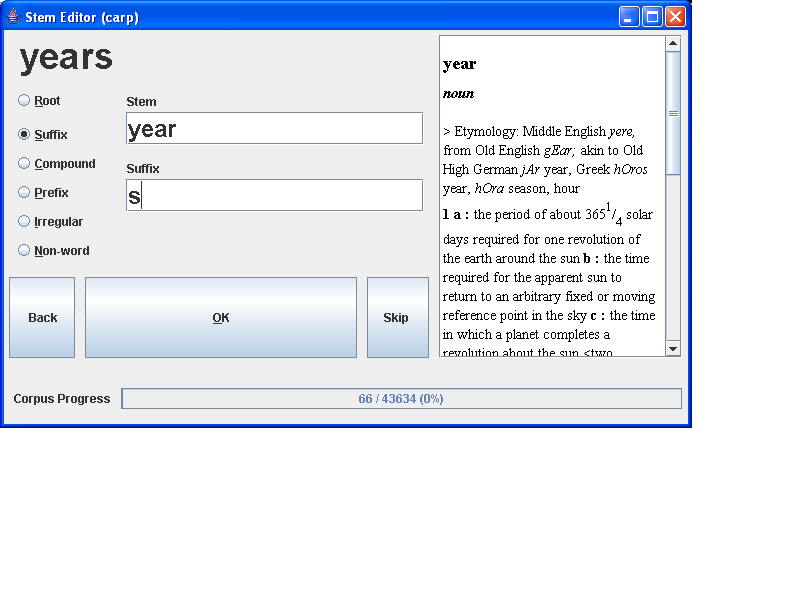
\includegraphics[width=0.95\textwidth]{editor.png}
\caption{Screen shot of editor tool}%
\label{editor-fig}
\end{figure}
%
A screen shot of the tool is provided in figure~\ref{editor-fig}.  It
shows the word to annotate at the top.  Below the word as title is a
list of radio buttons used to select the type of the analysis.  For
instance, in the screen shot, the analysis ``suffix'' is selected,
indicating the word is composed of a stem plus a suffix.  Based on the
word type, fields to the right are available for entering the
components.  For the word {\tt years}, that's a stem {\tt year} and
suffix {\tt s}.  Note that the stem and suffix do not need to form the
word by pure concatenation; for radical cases (e.g. {\tt are} stemming
to {\tt be} or {\tt shake} stemming to {\tt shook}, there is an
``irregular'' analysis type).  Annotators may also mark a word
as a non-word to correct errors in corpus extraction.

To help with the annotation, the application downloads the dictionary
definition from {\tt dictionary.com} over the web and displays it in
HTML.  This is often useful for exploring the etymology of words whose
morphological structure is unclear.

The analyzer is designed to perform a single analysis of a word at a
time.  Thus a word like {\tt ridiculously} would be analyzed as stem
{\tt ridiculous} and suffix {\tt -ly}, rather than a triple of {\tt
ridicule} + {\tt -ous} + {\tt ly}.  To make sure full analyses are
carried out for every word, all stems generated in the tool must be
added to the set of words to analyze.

Once the analysis of a word is complete, the annotator clicks the
``OK'' button, which is nice and fat in compliance with Fitts' law
(time to move the mouse to an area is inversely proportional to target
size).  Annotators may skip entries to return to later and there's a
``Back'' button in order to navigate the previous analysis stack; this
is useful because click brainos are not uncommon when annotating at
speed.  At the very bottom is a list of progress on a corpus.

The annotator is instrumented to populate analyses with the automatic
stem+suffix analyses produced by our unsupervised stemmers.  Elements
to annotate are chosen in order of frequency.  With active learning,
these would be chosen by a risk estimate, which we would define by:
\[
\textrm{risk}(\sigma)
= \textrm{count}(\sigma) \cdot (1 - p(\textrm{firstBest}(\sigma) | \sigma))
\]
This is just the expected number of errors arising from analyzing the
word $\sigma$.  Here $\textrm{firstBest}(\sigma)$ is meant to indicate
the first-best analysis of $\sigma$, and the probability term is the
model's probability estimate for the first best analysis given the
input.  Thus one minus this number is the model's estimate of the
chance of error in assigning the first-best analysis to $\sigma$.
This is all then scaled by the count of $\sigma$, yielding the
expected number of errors arising from the word.  Note that this count
may be scaled to a probability to make the risk figures comparable
across corpora of different counts.

Every time a word is analyzed as anything other than a root or
non-word, its count is added to the stem count.  Note that compounds
include two stems and thus {\tt basketball} would add its count to
{\tt basket} and {\tt ball}, as getting the full analysis right
depends on getting both subanalyses correct.

Training and decoding the general model is straightforward given
training data (see, e.g., Wicentwoski 2004).



\chapter{Conclusions}

For information retrieval applications, simple affix-stripping and
decompounding algorithms work as well, on average, as more
sophisticated morphologically sound approaches.  Without further
detailed evaluations in the context of particular languages and
particular applications, it's unclear whether the more sophisticated
stem-and-suffix sensitive EM methods developed here will actually
improve performance.

Our overall recommendation is to use multiple stems, if possible,
along with the original word in a TF/IDF setting.  This kind of
indexing is supported by Apache Lucene's {\tt TokenStream} interface
to indicate that full forms and their stem occupy the same token
position.  In this way, the high recall of a stemming approach is
preserved, while also preserving most of the precision benefits of
full-form indexing.  These benefits hold not only for single-word
queries, but also for phrasal queries.  The only drawback is index
size and query retrieval speed.

For developing high quality morphological analyses of languages,
including highly sensitive stemmers, we believe labeled training data
is necessary.  Given the low cost of annotating 20,000 examples (one
person week), it seems an obvious win for accuracy under any approach.
From Wicentowski's (2004) word frame model, it appears this may result
in a very high accuracy stemmer (in the mid 90\% accuracy range across
a variety of alnguages).

In terms of supervision, the ``unsupervised'' methods work without
labeled training data, but require a more subtle form of input: tuning
by a statistical computational linguist sensitive to the facts of the
language at hand.  Because we didn't know any of the target languages
other than English, the actual performance figures for our work in
non-English languages is subject to finding evaluation data and tuning
the various EM parameters.



\chapter*{References}
\addcontentsline{toc}{chapter}{References}

\noindent
Adamson, G.\ and J.~Boreham. 1974.
The use of an association measure based on character structure to
identify semantically related pairs of words and document titles.
{\it Information Storage and Retrieval} {\bf 10}.
\\[6pt]
Ando, R.~K.\ and Lillian Lee. 2000.
Mostly unsupervised statistical segmentation of Japanese: application to Kanji.
{\it NAACL 2000}.
\\[6pt]
Antworth, Evan L. 1990.  PC-KIMMO: a two-level processor for
morphological analysis. {\it Occasional Publications in Academic Computing}
{\bf 16}. Summer Institute of Linguistics, Dallas.
\\[6pt]
Argamon, Shlomo, Navot Akiva, Amihood Amir and Oren Kapah.
2004.
Efficient unsupervised recursive word segmentation using
minimum description length.  {\it Proceedings of COLING}.
\\[6pt]
Baroni, Marco, Johannes Matiasek, and Harald Trost.
2002.
Unsupervised discovery of morphologically related words based on orthographic and
semantic similarity.
{\it ACL SIGPHON Workshop}.
\\[6pt]
Bauer, L. 1983.
{\it English Word Formation}.
Cambridge University Press.
\\[6pt]
Baayen, R, R. Piepenbrock, and L. Gulikers. 1995.
The CELEX lexical database.  Release 2.  CD-ROM.
\\[6pt]
Bernhard, Delphine. 2005.
Unsupervised morphological segmentation based on segment
predictability and word segments alignment.
In {\it Proceedings of MorphoChallenge 2005}.
\\[6pt]
Bordag, Stefan. 2005a.
Unsupervised knwoledge-free morpehme boundary detection.
{\it Proceedings of RANLP 05}.
\\[6pt]
Bordag, Stefan. 2005b.
Two-step approach to unsupervised morpheme segmentation.
{\it Proceedings of MorphoChallenge 2005}.
\\[6pt]
Brent, Michael. 1999.
An efficient, probabilistically sound algorithm for segmentation and word discovery. {\it Machine Learning} {\bf 34}:71--106.
\\[6pt]
Buckwalter, Tim. 2004.  Issues in Arabic orthography and morphology
analysis.  {\it Proceedings of the Workshop on Computational
Approaches to Arabic Script-based Languages, COLING 2004}.
\\[6pt]
Carpenter, Bob.  2004.  Scaling language models to gigabytes.
In {\it Proceedings of the ACL Software Workshop}.
\\[6pt]
Chan, Erwin. 2006.
Learning probabilistic paradigms for morphology in a latent class model.
{\it ACL SIGPHON Workshop}.  69--78. Brooklyn.
\\[6pt]
Chomsky, Noam and Morris Halle. 1968.
{\it The Sound Patterns of English}.
Harper and Row.
\\[6pt]
Church, Kenneth and Patrick Hanks. 1990.
Word association norms, mutual information, and lexicography.
{\it Proceedings of ACL 27}, 76--83.
\\[6pt]
Church, Kenneth Ward.  1995.  One term or two?
{\it ACM SIGIR 18}:310-318.
\\[6pt]
Cretuz, Mathias and Krista Lagus. 2002.
Unsupervised discovery of morphemes.
{\it ACL SIGPHON Workshop}, 21--30.
\\[6pt]
Cretuz, Mathias and Krista Lagus. 2005.
Inducing the morphological lexicon of a natural language from unannotated text.
In {\it Proceedings of the International and Interdisciplinary Conference on
Adaptive Knowledge Representationa nd Reasoning}, 106--113.
\\[6pt]
Dalrymple, M., R.~Kaplan, L.~Karttunen, K.~Koskenniemi, S.~Shaio, and M.~Westcoat.
1987.  Tools for morphological analysis.
{\it CSLI Technical Report} CL-87-108. Stanford University.
\\[6pt]
Dawson, J. 1974.
Suffix removal and word conflation.
{\it ALLC Bulletin}.
\\[6pt]
D\'ejean, Herv\'e. 1998.
Morphemes as necessary concepts for structure discovery
from untagged corpora.  In {\it NeMLaP3/CoNLL98 Workshop on Paradigms and
Grounding in Natural Language Learning}, 295--299.
\\[6pt]
Deligne, Sabine and Fr\'ed\'eric Bimbot. 1997.
Inference of varaible-length linguistic and acoutstic units by multigrams.
{\it Speech Communication} {\bf 23}:223--241.
\\[6pt]
Dempster, A.~P., N.~M.~Laird, D.~B.~Rubin. 1977. Maximum likelihood
from incomplete data via the EM algorithm.  {\it Journal of the Royal
Statistical Society}, Series B {\bf 39}:1--38.
\\[6pt]
Dhillon, I.~S., S.~Mallela, and D.~S.~Modha. 2003.
Information-theoretic co-clustering. Technical Report
TR-03-12, Dept. of Computer Science, U. Texas at
Austin.
\\[6pt]
Dzeroski, S.\ and T.~Erjavec. 1997.
Induction of Slovene nominal paradigms.
In {\it Porceedings of the 7th International Workshop
on Inductive Logic Programming}.
\\[6pt]
Namer, Fiammetta and Pierre Zweigenbaum. 2004.  Acquiring meaning for
French medical terminology: contribution of morphosemantics.  In {\it
Proceedings of Medinfo. 2004} {\bf 11}:535--539.
\\[6pt]
Freitag, Dayne.  2005.
Morphology induction from term clusters.
{\it Proceedings of CoNLL}.
\\[6pt]
Gaussier, \'Eric. 1999. Unsupervised learning of derivational
morphology from inflectional lexicons.  {\it ACL 1999 Workshop:
Unsupervised Learning in NLP}.
\\[6pt]
Gelman, Andrew, John B.~Carlin, Hal S.~Stern and Donald B.~Rubin.
2003.
{\it Bayesian Data Analysis (2nd Edition)}.
Chapman and Hall.
\\[6pt]
Goldsmith, John. 2001. Unsupervised learning of the morphology of a
natural language. {\it Computational Linguistics} {\bf
27}(2):153--198.
\\[6pt]
Goldwater, Sharon and Mark Johnson. 2005.  Representational bias in
unsupervised learning of syllable structure.  {\it 9th Conference on
Natural Language Learning}:112--119. Ann Arbor.
\\[6pt]
Graff, David.  2003.  {\it English Gigaword}.
Catalog No.~LDC2003T05.  Linguistic Data Consortium, Philadelphia.
\\[6pt]
Hammarstr\"om, Harald.  2006.  A naive theory of affixation and an algorithm for extraction.  {\it SIGPHON Workshop at NAACL 2006}.
\\[6pt]
Hafer, Margaret A.\ and Stephen F.~Weiss. 1974.
Word segmentation by letter successor varieties.
{\it Information Storage and Retrieval} {\bf 10}:371--385.
\\[6pt]
Hakkani-T\"ur, D.~Z., G.~Oflazer and G.~T\"ur. 2000.  Statistical
morphological disambiguation for agglutinative languages.  {\it
Proceedings of COLING}.
\\[6pt]
Harman, Donna. 1991. How effective is suffixing?
{\it Journal of the American Society for Information Science}
{\bf 42}(1):7--15.
\\[6pt]
Harris, Zellig. 1955.  From phoneme to morpheme.  {\it Language} {\bf
31}:190-222.
\\[6pt]
Harris, Zellig. 1967. Morpheme boundaries within words: report on a
computer test.  {\it Transformation and Discourse analysis Papers 73},
University of Pennsylvania.
\\[6pt]
Hoeksema, Jacob. 1985.
{\it Categorial Morphology}.
New York, Garland.
\\[6pt]
Hu, Yu, Irina Matveeva, John Goldsmith and Colin Sprague. 2005a.
Refining the SED heuristic for morpheme discovery: a look at Swahili.
{\it ACL Psycho- and Computational-Linguistics Workshop}.
\\[6pt]
Hu, Yu, Irina Matveeva, John Goldsmith and Colin Sprague.  2005b.
Using morphology and syntax together in unsupervised learning.
{\it ACL Workshop on Psycho-Computational Linguistics}.
\\[6pt]
Hull, D.~A. 1996.
Stemming algorithms: a case study for detailed evaluation.
{\it Journal of the American Society for Information Science}
{\bf 47}(1): 70--84.
\\[6pt]
Karagol-Ayan, Burcu, David Doermann, and Amy Weinberg. 2006.
Morphology induction from limited noisy data using approximate
string matching.
{\it ACL SIGPHON Workshop}.  60--68. Brooklyn.
\\[6pt]
Jacquemin, Christian. 1997.
Guessing morphology from terms and corpora.
In {\it Proceedings of the ACM SIGIR Conference}.  156--165.
\\[6pt]
Jain, Anil K.\ and Richard Dubes. 1988.
{\it Algorithms for Clustering Data}.  Prentice-Hall.
\\[6pt]
Jain, Anil K., M.~Narasimha Murty and P.~J.\ Flynn. 1999.  Data
clustering: a review. {\it ACM Computing Surveys} {\bf
31}(3):264--323.
\\[6pt]
Jansche, Martin. 2003.  Parametric models of linguistic count data.
{\it 41st Meeting of the Association for Computational Linguistics}.
\\[6pt]
Johnson, C.~Douglas. 1972.
{\it Formal Aspects of Phonological Description}.
Mouton.
\\[6pt]
Johnson, Howard and Joel Martin. 2003.
Unsupervised learning of morphology for English and Inuktitut.
{\it ACL-HLT}.
\\[6pt]
Jordan, Chris, John Healy and Vlado Keselj. 2005.
Swordfish: using ngrams in an unsupervised approach to morphological
analysis.  In Kurimo, Mikko, ed., {\it MorphoChallenge 2005}.
\\[6pt]
Karttunen, Lauri. 1983.
KIMMO: A general morphological processor.
{\it Texas Linguistic Forum} {\bf 22}: 165--186.
\\[6pt]
Karttunen, L., K.~Ga\'al, and A.~Kempe.  1997.
{\it Xerox Finite-State Tool}.
Xerox Research Center, Grenoble.
\\[6pt]
Karttunen, Lauri and Kenneth R.~Beesley. 2001.
History of two-level morphology.
{\it ESSLLI 2001}.
\\[6pt]
Kazakov, D. 1997.
Unsupervised learning of naive morphology with genetic algorithms.
{\it ECML/Mlnet Workshop on Empirical Learning of NLP Tasks}.
\\[6pt]
Kazakov, Dimitar and Suresh Manadhar. 2001.
Unsupervised learning of word segmentation rules with genetic
algorithms and inductive logic programming. {\it Machine Learning} {\bf 43}:121--162.
\\[6pt]
Kit, Chunyu and Yorkick Wilks.  1999. Unsupervised learning of word
boundary with description length gain.  {\it Conference on Natural
Language Learning}.
\\[6pt]
Kleinberg, J.~M. 1998. Authoritative sources in a hyperlinked
environment.  In {\it Proceedings of the ACM-SIAM Symposium on
Discrete Algorithms}.
\\[6pt]
Koskenniemi, Kimmo. 1983.  {\it Two-Level Morphology: A General
Computational Model for Word-Form Recognition and Production}.
Ph.D.\ thesis, University of Helsinki.
\\[6pt]
Krovetz, Robert. 1993. Viewing morphology as an inference process.
{\it SIGIR 16}:191--202.
\\[6pt]
Kurimo, Mikko, Mathias Creutz, Matti Varjokallio, Ebru Arisoy and
Murat Saraclar.  . 2005.  Unsupervised segmentation of words into
morphemes -- Challenge 2005:an introduction and evaluation report.  In
{\it EU Pascal Challenge: Unsupervised segmentation of words into
morphemes}.
\\[6pt]
Lari, K. and S. Young. 1990. The estimation of stochastic context-free grammars using the Inside-Outside algorithm. Computer Speech and Language, {\bf 4}:35-56.
\\[6pt]
Lennon, M., D.~S.~Pierce, B.~D.~Tarry, P.~Willet. 1981.
An evaluation of some conflation algorithms for information retrieval.
{\it Journal of Information Science} {\bf 3}:177--183.
\\[6pt]
Ling, C.~X. 1994.  Learning the past tense of English verbs: the
symbolic pattern associator vs.\ connectionist models.  {\it Journal
of Artificial Intelligence Research} {\bf 1}:209--229.
\\[6pt]
Lovins, J.~B. 1968.
Development of a stemming algorithm.
{\it Mechanical Translation and Computational Linguistics}
{\bf 11}.
\\[6pt]
Lovins, J.~B. 1971. Error evaluation for stemming algorithms as clustering algorithms. {\it Journal of the American Society for Information Sciences}{\bf 22}:28-40.
\\[6pt]
Luk, Robert W.~P., K.~F.~Wong, K.~L.~Kwok.
2002.
Hybrid term indexing: an evaluation.
{\it Proceedings of the 3rd NTCIR Workshop}
\\[6pt]
MacKay, David J.~C., Linda C.~Bauman Peto. 1994.
A hierarchical Dirichlet language model.
{\it Natural Language Engineering} {\bf 1}(3):1--19.
\\[6pt]
MacWhinney, B. 1978.
{\it The Acquisition of Morphophonology}.
Monographs of the Society for Research in Child Development {\bf 43}.
\\[6pt]
Manning, Christopher D. 1998.
The segmentation problem in morphology learning.
In {\it NeMLaP3/CoNLL98 Workshop on Paradigms and Grounding
in Language Learning}, 299--305.
\\[6pt]
Marchand, H. 1969.
{\it The Categories and Types of Present-Day English Word Formation}.
C.~H. Beck.
\\[6pt]
Martin, W., B.~Al, and P.~Sterkenburg. 1983.  On the processing of a
text corpus: from textual data to lexicographical information.In
R.~Hartman (ed.), {\it Lexicography, Principles and Pracitce}, 77--87.
Academic Press.
\\[6pt]
Mastroianni, Michael and Bob Carpenter. 1994. Constraint-based
Morpho-phonology. In Proceedings of the First ACL SIGPhon
Workshop. Las Cruces, New Mexico.
\\[6pt]
Maxwell, Mike. 2002.
Resources for morphology learning and evaluation.
{\it LREC}.
\\[6pt]
McNamee, Paul. 2003. Knowledge-light Asian language text retrieval at the NTCIR-3 workshop.
{\it Proceedings of the 3rd NTCIR Workshop}.
\\[6pt]
McCray, A., A.~Browne, and D.~Moore.  1988.
The semantic structure of neo-classical compounds.
In {\it SCAMC'88 -- Proceedings of the 12th Annual Symposium on
Computer Applications in Medical Care}, 165--168.
\\[6pt]
Mikheev, A.. 1997. Automatic rule induction for
unknown-word guessing. {\it Computational Linguistics}
{\bf 23}(3):405--423.
\\[6pt]
Monson, Christian.  2004.  A framework for unsupervised natural language morphology induction.  {\it 2004 ACL Student Workshop}.
\\[6pt]
Monson, Christian, Alon Lavie, Jaime Carbonell and Lori Levin. 2004.
Unsupervised induction of natural language morphology inflection classes.
{\it ACL SIGPHON}.
\\[6pt]
Neuvel, Sylvain and Sean A.~Fulop. 2002.
Unsupervised learning of morphology without morphemes.
In {\it ACL SIGPHON Workshop}, 31--40.
\\[6pt]
Nevill-Manning, Craig G.\ and Ian H.\ Witten. 1997.  Identifying
hierarchical structure in sequences: a linear time algorithm.  {\it
Journal of Artificial Intelligence Research} {\bf 7}:67--82.
\\[6pt]
Nie, Jian-Yun, Jiangfeng Gao, Jian Zhang and Ming Zhou.
2000.
On the use of words and n-grams for Chinese information retrieval.
{\it Proceedings for the 5th International Workshop on Information
Retrieval with Asian Languages}.
\\[6pt]
Oflazer, K., S.~Nirenberg and M.~McShane. 2001.  Bootstrapping
morphological analyzers by combining human elicitation and machine
learning.  {\it Computational Linguistics} {\bf 27}(1):59--84.
\\[6pt]
Paice, C.~D. 1996.
Method for evaluation of stemming algorithms based on error counting.
{\it Journa l of the American Society for Information Science}
{\bf 47}(8):632--649.
\\[6pt]
Peng, Fuchun and Dale Schuurmans. 2001.
A hierarchical EM approach to word segmentation.
{\it 6th NLP Pacific Rim Symposium}.
\\[6pt]
Pereira, Fernando and Yves Schabes. 1992.
Inside-outside reestimation from partially bracketed corpora.
In {\it ACL}.
\\[6pt]
Porter, Martin. 1980. An algorithm for suffix stripping. {\it Program}
{\bf 14}(3):130--137.
\\[6pt]
Quasthoff, U.; M. Richter; C. Biemann. 2006. Corpus Portal for Search
in Monolingual Corpora, In {\it Proceedings of the Fifth International
Conference on Language Resources and Evaluation}, LREC 2006, Genoa.
\\[6pt]
Quasthoff, Uwe and Christian Wolff. 2002.
The Poisson collocation measure and its applications.
In {\it Proceedings of the Second International Workshop
on Computational Approaches to Collocations}.
\\[6pt]
Rayson, Paul and Roger Garside. 2000.
Comparing corpora using frequency profiling.
In {\it Proceedings of the ACL Workshop on Comparing Corpus}, 1--6.
\\[6pt]
Reape, Michael. 1989.  A Logical Theory of Semi-Free Word Order and
Bounded Discontinuous Constituency. In {\it Proceedings of the
EACL}. Manchester, England.
\\[6pt]
Redlich, A.~Norman. 1993.
Redundancy reduction as a strategy for unsupervised learning.
{\it Neural Computation} {\bf 5}:289--304.
\\[6pt]
Rissanen, Jorma.  1983. A universal prior for integers and estimation
by minimum description length. {\it Annals of Statistics} {\bf
11}(2):416--431.
\\[6pt]
Rissanen, Jorma. 1989.
{\it Stocastic Complexity in Statistical Inquiry}.
World Scientific Publishing.
\\[6pt]
Rumelhart, D.~E.\ and J.~L.~McClelland. 1986.
On learning the past tenses of English verbs.
In J.~L.~McClelland and D.~E.~Rumelhart (eds.),
{\it Parallel Distributed Processing: Explorations
in the Microstructure of Cognition}, Volume 2, 216--271.
MIT Press.
\\[6pt]
Saffran, Jenny R., Elissa L.~Newport, and Richard N.~Aslin.
1996.
Word segmentation: the role of distributional cues.
{\it Journal of Memory and Language} {\bf 35}(4):606--621.
\\[6pt]
Salton, Gerald and M.~Lesk. 1968.
Computer evaluation of indexing and text processing.
{\it Journal of the ACM} {\bf 15}(1):8--36.
\\[6pt]
Schone, Patrick and Daniel Jurafsky. 2001. Knowledge-free induction of
inflectional morphologies. {\it NAACL 2001}.
\\[6pt]
Schulz, Stefan, Martin Honeck and Udo Hahn. 2002.
Biomedical text retrieval in languages with
a complex morphology.  In {\it Proceedings of the ACL
Workshop on NLP in the Biomedical Domain}, 61--68.
\\[6pt]
Sch\"utzenberger, M.~P. 1961.
A remark on finite transducers.
{\it Information and Control} {\bf 4}:185-196.
\\[6pt]
Snover, Matthew G.\ and Michael R.~Brent.
2002.
A probabilistic model for learning concatenative morphology.
{\it NIPS 2002}.
\\[6pt]
Sproat, Richard.  1992.
{\it Morphology and Computation}. MIT Press.
\\[6pt]
Su, K.\ M.~Wul and J.~Chang. 1994.
A corpus-based approach to automatic compound extraction.
{\it 32nd ACL}.  Las Cruces, NM.
\\[6pt]
Swanson, Don. 19??.
\\[6pt]
Theron, P.\ and I.~Cloete. 1997.
Autmatic acquisition of two-level morphological rules.
{\it Proceedings of the Fifth ANLP}, 103--110.
\\[6pt]
Wicentowski, Richard. 2004. Multilingual noise-robust supervised morphological analysis using the WordFrame model. {\it ACL SIGPHON 2004}. Barcelona.
\\[6pt]
Xanthos, Aris, Yu Hu, and John Goldsmith. 2006.
Exploring variant definitions of pointer length in MDL.
{\it ACL SIGPHON Workshop}.  32--40. Brooklyn.
\\[6pt]
Xu, Jinxi and W.~Bruce Croft. 1998. Corpus-based stemming using cooccurrence of word variants.  {\it ACM Transactions on Information Systems} {\bf 16}(1):
\\[6pt]
Yarowsky, David and Richard Wicentowski. 2000.
Minimally supervised morphological analysis by multimodal alignment.
{\it Proceedings of ACL}, 207--216.
\\[6pt]
Yarowsky, David, Grade Ngai, and Richard Wicentowski. 2001.
Inducing multilingual text analysis tools via robust
projection across aligned corpora.  {\it Proceedings of HLT}, 161--168.
\\[6pt]
Yu, Hua. 2000. Unsupervised word induction using MDL criterion. {\it
ICSLP}. Beijing.
\\[6pt]
Zipf, George Kingsley. 1968.
{\it The Psychobiology of Language. An Introduction to Dynamic Philology}.
Second Edition. (First edition, 1935)
M.~I.~T.~Press/Cambidge.
\\[6pt]
Zipf, George Kingsley. 1949.
{\it Human Behavior and the Principle of Least Effort}.  Addison-Wesley.
\\[6pt]
Zweigenbaum, Pierre and Natalia Grabar.  1999.  Contribution of
medical terminology to medical language processing: experiments in
morphological knowledge acquisition from thesauri.  In {\it
Proceedings of IMIA Workshop on Natural Language Processing and
Medical Concept Representation}.
\end{document}